\documentclass[11pt,twoside]{book}

% Packages + Config (indented to be folded in vim)
  \usepackage[utf8]{inputenc}
  \usepackage{graphicx}  % to use imgaes, and store them in a shared folder
  \usepackage{times}
  \graphicspath{{images/}}
  \usepackage{caption}   % to have caption on different parts of a figure
  \usepackage{subcaption}
  \usepackage{booktabs}  % better looking tables
  \usepackage{multirow}
  \usepackage{hyperref}  % to have clickable links when a paper is cited
  \usepackage{bookmark}  % so conclusion is not in last part (part III)
  \usepackage{natbib}    % to cite paper and set a nice style for bibliography
  \usepackage{fancyhdr}  % to print the name of section in header/footer
  \usepackage{xcolor}    % to write some words in color
  \usepackage{amsmath}   % for multiline equations
  \usepackage{amsfonts}  % for some symbols in \equation
  \usepackage{amsthm}    % to write theorems and definitions
  \usepackage{pgfplots}  % for plots build from inside the .tex file
  \usepackage[a4paper,   % default margins of a book are large, reduce them
              width=150mm,top=25mm,bottom=25mm,bindingoffset=6mm]{geometry}

  % I HATE TO TYPE \textcolor{red}{bla...bla} each time I want something red
  \newcommand{\red}[1]{(\textcolor{red}{#1})}

  % Keyboard shortcut for bold teal things for subscript text and normal text
  % (used in tables of ch05 - dict2vec)
  \newcommand{\indic}[1]{$_{\textcolor{teal}{\textbf{#1}}}$}
  \newcommand{\teal}[1]{\textcolor{teal}{\textbf{#1}}}

  % \autoref by default does not capitalize chapter/section/subsection. Make
  % them Titlecase (first letter in uppercse)
  \def\chapterautorefname{Chapter}
  \def\sectionautorefname{Section}
  \def\subsectionautorefname{Subsection}

  % Configure the information displayed in header/footer of each page
  % *** MODIFIED AGAIN IN chapter/01-...tex ***
  \pagestyle{fancy}  % L=left, R=right, C=center, O=odd pages, E=even pages
  \renewcommand{\chaptermark}[1]{ \markboth{#1}{} }
  \renewcommand{\sectionmark}[1]{ \markright{#1}{} }
  \fancyhf{} % set header/footer empty (to override the default info)
  % Even pages: pageNumberInBold chapterTitle             chapterNumber
  % Odd pages:  sectionNumber             sectionTitle pageNumberInBold
  \fancyhead[LE]{\textbf{\thepage}~~~\textit{\leftmark}}
  \fancyhead[RE]{\MakeUppercase{\chaptername}~\thechapter}
  \fancyhead[LO]{\textit{\rightmark}}
  \fancyhead[RO]{\textbf{\thepage}}
  \renewcommand{\headrulewidth}{0pt} % width of horizontal rule below header

  % Define some custom colors, used in one example in ch05 - dict2vec
  \definecolor{maroon}{rgb}{215,0,0}
  \definecolor{cobalt}{rgb}{0.0, 0.28, 0.67}
  \definecolor{cerise}{rgb}{0.87, 0.19, 0.39}
  \definecolor{jade}{rgb}{0.0, 0.66, 0.42}

  % Special argmin/argmax with things underneath (used in optimization equation)
  \DeclareMathOperator*{\argmin}{arg\,min}
  \DeclareMathOperator*{\argmax}{arg\,max}

  % To have some definitions or theorems or lemma
  \newtheorem{theorem}{Theorem}[chapter]
  \theoremstyle{definition}
  \newtheorem{definition}{Definition}[chapter]
  \newtheorem{lemma}{Lemma}[chapter]

  % How to cite papers:
  %   \citet{}       Textual citation
  %   \citep{}       Parenthetical citation
  %   \citet*{}      Same as \citet but if there are several authors, all
  %                  names are printed
  %   \citep*{}      The same as \citep but if there are several authors, all
  %                  names are printed
  %   \citeauthor{}  Prints only the name of the authors(s)
  %   \citeyear{}    Prints only the year of the publication.

% Main parts of the thesis
\begin{document}

  % Page de garde -> avant tout le reste
    \newgeometry{centering} % pour que la page de garde soit centree
    \begin{titlepage}
\begin{center}
  % 0.72 to have the same ratio as in the .doc given by the university
  
\includegraphics[width=0.72\linewidth]{ch000-logo-university}

  \vspace{3em}
  {\Large \textbf{THESE DE DOCTORAT DE L’UNIVERSITE DE LYON}}

  \vspace{0.6em}
  opérée au sein de\par
  l'\textbf{Université de Saint-Etienne}\par
  \vspace{0.1em}
  {\small N$^\circ$ d’ordre NNT : 2020LYSES008}

  \vspace{1.6em}
  Ecole Doctorale \textbf{ED SIS 488} \par
  \textbf{Science, Ingénierie et Santé}

  \vspace{1.6em}
  Spécialité de doctorat : \textbf{Informatique}

  \vspace{1.6em}
  {\large Thèse préparée par \textbf{Julien Tissier} \par}
  \vspace{0.1em}
  {\large Soutenue le 4 mai 2020}

  \vspace{1em}

  \rule{\textwidth}{1pt}

  \vspace{0.8em}
  {\Large \textbf{Improving methods to learn word representations\\}}
  \vspace{0.6em}
  {\Large \textbf{for efficient semantic similarities computations}}
  \vspace{0.8em}

  \rule{\textwidth}{1pt}

  \vspace{2em}
  Devant le jury composé de :

  \begin{table}[h]
    \resizebox{\textwidth}{!}{
    \centering
    \begin{tabular}{@{}llll@{}}
      \toprule[0.12em]
      Massih-Reza AMINI  & Professeur            &
      Université Grenobles Alpes                 & Rapporteur\\

      Julien VELCIN      & Professeur            &
      Université de Lyon 2                       & Rapporteur\\

      Elisa FROMONT      & Professeure           &
      Université de Rennes 1                     & Examinatrice\\

      Laure SOULIER      & Maître de Conférences &
      Sorbonne Université                        & Examinatrice\\

      Christophe GRAVIER & Maître de Conférences &
      Université de Saint-Etienne                & Directeur de thèse\\

      Amaury HABRARD     & Professeur            &
      Université de Saint-Etienne                & Co-directeur de thèse\\
      \bottomrule[0.12em]
    \end{tabular}}
  \end{table}

\end{center}
\end{titlepage}

    \thispagestyle{empty} % no header in the page after cover page = blank page
    \restoregeometry %  pour que les pages suivantes ne soient plus centrees
    % (dans la documentclass book, les marges des pages gauche et droite ne sont
    % pas les meme, elles sont inversees, avec une plus grande marge sur le cote
    % exterieur de la page).

  % Table of Contents (written as "Contents")
    % Evite que le header dans le TOC ait "CHAPTER 0" ou "CONTENTS" (qui est le
    % default behavior)
    \fancyhead[LE]{\textbf{\thepage}}
    \fancyhead[RE]{\textit{Contents}}
    \fancyhead[LO]{\textit{Contents}}
    \fancyhead[RO]{\textbf{\thepage}}
    \setcounter{tocdepth}{1} % does not add subsection into table of contents
    \tableofcontents

  % Introduction
    % No chapter number for Intro, so need to place it manually in Table of
    % Content with \addcontentsline
    \chapter*{Introduction}
    \addcontentsline{toc}{chapter}{Introduction}
    \fancyhead[LE]{\textbf{\thepage}}
\fancyhead[RE]{\textit{Introduction}}
\fancyhead[LO]{\textit{Introduction}}
\fancyhead[RO]{\textbf{\thepage}}

Natural Language Processing (NLP) is a branch of Artificial Intelligence that
aims to make machines able to process and understand information from the human
language in order to solve some specific tasks, like translating a document or
automatically writing reports from market data. In the context of this thesis,
we focus on textual information, which can be found in webpages, books,
communication applications, etc. With the democratization of the Internet, the
amount of written and shared textual information has never been so important.
For example, each second\footnote{As of March 2020, according to
\url{https://www.internetlivestats.com/one-second/} .}, almost 9,000
tweets\footnote{A \textit{tweet} is a short message (up to 280 characters)
posted on the website \url{https://www.twitter.com} .} are published and almost
3 million emails are sent. Being able to process this large amount of data to
extract meaningful information can no longer be achieved manually, and for this
reason, the development of NLP models have rapidly gained interest within the
last couple of years to do it automatically. These models have become more and
more complex in order to solve more and more difficult tasks, like with
self-generating dialog systems (chatbots) or with personal assistants (Siri,
Alexa, etc.). Unlike humans, these models do not directly process words to solve
a given task. Most of the NLP models are based on Machine Learning (a
subfield of Artificial Intelligence) models which commonly use vectors as a
representation of data in order to apply some algorithms and solve the task.
Therefore, before solving a task, a common preliminary step of NLP models is to
represent the elements one can find in textual information as vector
representations. \medskip

In this thesis, we are interested in methods used to generate those vector
representations of textual information, and more specifically, representations
of words since they are the most basic unit one can find in a text. These word
representations are called \textit{word embeddings} and are typically
represented as an array of values. Word embeddings are then used in downstream
NLP models to solve tasks. The values in word embeddings have to be set such
that they reflect the linguistic properties of words and the relations between
them. Indeed, they are the main source of information the downstream models have
access to in order to solve the task. Without linguistic information encoded
into word embeddings, the models would not have any knowledge to know how to use
the word vectors and give the expected answer or the correct prediction for a
given task. The first works on word embeddings manually created word vectors by
using specific linguistic properties of words, generated by linguistic experts.
However, these methods are not scalable when the number of words to embed is in
the order of millions, which is commonly the case for popular languages like
English and the massive amount of textual data available on the Web. Therefore,
to overcome this shortcoming, some methods have been developed to automatically
learn word embeddings. They are usually based on the statistics of the
occurrences of words in texts to learn word representations that convey
linguistic information. These methods are mostly \textit{unsupervised}: there
are no clues or hints given to the method to know which linguistic information
should be encoded into the embeddings, or which word vectors should be related.
\bigbreak

During the last decade, many different methods have been created to learn word
embeddings that capture linguistic information in order to be used in downstream
NLP models to solve tasks. Among these methods, two main limitations can be
observed:

\begin{itemize}
  \item Most of the methods learn word embeddings with statistics from large
    training texts extracted from the Web. These texts are, for the majority,
    generic and do not contain many specific linguistic information, which is
    therefore not captured into the word embeddings learned by these methods.
  \item As the tasks to solve become more difficult, the linguistic knowledge
    required to solve them increases, and so is the complexity and the size of
    the methods that learn to encode this additional knowledge into word
    embeddings. With the democratization of NLP applications running on
    low-resource devices like smartphones, such complex and large word
    representations models cannot be used on those devices.
\end{itemize}

\noindent These two limitations of current word embeddings are complementary: if
more linguistic information is encoded into word vectors with other sources of
information, the representations would become larger and would not be able to
run on low-resource devices. On the other hand, if the word vectors are reduced
by removing some of their values to be able to run on low-resource devices, the
amount of information they encode would also be reduced. The contributions
presented in this thesis address each one of these limitations.

\subsubsection{Contributions}
  This thesis presents two contributions to learn word embeddings which address
  the two aforementionned limitations of current word embeddings. The first
  contribution is a novel method that uses lexical dictionaries to extract
  semantic relations between words and incorporate this additional information
  in a model to learn word embeddings. The process of extracting information
  from dictionaries is based on the cooccurrence of words in their dictionary
  definitions and is completely automatic. The word embeddings learned with this
  method exhibit significant improvements in word semantic similarity tasks
  compared to other common word embeddings learning methods. This first
  contribution has been accepted and presented at the EMNLP 2017 conference
  \citep{tissier2017dict2vec}. The second contribution is a method to transform
  common word embeddings (which usually use real values to encode information)
  into binary word vectors. The binary vectors are much smaller in memory than
  the real-valued ones (more than 30 times smaller) and have the advantage of
  accelerating vector operations, which are two of the main characteristics
  required to be used in downstream models on low-resource devices. This second
  contribution has been accepted and presented at the AAAI 2019 conference
  \citep{tissier2019near}.

\subsubsection{Outline}
  This thesis is divided into three main parts:~\autoref{chap:preliminaries}
  and~\autoref{chap:ml-for-we} introduce the main notions and concepts used
  throughout this thesis;~\autoref{chap:methods-we}
  and~\autoref{chap:methods-reduction} give an overview of the existing methods
  to learn word embeddings and reduce the size of
  representations;~\autoref{chap:dict2vec} and~\autoref{chap:nlb} present the
  two contributions of this thesis. \medskip

    \textbf{Chapter 1} introduces the main notions used in this thesis, the most
    important one being the definition of \textit{word embeddings}. It also
    details tasks to evaluate the quality of word embeddings, which are used in
    the chapters of contributions (\autoref{chap:dict2vec}
    and~\autoref{chap:nlb}). \medskip

    \textbf{Chapter 2} presents the main concepts of machine learning:
    supervised learning, unsupervised learning and semi-supervised learning. It
    also explains how can machine learning models learn from data and presents
    two models (neural network and autoencoder) that are commonly used in the
    word embeddings literature. \medskip

    \textbf{Chapter 3} is an overview of the most common existing methods to
    learn word embeddings. It details different models, from the first works on
    word embeddings to the latest ones which are, as we said before, complex and
    large. Some of the methods presented in this chapter are used
    in~\autoref{chap:dict2vec} to compare the performances of the word
    embeddings learned by the model of the first contribution. \medskip

    \textbf{Chapter 4} is an overview of existing methods to reduce the size of
    vector representations so they can be smaller in memory or speed up vector
    computations. Some of the methods presented in this chapter are used
    in~\autoref{chap:nlb} to compare the performances of the binary word vectors
    learned by the model of the second contribution. \medskip

    \textbf{Chapter 5} presents the first contribution of this thesis. It
    details how additional semantic information is extracted from the dictionary
    definitions of words and how this information is used to learn
    semantically-richer word embeddings. Several tasks like word semantic
    similarity or document classification are used to evaluate the quality of
    those word representations and their performances in downstream models.
    \medskip

    \textbf{Chapter 6} presents the second contribution of this thesis. It
    details the model and its architecture used to transform learned word
    embeddings into binary word vectors of any size. Several evaluations are
    performed to measure the quality of those binary vectors and an additional
    task is performed to evaluate the computational benefits of binary vectors
    for semantic similarity computations.


  % PART 1 = preliminaries + machine learning for WE
    \part{Background}
      \chapter{Preliminaries on Word Representations}
      \label{chap:preliminaries}
      % reset to default value for the next chapters (because intro messed it up)
\fancyhead[LE]{\textbf{\thepage}~~~\textit{\leftmark}}
\fancyhead[RE]{\MakeUppercase{\chaptername}~\thechapter}
\fancyhead[LO]{\textit{\rightmark}}
\fancyhead[RO]{\textbf{\thepage}}

\section{Introduction}
  \label{ch01:sec:introduction}
  A language is a concept allowing one to express some meaning and communicate.
  For this thesis, we will consider languages that can be expressed by means
  of a text. A text can be viewed as a simple entity: a sequence of letters,
  numbers or symbols. But to work with texts and being able to create algorithms
  that can process them, we need to define some terms and notions. Let us define
  what are the main components of a text. The first unit that can be found in a
  text is defined by the notion of \textit{words}.

  \theoremstyle{definition}
  \begin{definition}[A word]
    \label{ch01:def:def-word}
    Let $\Sigma$ be a a finite alphabet representing a non-empty finite set of
    symbols. A word is a finite sequence of symbols from $\Sigma$ that carries a
    meaning.
  \end{definition}

  In this thesis, we are only interested in texts of occidental languages like
  English. Any further mention to \textit{a word} will refer to a sequence of
  letters (from the Roman alphabet), digits or symbols (like punctuation marks
  such as dash ``-'') that carries a meaning. Then, we can assemble words to
  form \textit{sentences}.

  \theoremstyle{definition}
  \begin{definition}[A sentence]
    \label{ch01:def:def-sentence}
    A sentence is a sequence of words, separated by spaces or punctuation
    symbols.  The first word of a sentence starts with an uppercase letter and
    the last word of the sentence is followed by a period (.), a question mark
    (?) or an exclamation mark (!).
  \end{definition}

  Sentences can be then be assembled to form \textit{a text}.

  \theoremstyle{definition}
  \begin{definition}[A text]
    \label{ch01:def:def-text}
    A text is a sequence of sentences.
  \end{definition}

  Another important notion when working with text is the \textit{vocabulary}.

  \theoremstyle{definition}
  \begin{definition}[A vocabulary]
    \label{ch01:def:def-vocabulary}
    The vocabulary of a text is the set of all the unique words which occur in
    this text.
  \end{definition}

  The length of a text should not be confused with the size of its vocabulary.
  Indeed, if a word appears several times in a text, it will be present only
  once in its vocabulary. Therefore, the length of a text is usually way larger
  than the size of its vocabulary. Let us take an example of two short texts to
  illustrate this.~\autoref{ch01:tab:vocabulary-text-example} indicates the
  vocabulary of two short texts.

  \begin{itemize}
    \item Text 1 has a vocabulary size of 17 words but a text length of 23
      words.
    \item Text 2 has a vocabulary size of 17 words but a text length of 20
      words.
  \end{itemize}

  \begin{table}[t]
    \resizebox{\textwidth}{!}{
    \centering
    \begin{tabular}{llcl}
      \toprule[0.15em]
        & Text && Vocabulary\\
      \midrule[0.08em]
      1 & Add the milk to the flour and egg preparation
       && Add, the, milk, to, flour, and, \\

        & and mix it. Do not mix too quickly to avoid
       && egg, preparation, mix, it, Do, not,\\

        & lumps in the preparation.
       && too, quickly, avoid, lumps, in\\
      \midrule

      2 & Liverpool won the final against Tottenham.
       && Liverpool, won, the, final, against, \\

        & Salah scored after 1 minute and Origi scored
       && Tottenham, Salah, scored, after, 1,\\

        & another goal at the 87th minute.
       && minute, and, Origi, another, goal,\\

        &
       && at, 87th\\
      \bottomrule[0.15em]
    \end{tabular}}
    \caption{Examples of short texts and their vocabularies.}
    \label{ch01:tab:vocabulary-text-example}
  \end{table}

  \noindent When we want to talk about the length of a text, we usually use the
  term ``token'' over the term ``word''. For example, we can say that Text 1
  contains 23 tokens (because its text length is 23 words).\medskip

  In the Natural Language Processing (NLP) domain, the final objective is
  usually to solve a given task. This includes for instance text classification
  which consists in finding the correct category of a text. Another task is
  information retrieval which focuses on extracting the correct sentences or
  documents the most relevant to a question. In order to show how the vocabulary
  of a text can be used to solve a given task, let us pick up the example of the
  text classification task. In this task, a naive way to find the correct
  category of a text would be to look at its tokens or at the content of its
  vocabulary and assign the category with the greatest amount of specific words
  (\textit{e.g.} the words ``won'', ``scored'' and ``goal'' of Text 2
  in~\autoref{ch01:tab:vocabulary-text-example} probably indicate that the text
  is about \textit{sport}). However, it is difficult to compare two texts based
  solely on their vocabulary. Some words are different but have the same
  meaning, so two texts can have completely different vocabularies but still
  discuss the same subject or have the same information. The same goes for
  information retrieval, as a sentence can be the perfect answer to a question
  without using any of the words of the question. Therefore, although tokens and
  vocabularies are the essence of texts, there are not sufficient to represent
  the semantic information of the text or to process the content of the
  document. In order to solve this issue, we need additional concepts or
  representations that can be used to work with texts or documents. The next
  section presents some notions that are commonly used in the NLP literature.

\section{From words to numerical representations}
  In the vocabulary of a text, each word only appears once even if it has
  several occurrences in the text. Therefore the vocabulary representation of a
  text is lacking some information, which is a shortcoming to be able to process
  it. If one text contains 20 times the word ``football'' and another text
  contains it only once, there is no way to know which text speaks the most
  about \textit{football} by only looking at their vocabulary because both text
  vocabularies have only a single occurrence of ``football''. One solution to
  this problem is the \textit{Bag-of-Words (BoW)}
  representation~\citep{lang1995newsweeder, joachims1997probabilistic}.

  \theoremstyle{definition}
  \begin{definition}[Bag-of-Words]
    \label{ch01:def:def-bow}
    The Bag-of-Words representation of a text is the set of all the unique words
    within it, and the associated number of occurrence of each word.
  \end{definition}

  \noindent For the two texts of~\autoref{ch01:tab:vocabulary-text-example},
  their Bag-of-Words are:

  \begin{itemize}
    \item Text 1: \\
      \{
      Add:~1,
      the:~3,
      milk:~1,
      to:~2,
      flour:~1,
      and:~2,
      egg:~1,
      preparation:~2,
      mix:~2,
      it:~1,
      Do:~1,
      not:~1,
      too:~1,
      quickly:~1,
      avoid:~1,
      lumps:~1,
      in:~1
      \}
    \item Text 2:\\
      \{
      Liverpool:~1,
      won:~1,
      the:~2,
      final:~1,
      against:~1,
      Tottenham:~1,
      Salah:~1,
      scored:~2,
      after:~1,
      1:~1,
      minute:~2,
      and:~1,
      Origi:~1,
      another:~1,
      goal:~1,
      at:~1,
      87th:~1
      \}
  \end{itemize}

  With Bag-of-Words representations, one can tell if among two texts using the
  same words, one contains more terms related to a subject. But solving this
  problem also introduces another one. In a text, most of the words are
  irrelevant to understand its topic. For example, in Text 2, the words
  ``another'' or ``after'' are less important than ``scored'' or ``goal'' to
  know that the text deals about \textit{football}. Moreover, if a word appears
  in a lot of texts, then it is probably not discriminative to know the topic of
  a text. For instance, the word ``minute'' in Text 2 can also be found in other
  cooking recipes (which is the topic of Text 1) so this word is not indicative
  to differentiate the two different topics. To take into account the fact that
  less important words are usually way more frequent than more specific ones (it
  has been shown empirically that the frequency of words in a text follows a
  Zipf's law) and therefore that the number of occurrences of a word is not an
  indicative information, the values in BoW need to be replaced. The values need
  to measure the importance of a term in a text, but also among a set of texts.
  Words that are frequent among all the texts should have a smaller value
  because they are not discriminative. On the other hand, less frequent words
  should have a higher value because they better characterize a text. One
  solution is to replace the number of occurrences by the \textit{TF-IDF value}.

  \theoremstyle{definition}
  \begin{definition}[TF-IDF]
    The TF-IDF of a word is a statistical value that indicates the importance of
    a word within a text among a collection of texts. It is defined as:
    \begin{equation}
      \text{TF-IDF}(word, text) = tf_{word, text} \times
      \log(\frac{N}{D_{word}})
    \end{equation}
    \label{ch01:def:def-tfidf}
  \end{definition}

  \noindent where $tf_{word, text}$ is the number of occurrences of $word$ in
  $text$, $N$ is the total number of texts and $D_{word}$ is the number of texts
  which contain $word$. With the same texts as
  in~\autoref{ch01:tab:vocabulary-text-example}, we have:

  \begin{itemize}
    \item TF-IDF(``the'', Text 1) = $3 \times \log (\frac{2}{2})$ = 0
    \item TF-IDF(``the'', Text 2) = $2 \times \log (\frac{2}{2})$ = 0
    \item TF-IDF(``milk'', Text 1) = $1 \times \log (\frac{2}{1})$ = 0.693
    \item TF-IDF(``scored'', Text 2) = $2 \times \log (\frac{2}{1})$ = 1.39
  \end{itemize}

  \medskip
  Now that we have introduced the concept of TF-IDF, we can have a
  representation for each document based on the words it contains and the
  importance of each word. This type of representation has been proved to be
  useful for information retrieval~\citep{ramos2003using} or document
  classification~\citep{zhang2011comparative}. However, this representation has
  some severe limitations:

  \begin{enumerate}
    \item In order to compute the similarity of two given texts or to find the
      most specific words in a BoW representation, one has to go through each
      element and compare the words or their value. This becomes a problem when
      the size of the vocabulary is in the order of thousands and the number of
      texts reach several millions.
    \item These representations can be viewed as \textit{manually} generated.
      While the process of finding the unique words and counting their number of
      occurrences can be automated, the definition used to compute the weights
      (\textit{i.e.} the values) in the BoW representations are defined by a
      human, which implies the need of an expert who knows what values would be
      useful for processing texts.
    \item The BoW representation has zero understanding of the semantic and
      syntactic properties of words. Indeed, with the BoW representation, there
      is no way to know that ``car'' and ``vehicle'' are related words, unless a
      human annotator has explicitely indicated it (which brings us to point
      2.).
  \end{enumerate}

  To overcome these limitations, a solution is to find another way to represent
  texts, sentences and words. Moreover, with the increasing power of computers
  and the development of new models, these representations should have some
  properties to perform computations on them. Therefore, this brings \textbf{the
  need a numerical representation of the language}, which is \textbf{capable of
  encoding the linguistic information} inside it.

\section{Word vectors}
  In classic Machine Learning (this notion will be defined in more details in
  \autoref{chap:ml-for-we}), a standard approach consists in encoding
  information as numerical vectors. A vector can be viewed as an array of
  numerical values. For example, if a person is 33 years old, has 2 cars and
  lives in a 1000 square feet house, then it can be represented by the vector:
  $[33, 2, 1000]$. The values in the vectors are the characteristics of this
  person. Following this idea, NLP scientists have proposed to represent words
  of a language also as arrays of values. This notion of arrays of values comes
  from a mathematical background, so let us first define some concepts we will
  use throughout this thesis.

  \theoremstyle{definition}
  \begin{definition}[A vector space, simplified version]
    \label{ch01:def:def-vector-space}
    A vector space $\mathcal{X}$ over $\mathbb{R}$ is a collection of vectors
    and a set of two operations with specific properties which can be used on
    vectors:
    \begin{enumerate}
      \item vector addition: adding two vectors $\mathbf{u}, \mathbf{v} \in
        \mathcal{X}$ produces another vector which is also in $\mathcal{X}$.
      \item scalar multiplication: multiplying a vector $\mathbf{u} \in
        \mathcal{X}$ with a scalar $\lambda \in \mathbb{R}$ produces another
        vector which also belongs to $\mathcal{X}$.
    \end{enumerate}
  \end{definition}

  A \textit{vector space} is a generic concept and it can be composed
  of different kind of objects like matrices or functions (but all the elements
  of a vector space must be of the same nature). For the rest of this thesis, we
  will consider vector spaces which are either $\mathbb{R}^d$ or a subspace of
  it. Another important notion is the concept of \textit{vectors} and more
  precisely \textit{d-dimensional} vectors.

  \theoremstyle{definition}
  \begin{definition}[A vector]
    \label{ch01:def:def-vector}
    A vector is an element of a vector space $\mathcal{X}$. In this thesis, we
    will consider vectors of $\mathbb{R}^d$ (or vectors from $\mathcal{X}
    \subseteq \mathbb{R}^d$). In this case, we say that $\mathbf{v} \in
    \mathbb{R}^d$ is a \textit{d-dimensional} vector because it is composed of a
    sequence of \textit{d} values, each one belonging to $\mathbb{R}$. From a
    practical point of view, we will write the values of a
    \textit{d-dimensional} vector as $[\mathbf{v}_{[1]},~\mathbf{v}_{[2]},~...,
    ~\mathbf{v}_{[d]}]$.
  \end{definition}

  In classic Machine Learning, vectors are used as numerical representations of
  data. In the small example above, the vector $[33, 2, 1000] \in \mathbb{R}^3$
  is the numerical representation of the person. In natural language processing,
  the problem is to find a numerical representation of the language which
  encodes linguistic information. As we have seen in
  \autoref{ch01:sec:introduction}, the smallest units of meaning in a text are
  words, so first we need to find a numerical representation for each word of a
  vocabulary. A naive way to find such representations is to associate a
  \textit{one-hot vector} to each word.
  In~\autoref{ch01:tab:onehot-vectors-example}, we have associated a one-hot
  vector to each word of a simplified vocabulary (which comes
  from~\autoref{ch01:tab:vocabulary-text-example}). In one-hot vectors, all
  values are 0 except for one value which is equal to 1. The length of one-hot
  vectors is the same as the size of the vocabulary, which allows to associate a
  vector different from the others to each word by placing the 1 at a position
  which is specific to each word.\medbreak

  \begin{table}[htb]
    \centering
    \begin{tabular}{llcl}
      \toprule[0.15em]
        & Word && One-hot vector\\
      \midrule[0.08em]
      1  & Add         && \{1, 0, 0, 0, 0, 0, 0, 0, 0, 0\}\\
      2  & the         && \{0, 1, 0, 0, 0, 0, 0, 0, 0, 0\}\\
      3  & milk        && \{0, 0, 1, 0, 0, 0, 0, 0, 0, 0\}\\
      4  & to          && \{0, 0, 0, 1, 0, 0, 0, 0, 0, 0\}\\
      5  & flour       && \{0, 0, 0, 0, 1, 0, 0, 0, 0, 0\}\\
      6  & and         && \{0, 0, 0, 0, 0, 1, 0, 0, 0, 0\}\\
      7  & egg         && \{0, 0, 0, 0, 0, 0, 1, 0, 0, 0\}\\
      8  & preparation && \{0, 0, 0, 0, 0, 0, 0, 1, 0, 0\}\\
      9  & mix         && \{0, 0, 0, 0, 0, 0, 0, 0, 1, 0\}\\
      10 & it          && \{0, 0, 0, 0, 0, 0, 0, 0, 0, 1\}\\
      \bottomrule[0.15em]
    \end{tabular}
    \caption[Examples of one-hot vectors associated to each word of a small
    vocabulary.]{Examples of one-hot vectors associated to each word of a small
    vocabulary (10 words). Vectors have 10 dimensions because the vocabulary is
    composed of 10 words.}
    \label{ch01:tab:onehot-vectors-example}
  \end{table}

  \noindent More formally, one-hot vectors are defined as follows.

  \theoremstyle{definition}
  \begin{definition}[A one-hot vector]
    \label{ch01:def:def-onehot}
    A one-hot vector of \textit{d} dimensions is an element \textbf{v} of the
    vector space $\mathbb{B}^d \subseteq \mathbb{R}^d$ where $\mathbb{B} = \{0,
    1\}$ and:
    \begin{equation}
      \sum_{i=1}^d \mathbf{v}_{[i]} = 1
    \end{equation}
  \end{definition}

  As said before, the dimension $d$ is set to be equal to the size of the
  vocabulary. In the rest of this thesis, we will write \textbf{onehot(k)} to
  identify the one-hot vector where the $k$-th value is the one equal to $1$.
  Then we can associate a unique vector to each one of the words of the
  vocabulary based on their position in this vocabulary. For example, in
  \autoref{ch01:tab:onehot-vectors-example}, the word ``preparation'' is at the
  8-th position in the vocabulary, so it is associated with the vector
  $\mathbf{onehot(8)} = \{0, 0, 0, 0, 0, 0, 0, 1, 0, 0\}$. Each word will
  therefore have a different vector, because $\mathbf{onehot(i)} \neq
  \mathbf{onehot(j)} \text{ if } i \neq j$.\medskip

  BoW representations have some limitations, one of them being that it is not
  straightforward to compute the similarity of two different texts with their
  BoW representations. Indeed, words in BoW of two texts are not necessarily the
  same so one has to compare words one by one to know what are the common ones.
  When the words or sentences of a document or the document itself are
  represented with elements of a vector space, like one-hot vectors which are
  elements of a boolean vector space, the mathematical properties of vector
  spaces allow one to use vector operations and similarity functions defined
  over the vector spaces. The mathematical properties of vector spaces solve
  some issues raised by the BoW representations, mainly the computation of the
  distance between two representations to compare them (which can be calculated
  with a function defined over the vector space like the Euclidean distance for
  $\mathbb{R}^d$). Moreover, one-hot vectors also solve the BoW representations
  issue of handcrafted vector values like with TF-IDF because values in one-hot
  vectors are independent of the properties of the words like its number of
  occurrences in texts. However, one-hot vectors do not solve the problem of
  encoding linguistic information. Indeed, there is no way to tell if two words
  are related or not by looking at their one-hot vector representations, because
  the position of the value 1 does not depend on the properties of words but
  on their position in the vocabulary, which is not representative of their
  linguistic properties. Furthermore, the length of one-hot vectors can also
  become a problem as their length should be the same as the size of the
  vocabulary, which can be in the order of millions.

  A better numerical representation of words than one-hot vectors is to
  associate each word with a vector of real values, \textit{i.e.} associating it
  with a vector $\mathbf{v} \in \mathbb{R}^d$. This introduces the notion of
  \textit{word embeddings}.

  \theoremstyle{definition}
  \begin{definition}[Word embeddings]
    \label{ch01:def:def-word-embedding}
    The embedding of a word \textit{w} is a vector $\mathbf{v}_w \in
    \mathbb{R}^d$ where $d$ is the dimension of the embedding. The embedding
    matrix $\mathbf{M} \in \mathbb{R}^{|\mathcal{V}| \times d}$ (where
    $|\mathcal{V}|$ is the size of the vocabulary $\mathcal{V}$) is a matrix
    composed of the stacked up embeddings of all the words of the vocabulary.
  \end{definition}

  This real-valued numerical representation addresses the first two of the three
  issues of BoW representations: (i) a representation that can be used to
  compute vector operations like similarity and distances calculations; (ii) it
  does not need handcrafted expressions to be defined. However, for the last of
  the three issues (encoding linguistic information), we need to add more
  constraints. Indeed, if the values of the embeddings are chosen randomly for
  each word, then there is no way to tell if two words are related or not
  because the distance between their vectors would also be random. Therefore the
  values in the embeddings have to be carefully designed to reflect the
  linguistic properties of words.\medskip

  As an example, a common practice in the NLP literature
  \citep{mikolov2013efficient, pennington2014glove} is to set the values of the
  vectors so that words that are related or have similar meanings also have
  similar word embeddings. In~\autoref{ch01:subfig:values-embeddings-2D}, word
  embeddings of 2 dimensions (\textit{i.e.} vectors of 2 values) are reported
  for six words of the vocabularies from Text 1 and Text 2
  of~\autoref{ch01:tab:vocabulary-text-example}. The embeddings are plotted on a
  2D plan in~\autoref{ch01:subfig:plan-embeddings-2D} with the respective word
  they represent. The words ``flour'' and ``milk'' do not have the same meaning
  but they belong to the same semantic field (cooking ingredients) so their
  values are similar. The word ``lumps'' also have similar values because it is
  related to the word ``flour''. However, the words ``Liverpool'' and
  ``Tottenham'' are far from the words ``flour'' and ``milk'' on the 2D plan and
  their vector values are also quite different because they are not related to
  the semantic field of cooking and food. The word ``goal'' is closer to the two
  cities (Euclidean distance between the vectors of ``goal'' and ``Liverpool''
  is $0.447$; distance between the vectors of ``goal'' and ``flour'' is $2.332$)
  because it is more related to the football teams of the two cities than to
  some cooking ingredients.\medskip

  \begin{figure}[b!]
    \centering
    \begin{subfigure}[b]{0.38\textwidth}
      \centering
      \includegraphics[width=\textwidth]{embeddings2D-vectors}
      \caption{Values of 2-dimensional word embeddings of some words.}
      \label{ch01:subfig:values-embeddings-2D}
    \end{subfigure} \hfill
    \begin{subfigure}[b]{0.58\textwidth}
      \centering
      \includegraphics[width=0.98\textwidth]{embeddings2D-plan}
      \caption{Visual representation on a 2D plan of the word embeddings of some
      words.}
      \label{ch01:subfig:plan-embeddings-2D}
    \end{subfigure}
    \caption[Values and visual representations of 2-dimensional word
    embeddings.] {Values (on left subfigure) and visual representations (on
    right subfigure) of 2-dimensional word embeddings of 6 words. Values of the
    vectors have been chosen so that words that are related have similar values
    and thus are close in the 2D plan representation.}
    \label{ch01:fig:word-embeddings-2D}
  \end{figure}

  In this section, we have introduced basic ways to encode words with numerical
  representations which are commonly used in NLP models. However, there exist
  others ways to encode words like with word-cluster
  representations~\citep{bekkerman2003distributional} or using n-grams feature
  vectors~\citep{cavnar1995using}. We have seen that word embeddings have the
  ability to encode linguistic information, which is a crucial lack of one-hot
  vector representations. Other types of representations for texts (like
  sentence or document representations) can be computed either by concatenating
  or by averaging the embeddings of the words that compose it. The vector space
  $\mathbb{R}^d$ to which the word embeddings belong have some mathematical
  properties that allow one to perform vector operations like summing or
  computing the distance between two vectors. However, the vector space
  $\mathbb{R}^d$ does not have a finite size and the number of possible values
  for each word embeddings is infinite. This raises another question: among
  several word embedding representations, how to compare them and select the
  most appropriate one for our final goal, that is to solve a NLP task?

\section{Evaluation of word embeddings}
  \label{ch01:sec:word-embeddings-evaluation}
  The final objective in NLP is to solve tasks such as text classification,
  machine translation or information retrieval. Learning word embeddings is not
  a part of this final objective but rather an intermediate step to obtain
  semantic-preserving word representations that can be leveraged to solve
  downstream NLP tasks. Indeed, if the representations are able to better
  capture linguistic information into word embeddings, then downstream NLP
  models which use them to solve tasks have access to more knowledge to make
  predictions, which increases the performances on tasks~\citep{kim2016intent,
  bojanowski2016enriching}. Word embeddings can either be evaluated when they
  are created or when they are used into other models, which separates the
  evaluations into two different categories:

  \begin{enumerate}
    \item How much linguistic information is encoded into word embeddings? This
      evaluation depends only on the values in the embeddings, not on their use
      in downstream NLP tasks. We call it the \textbf{intrinsic evaluation}.
    \item How helpful are word embeddings when they are used to solve an NLP
      task? We call this the \textbf{extrinsic evaluation}.
  \end{enumerate}

  \noindent While these two types of evaluation are related, the performances of
  word embeddings on one of them do not reflect the performances on the other
  one.~\citeauthor{chiu2016intrinsic}~\citep{chiu2016intrinsic} showed that
  scores on datasets used for intrinsic evaluation are, for the majority,
  negatively correlated with scores on tasks of extrinsic evaluation which means
  that both types of evaluation are needed to evaluate word embeddings. In this
  section, we present the most common tasks and datasets used for intrinsic
  evaluation in~\autoref{ch01:subsec:intrinsic-evaluation} and for extrinsic
  evaluation in~\autoref{ch01:subsec:extrinsic-evaluation}. Most of these tasks
  require to compute the similarity or the distance between pairs of vectors, so
  let us first define in~\autoref{ch01:subsec:similarity-distance-functions}
  what are the main similarity or distance functions used in the literature.

  \subsection{Similarity and distance functions for vectors}
    \label{ch01:subsec:similarity-distance-functions}

    \subsubsection{Cosine similarity}
      Cosine similarity is computed on real-valued vectors from $\mathbb{R}^d$.
      It is the most commonly used similarity function in NLP models, and is
      also the most used one in the context of this thesis.

      \theoremstyle{definition}
      \begin{definition}[Cosine similarity]
        \label{ch01:def:def-cosine}
        The cosine similarity between two $d$-dimensional vectors $\mathbf{u},
        \mathbf{v} \in \mathbb{R}^d$ is defined as:
        \begin{equation}
          \text{cosine} (\mathbf{u}, \mathbf{v}) =
          \frac{\mathbf{u} \cdot \mathbf{v}}
          {\left\lVert \mathbf{u} \right\rVert
           \left\lVert \mathbf{v} \right\rVert} =
          \frac{\sum\limits_{i = 1}^d \mathbf{u}_{[i]} \times \mathbf{v}_{[i]}}
           {\sqrt{\sum\limits_{i = 1}^d \mathbf{u}_{[i]}^2} \times
            \sqrt{\sum\limits_{i = 1}^d \mathbf{v}_{[i]}^2}}
        \end{equation}
      \end{definition}

    \subsubsection{Jaccard similarity and Jaccard distance}
      Jaccard similarity is computed on binary vectors from $\mathbb{B}^d$ and
      has a value between 0 and 1.\\

      \theoremstyle{definition}
      \begin{definition}[Jaccard similarity]
        \label{ch01:def:def-jaccard}
        The Jaccard similarity between two binary $d$-dimensional vectors
        $\mathbf{u}, \mathbf{v} \in \mathbb{B}^d$ is defined as:
        \begin{equation}
          \text{Jaccard}_{sim} (\mathbf{u}, \mathbf{v}) =
          \frac{M_{11}}{M_{01} + M_{10} + M_{11}}
        \end{equation}
        where $M_{11}$ is the number of dimensions simultaneously set to $1$ in
        $\mathbf{u}$ and $\mathbf{v}$ and $M_{01}$ (resp. $M_{10}$) is the
        number of dimensions set to $0$ (resp. $1$) in $\mathbf{u}$ and set to
        $1$ (resp. $0$) in $\mathbf{v}$.

        \noindent Jaccard distance is closely related and is defined as:
        \begin{equation}
          \text{Jaccard}_{dist} (\mathbf{u}, \mathbf{v}) = 1 -
          \text{Jaccard}_{sim} (\mathbf{u}, \mathbf{v})
        \end{equation}
      \end{definition}

    \subsubsection{Euclidean distance}
      Euclidean distance is not a similarity function but a distance function.
      It measures how close (or how far) two vectors are.

      \theoremstyle{definition}
      \begin{definition}[Euclidean distance]
        \label{ch01:def:def-euclidean}
        The Euclidean distance between two $d$-dimensional vectors
        $\mathbf{u}, \mathbf{v} \in \mathbb{R}^d$ is defined as:
        \begin{equation}
          \text{Euclidean}_{dist} (\mathbf{u}, \mathbf{v}) =
          \sqrt{\sum\limits_{i = 1}^d (\mathbf{u}_{[i]} - \mathbf{v}_{[i]})^2}
        \end{equation}
      \end{definition}

    \subsubsection{$\text{L}_1$ distance}
      $\text{L}_1$ distance is also a distance function like the Euclidean
      distance. It can be applied to real-valued or binary vectors. However,
      this function is not differentiable which makes it hard to use in NLP
      models.

      \theoremstyle{definition}
      \begin{definition}[$\text{L}_1$ distance]
        \label{ch01:def:def-L1-distance}
        $\text{L}_1$ distance between two $d$-dimensional vectors either
        $\mathbf{u}, \mathbf{v} \in \mathbb{R}^d$ or $\mathbf{u}, \mathbf{v} \in
        \mathbb{B}^d$ is defined as:
        \begin{equation}
          \text{L}_{1} (\mathbf{u}, \mathbf{v}) = \sqrt{\sum\limits_{i = 1}^d
          \lvert \mathbf{u}_{[i]} - \mathbf{v}_{[i]} \rvert}
        \end{equation}
      \end{definition}

  \subsection{Intrinsic evaluation}
    \label{ch01:subsec:intrinsic-evaluation}
    With the defined similarity and distance functions described in the previous
    subsection, word embeddings can be evaluated in intrinsic evaluation tasks
    to measure how much linguistic information is encoded into the vectors. The
    two main existing intrinsic evaluation tasks are word semantic similarity
    and word analogy.

    \subsubsection{Word semantic similarity}
      \label{ch01:subsubsec:semantic-similarity}
      As explained in the previous section, word embeddings should encode
      linguistic information. Words with similar meaning should have close
      vector representations. The word semantic similarity task evaluates how
      well the embeddings reflect the semantic similarity of words. It is based
      on datasets composed of pairs of words. Many datasets exist, the most
      commonly used ones being WordSim-353~\citep{finkelstein2001placing} and
      Rare Words (RW)~\citep{luong2013better}. A more extensive list of
      available datasets will be presented in the contributions of this thesis
      (\autoref{chap:dict2vec} and \autoref{chap:nlb}) where they are used to
      evaluate the word embeddings learned by the models proposed in the
      contributions. For each pair of words of the datasets, a few human
      annotators have been asked to rate the similarity between the words on a
      scale of 0 to 10. Scores from all the annotators are validated with an
      inter-annotator agreement threshold and are then averaged for each pair.
      In \autoref{ch01:tab:human-scores}, some examples of such pairs and scores
      are reported.

      \begin{table}[h!]
        \centering
        \begin{tabular}{cc}
          \toprule[0.15em]
          Pairs of words & Human score\\
          \midrule
          Maradona -- football & 8.62 \\
          month -- hotel & 1.81\\
          problem -- airport & 2.38 \\
          money -- cash & 9.15\\
          \bottomrule[0.15em]
        \end{tabular}
        \caption[Examples of pairs of words and their human similarity
        scores.]{Examples of pairs of words and their similarity scores rated by
        human annotators on a scale of 0 to 10, from the WordSim-353
        dataset~\citep{finkelstein2001placing}.}
        \label{ch01:tab:human-scores}
      \end{table}

      \begin{table}[h!]
        \centering
        \begin{subtable}[h]{0.7\textwidth}
          \centering
          \begin{tabular}{lclrrr}
            \toprule[0.15em]
            Word       && \multicolumn{4}{c}{Embedding}\\
            \midrule
            Maradona   && [0.73, & 0.55, & 0.12, & 0.33]\\
            football   && [0.62, & 0.42, & 0.07, & 0.79]\\
            month      && [0.01, & -0.22,& 0.76, & -0.94]\\
            hotel      && [0.25, & 0.62, & 0.37, & 0.23]\\
            problem    && [-0.87,& -0.83,&-0.97, & 0.89]\\
            airport    && [0.22, & -0.18,& -0.19,& -0.08]\\
            money      && [-0.09,& 0.85, & 0.20, & 0.35]\\
            cash       && [0.74, & 0.72, & -0.30,& 0.26]\\
            \bottomrule[0.15em]
          \end{tabular}
          \caption{Examples of vector values associated to some words of the
          WordSim-353 dataset~\citep{finkelstein2001placing}.}
          \vspace*{1em} % to add vertical space between subtables
          \label{ch01:tab:embeddings-values}
        \end{subtable}
        \begin{subtable}[h]{0.7\textwidth}
          \centering
          \begin{tabular}{ccc}
            \toprule[0.15em]
            Pairs of words       & Human score & Cosine similarity\\
            \midrule
            Maradona -- football & 8.62        &  0.892\\
            month -- hotel       & 1.81        & -0.070\\
            problem -- airport   & 2.38        &  0.114\\
            money -- cash        & 9.15        &  0.551\\
            \bottomrule[0.15em]
          \end{tabular}
          \caption{Examples of pairs of words and their cosine similarity scores
          computed with the cosine similarity between their respective
          embeddings.}
          \label{ch01:tab:cosine-scores}
        \end{subtable}
        \caption[Vector values and cosine similarity scores of pairs of words of
        WordSim-353.] {Cosine similarity scores
        (\autoref{ch01:tab:cosine-scores}) computed with the vector values
        (\autoref{ch01:tab:embeddings-values}) of the respective embedding of
        the words of each pair.}
      \end{table}

      \pagebreak % force it to be on next page (otherwise only 2 lines on a page
      \noindent The ideal situation would be when the similarity score between
      the respective embeddings of the words of a pair (like
      ``money''--``cash'') has the exact same value as its human score.
      However, this is very unlikely to happen for all the pairs of a dataset
      (there are typically more than 100 pairs in those datasets). Therefore, we
      need to evaluate how ``close'' word embeddings are from the human
      judgement. For each pair of words, the cosine similarity between their
      respective word embeddings is computed with the values of the vectors
      (reported in~\autoref{ch01:tab:embeddings-values}). This adds a new
      column in the table of scores
      (see~\autoref{ch01:tab:cosine-scores}).\medskip

      Comparing the similarity scores of pairs of vectors to the values assigned
      by human annotators is not a good solution mainly because the similarity
      scores are usually small (between -$1$ and $1$ for the cosine similarity
      function) whereas the values of human annotations can be much larger (up
      to $10$ in the WordSim-353 dataset). Instead of directly comparing the
      vector similarities and the human scores, a better solution is to evaluate
      if the order of values is preserved. Indeed, if a pair has a high score
      assigned by annotators and a high score obtained by computing the cosine
      similarity of the vectors, then the embeddings are reflecting the human
      judgement (the words are strongly related). To evaluate if the order is
      preserved, the common method is to use the Spearman's rank correlation
      coefficient~\citep{spearman1904proof}. It measures the correlation between
      the ranks of two lists of values. It is defined as:

      \begin{equation}
        \label{ch01:eq:spearman-coefficient}
        \rho = 1 - \frac{6 \times \sum_{i = 1}^n d_i^2}
                                    {n \times (n^2 - 1)}
      \end{equation}
      where $n$ is the number of values in the two lists and $d_i$ are the
      differences of ranks in the two lists for each value. The Spearman's rank
      correlation coefficient is a real value in the [-1, 1] range. A coefficient of 1
      (resp. -1) indicates that the values of the two lists are ranked in the
      same order (resp. in reverse order). \medskip

      \noindent Let us illustrate the computation of this coefficient with an
      example. \autoref{ch01:tab:ranks-differences} is almost the same
      as~\autoref{ch01:tab:cosine-scores} except it has three new columns:

      \begin{itemize}
        \item Rank${}_{Human}$ is the rank each value of ``Human score'' would
          have if the list was sorted in decreasing order: $9.15$ is the highest
          value of the column ``Human score'' so its rank is $1$; $8.62$ is the
          second highest value so its rank is $2$, etc.
        \item Rank${}_{Cosine}$ is the rank each value of ``Cosine similarity''
          would have if the list was sorted in decreasing order: $0.892$ is the
          highest value of the column ``Cosine similarity'' so its rank is $1$;
          $0.551$ is the second highest value so its rank is $2$, etc.
        \item Rank difference ($d_i$) is the difference of Rank${}_{Human}$ and
          Rank${}_{Cosine}$ for each value.
      \end{itemize}

      \begin{table}[h!]
        \resizebox{\textwidth}{!}{
        \centering
        \begin{tabular}{cccccc}
          \toprule[0.15em]
          Pairs of words       & Human score & Rank${}_{Human}$
                         & Cosine similarity & Rank${}_{Cosine}$
                         & Rank difference ($d_i$)\\
          \midrule
          Maradona -- football & 8.62 & 2 &  0.892 & 1 & 2 - 1 = 1\\
          month -- hotel       & 1.81 & 4 & -0.070 & 4 & 4 - 4 = 0\\
          problem -- airport   & 2.38 & 3 &  0.114 & 3 & 3 - 3 = 0\\
          money -- cash        & 9.15 & 1 &  0.551 & 2 & 1 - 2 = -1\\
          \bottomrule[0.15em]
        \end{tabular}}
        \caption{Rank differences used to compute the Spearman's rank
        correlation coefficient.}
        \label{ch01:tab:ranks-differences}
      \end{table}

      \noindent Given the formula of the Spearman's rank correlation coefficient
      (\autoref{ch01:eq:spearman-coefficient}), we have:

      \begin{equation*}
        \rho = 1 - \frac{6 \times (1^2 + 0^2 + 0^2 + (\text{-}1)^2)}
                        {4 \times (4^2 - 1)}
             = 1 - \frac{6 \times (1 + 1)}{4 \times (16 - 1)}
             = 1 - \frac{12}{60} = 1 - 0.2 = 0.8
      \end{equation*}

      A Spearman's rank correlation coefficient close to 1 indicates that the
      embeddings are close to the human semantic knowledge because pairs of
      words evaluated as highly related by humans are also highly related with
      the cosine similarity of their embeddings values. Similarly, pairs of
      words rated as not related by humans also have word embeddings values
      reflecting that they are not related (low values for their cosine
      similarity). The Spearman's coefficient for this small example is $0.8$,
      which indicates that the word embeddings values are pretty good to encode
      semantic (dis)similarity of words.

    \subsubsection{Word analogy}
      \label{ch01:subsubsec:word-analogy}
      In a language, some relations or notions between words can be common. For
      example, the words ``Berlin'' and ``Germany'' can be linked by the
      relation \textit{capital of}. The same goes for the words ``Budapest'' and
      ``Hungary'' and many others. In 2013,
      \citeauthor{mikolov2013efficient}~\citep{mikolov2013efficient} analyzed
      some word embeddings and saw that they are capable of encoding such
      relations with vector operations. Relations between words such as
      \textit{capital of} can also be encoded as vectors, and adding it
      to the embedding of a capital city can produce the embedding of the
      related country. In~\autoref{ch01:fig:word-analogy}, the black arrows
      represent the \textit{analogy}, \textit{i.e.} the vector one needs to add
      to a capital city to obtain the embedding of the related country. These
      vectors are almost identical for the three examples, which suggests that
      word embeddings are able to encode the relation between a country and its
      capital city.

      \begin{figure}[h!]
        \centering
        \includegraphics[width=0.85\textwidth]{word-analogy}
        \caption{Representation on a 2D plan of word embeddings and the
        analogy \textit{capital of}.}
        \label{ch01:fig:word-analogy}
      \end{figure}

      \citeauthor{mikolov2013efficient} introduced a new task to evaluate how
      well word embeddings can predict linguistic relations like ``\textit{a} is
      to \textit{b} as \textit{c} is to \textit{d}''. Their
      datasets~\citep{mikolov2013efficient} are composed of lines containing
      four words, such as ``Berlin Germany Budapest Hungary''. The task consists
      in computing the vector $\mathbf{v} = \mathbf{v}_{Germany} -
      \mathbf{v}_{Berlin} + \mathbf{v}_{Budapest}$ and see if its closest vector
      is the embedding of the word ``Hungary''. If so, the analogy is said to be
      correct. The final evaluation score for this task is the percentage of
      correctly predicted analogies. Analogies are separated into two groups:
      one focuses on semantic analogies and the other one on syntactic
      analogies, which are respectively split into 5 and 9 categories.
      \autoref{ch01:tab:word-analogy-examples} reports the different categories
      and an example for each one of them.

      \begin{table}[h]
        \resizebox{\textwidth}{!}{
        \centering
        \begin{tabular}{lccccccc}
          \toprule[0.12em]
                & & Category & & \multicolumn{4}{c}{Example (a b c d)}\\
          \midrule[0.08em]
          \textit{Semantic} & &          & & & & & \\
          && capital-common-countries && Berlin & Germany & Budapest & Hungary\\
          && capital-world && Tehran & Iran & Islamabad & Pakistan\\
          && currency && Europe & euro & Japan & yen\\
          && city-in-state && Phoenix & Arizona & Honolulu & Hawaii\\
          && family                   && king   & queen   & man      & woman\\
          \midrule
          \textit{Syntactic} & &          & & & & & \\
          && adjective-to-adverb && calm & calmly & swift & swiftly\\
          && opposite && informed & uninformed & known & unknown\\
          && comparative && cold & colder & large & larger\\
          && superlative && cold & coldest & long & longest\\
          && present-participle && debug & debugging & read & reading\\
          && nationality-adjective && Colombia & Colombian & Malta & Maltese\\
          && past-tense && flying & flew & going & went\\
          && plural && snake & snakes & pineapple & pineapples\\
          && plural-verbs && think & thinks & swim & swims\\
          \bottomrule[0.12em]
        \end{tabular}}
        \caption[Categories and examples of semantic and syntactic word
        analogies.]{Categories and examples of semantic and syntactic word
        analogies taken from the datasets of~\citep{mikolov2013efficient}.}
        \label{ch01:tab:word-analogy-examples}
      \end{table}

  \subsection{Extrinsic evaluation}
    \label{ch01:subsec:extrinsic-evaluation}
    The two intrinsic evaluations (word semantic similarity and word analogy
    tasks) described in~\autoref{ch01:subsec:intrinsic-evaluation} measure how
    well the linguistic information is encoded into word embeddings. But word
    embeddings are usually learned for another purpose, which is to be used as a
    language representation to solve a NLP task. After being learned, word
    embeddings are then fed as the input of other mathematical models that
    perform computations with them to produce representations for sentences or
    texts, and then achieve a specific goal like predicting the category of a
    text or translating a sentence. As the performance of the model to solve the
    task is dependent on the amount and the quality of linguistic information
    encoded into the word embeddings, it can be used to compare different word
    embeddings (word embeddings with more encoded information gives better
    results on the downstream tasks). The variety of tasks using word embeddings
    is large, like name entity recognition~\citep{turian2010word,
    pennington2014glove}, question answering~\citep{bordes2014open} or machine
    translation~\citep{zou2013bilingual, lample2018word}. Presenting an
    exhaustive list of all the possible tasks would be too long so we mainly
    focus on describing tasks related to document classification, which are the
    tasks used in the evaluation of the word embedding learned in the
    contributions of this thesis (see \autoref{chap:dict2vec}
    and~\autoref{chap:nlb}).

    \subsubsection{Text classification}
      \label{ch01:subsubsec:text-classification-task}
      This task aims to assign the category of a text. The text can come from
      different sources (a Wikipedia page, a newspaper, a blog article etc.)
      and the category can be of different forms (a class like ``economy'' or
      ``politics'' for a newspaper article, a hierarchical category like
      ``musician'' or ``vertebrate animal'' for a Wikipedia page, etc.). For this
      task, a model combines the embeddings of the words from the text to
      predict the correct category. The model is usually a neural network
      (neural networks will be described in~\autoref{ch02:subsec:neural-network}
      of~\autoref{chap:ml-for-we}). After the model has learned how to predict the
      correct category given a certain amount of examples (composed of texts and
      their associated category), it is evaluated on a set of texts not seen
      during the learning phase. The percentage of correctly predicted
      categories gives the score of the word embeddings for this task.

    \subsubsection{Sentiment analysis}
      This task is very similar to the text classification task. In this task,
      the objective is to predict a value given an input text, most often a
      short text like a couple of sentences. We find in this task different
      examples like predicting the number of stars (between 1 and 5) a customer
      has given to a product based on the written review of the product (
      multi-class classification tasks) or predicting if a comment about a
      service is good or bad (positive and negative \textit{i.e.} binary
      classification tasks). Like with the text classification task, another
      mathematical model is fed with word embeddings and then learns how to
      predict the correct value based on the input text. The final score for
      this task is the percentage of correctly predicted values on a set of
      unseen texts.

    \subsubsection{GLUE/SuperGLUE}
      Word embeddings are used in downstream models to solve NLP tasks. But as
      the recent downstream models become more and more
      complex~\citep{peters2018elmo, devlin2019bert}, they are able to process
      and understand more complex relations between words and sentences. Tasks
      like document classifications or sentiment analysis are not sufficient to
      evaluate the performances of the representations of words learned by these
      complex models (because their scores on those tasks reach the human
      baseline).~\citeauthor{wang2018glue}~\citep{wang2018glue} have created
      \texttt{GLUE} (\textbf{G}eneral \textbf{L}anguage \textbf{U}nderstanding
      \textbf{E}valuation benchmark), a resource of datasets to evaluate the
      performances of models on 9 downstream tasks.  \texttt{GLUE} also proposes
      tools to standardize the evaluation of models and a
      leaderboard\footnote{\url{https://gluebenchmark.com/leaderboard}} to
      compare the models proposed by different people. The nine tasks in
      \texttt{GLUE} are:

      \begin{itemize}
        \item \texttt{CoLA}: a set of sequences of English words from books and
          journal articles where the objective of the task is to predict if the
          sequence is grammaticaly correct or not.
        \item \texttt{SST-2}: a set of sentences from movie reviews. The
          objective is to predict if the review is positive or negative (like in
          the sentiment analysis task).
        \item \texttt{MRPC}: a set of pairs of sentences extracted from online
          news sources. The objective of the task is to predict if the two
          sentences are semantically equivalent or not.
        \item \texttt{QQP}: a set of pairs of questions extracted from the
          question-answering website Quora. Like in \texttt{MRPC}, the objective
          of the task is to predict if the two questions are semantically
          equivalent or not.
        \item \texttt{STS-B}: a set of pairs of sentences extracted from news
          headlines or video/images captions. The objective is to predict the
          similarity of the two sentences on a scale of 1 to 5 (the correct
          value to predict has been evaluated by human annotators).
        \item \texttt{MNLI}: a set of pairs of sentences (an hypothesis and a
          premise) from different sources like fictions or government reports.
          The objective of the tasks is to predict if the  premise entails or
          contradicts the hypothesis, or if it is neutral to it.
        \item \texttt{QNLI}: a set of (paragraph, question) pairs where the
          objective is to extract the sentence from the paragraph that answers
          the question.
        \item \texttt{RTE}: a set of pairs of sentences (an hypothesis and a
          premise, like in the \texttt{MNLI} task) extracted from news and
          Wikipedia. The objective is the same as in \texttt{MNLI}.
        \item \texttt{WNLI}: a set of pairs of sequences where one of the
          sentence use the specific name of something or someone (like the
          firstname of a person or a brand name) and the second sentence uses a
          pronoun (like he, she, it, etc.). The objective of the task is to
          predict if the sentence with the pronoun is an entailment or not of
          the first sentence.
      \end{itemize}

      Recent models like \texttt{ELMo}~\citep{peters2018elmo} or
      \texttt{BERT}~\citep{devlin2019bert} are achieving near human performances
      in the \texttt{GLUE} benchmark dataset. Even more recent
      models~\citep{colin2019t5, wang2020StructBERT} surpass the human baseline
      of \texttt{GLUE}.
      \citeauthor{wang2019superglue}~\citep{wang2019superglue} introduced a new
      benchmark dataset named \texttt{SuperGLUE} which contains 8 different
      tasks, more difficult than the ones in the \texttt{GLUE} benchmark
      dataset. \texttt{SuperGlue} also proposes tools to standardize the
      evaluation on the tasks and a
      leaderboard\footnote{\url{https://super.gluebenchmark.com/leaderboard}} to
      compare different models.  These evaluation benchmarks are mainly used to
      evaluate downstream complex models that use representations of the
      language like word embeddings, not really the performances of the
      embeddings themselves.  Furthermore, they are very recent
      (\citeyear{wang2018glue} for \texttt{GLUE}, \citeyear{wang2019superglue}
      for \texttt{SuperGLUE}). Word embeddings proposed in the contributions of
      this thesis (in \autoref{chap:dict2vec} and \autoref{chap:nlb}) have
      therefore not been evaluated with these benchmark datasets but on classic
      tasks like document classification or sentiment analysis.

\section{Conclusion}
  In this chapter, we have presented the notions which will be used in this
  thesis, mainly representations of words and how to evaluate those
  representations. \medskip

  To process texts in order to solve tasks like machine translation or document
  classification, models need to have a numerical representation of texts or a
  numerical representation of smaller units of meaning like words to be able to
  perform some computations. Early NLP models were only using words and the
  number of occurrences of words in texts. This kind of representations, named
  \textit{Bag-of-Words}, showed some limitations in the amount of encoded
  linguistic information as well as for the computations on those
  representations. Several methods like \textit{TF-IDF} or one-hot vectors have
  been proposed to overcome these limitations but they are still lacking some
  features to fully solve all the limitations. A method commonly used in the
  literature to represent linguistic information contained in texts are
  \textit{word embeddings}. Word embeddings associate a real-valued vector
  $\mathbf{v} \in \mathbb{R}^d$ to each word of the vocabulary of a corpus. The
  vectors have many dimensions (typically in the [100, 300] range) and values of
  vectors are set to represent linguistic properties of words: for example,
  words with similar meaning have similar vector values. \medskip

  In this chapter, we also have presented different methods to evaluate word
  embeddings. The methods can be separated into two categories: intrinsic
  evaluations measure how much linguistic information is encoded into the
  vectors with tasks like word semantic similarity or word analogy; extrinsic
  evaluations measure how useful the embeddings are when they are used into
  downtream models. Tasks like document classification or sentiment analysis are
  commonly used for extrinsic evaluations. \medskip

  While we have introduced the notion of word embeddings and different methods
  to evaluate them, we have not explained how the values of vectors are set or
  how downstream models can use them to solve tasks. For a small vocabulary and
  a small number of dimensions, vector values can be chose manually. But it
  becomes a problem when the number of words in the vocabulary or the number of
  dimensions are large. We need tools to let a machine learn word embeddings
  automatically without having to explicitely tell it linguistic rules. In the
  next chapter (\autoref{chap:ml-for-we}), we will describe \textit{Machine
  Learning} (a general method used so machines can learn automatically a
  solution to a problem) with a focus on how to apply Machine Learning to learn
  word embeddings and a presentation of different models we will use throughout
  this thesis to learn word embeddings.

      \chapter{Machine Learning for Word Embeddings}
      \label{chap:ml-for-we}
      \section{Introduction}
  In~\autoref{chap:preliminaries}, we have defined the main notions we will use
  thoughout this thesis and we have presented common ways to numerically
  represent linguistic information. A common method used in the literature is
  \textit{word embeddings}: it consists of associating a real-valued vector to
  each word of a vocabulary. This vectorial representation of words benefits
  from the mathematical properties of vector spaces. It allows one to perform
  operations on vectors and compute distances between them, which are the main
  requirements for downstream models to be able to use word embeddings to solve
  NLP tasks. We have seen that word embeddings need to have vector values which
  reflect the linguistic properties of words so downstream models can have
  access to linguistic knowledge through the use of word embeddings, but we have
  not yet explained how the values of word embeddings are chosen neither how
  word embeddings are actually used to solve downstream NLP tasks. \medskip

  In the early works on word representations, values of vectors were chosen
  based on linguistic and lexical properties of
  words~\citep{osgood1964semantic,bierwisch1970classifying} . For example, the
  first value of each word embedding could be an integer representing the nature
  of the word ($1$ for nouns, $2$ for verbs, $3$ for adjectives, etc.), the
  second value could be the ratio between the number of times a word is used as
  the subject and as a complement in a text, etc. While those choices are
  appropriate from a linguistic point of view because it makes sense to directly
  incorporate properties of words into their vector representations, it is not
  appropriate from a scaling point of view. Indeed, the number of words in a
  language is large (it can reach several millions when we consider that
  entities like cities, regions, brands, etc. can occur in a text and therefore
  can be an element of the vocabulary of a language), so the process of
  identifying and generating handcrafted linguistic properties of words to
  incorporate them into their word vector becomes a long and complex task.
  Moreover, this process requires the knowledge of linguistic experts, which is
  expensive and time consuming because it requires human manual annotations.
  \medskip

  To overcome the problem of manual labor required by handcrafted features, NLP
  scientists sought to use methods from the field of \textit{Machine Learning}
  (ML) to produce them automatically. Machine learning is a subfield of
  artificial intelligence that aims to create algorithms or statistical models
  which can identify and extract information from data without being explicitly
  programmed to. Machines use data to \textit{learn} rules about the
  information hidden inside it. Machine learning algorithms and models are then
  used in different kinds of task like identifying the model of a car from a
  picture of it, detecting abnormal behavior of people in videos or predicting
  the power consumption of a city for the next week. Advances in computing power
  available in machines have allowed to build more complex models over the
  years~\citep{taigman2014deepface, silver2016mastering, devlin2019bert}.\\

  In this chapter,~\autoref{ch02:sec:supervised-unsupervised} presents the
  different types of machine learning algorithm that exist while
  \autoref{ch02:sec:training-model} explains how can a machine \textit{learn}
  from data. Lastly,~\autoref{ch02:sec:ml-for-we} details some of the main
  machine learning models used for dealing with word embeddings. This section
  (\autoref{ch02:sec:ml-for-we}) will also serve as a foundation for the rest of
  this thesis as the contributions described in this thesis use those machine
  learning models.

\section{Supervised and unsupervised learning}
  \label{ch02:sec:supervised-unsupervised}
  As said in the previous section, machine learning algorithms use data to
  extract, by themselves, rules about the information contained inside data in
  order to solve a given problem. These algorithms are able to perform on their
  own the information extraction operation to solve the problem, without needing
  to follow a computer program that indicates precisely where is the information
  contained inside data which is relevant to the given task. However, some
  machine learning models need some help at the beginning of the extraction
  process to \textit{learn}, \textit{i.e.} to understand what information is
  required to solve the task and what rules need to be designed to extract
  it. \medskip

  Let us take a small example to illustrate this. Let say we want to know if a
  mushroom is edible or poisonous based on a picture of it and that we want to
  use a machine learning algorithm to solve this problem. If enough pictures of
  mushrooms are given to the algorithm, it will be able to recognize some common
  patterns in certain types of mushrooms (the color of the cap, the spacing in
  the gill etc.) and it will be able to group together mushrooms with similar
  features. However, if no one has indicated for each picture (\textit{i.e.} the
  data) if it is a poisonous or an edible mushroom, then the algorithm cannot
  guess the correct answer and therefore cannot differentiate edible from
  poisonous mushrooms. Thus, without any help, the machine learning algorithm
  cannot learn to correctly predict if a mushroom is edible or not. The same
  thing also happens in the NLP domain. For instance, if an algorithm has to
  predict the subject of a news article (like ``sport'', ``economy'' or
  ``politics'') and no one has helped the algorithm by associating articles with
  their subject, then the algorithm has no way to learn what are the common
  features of sport articles because it cannot know which articles are sport
  articles. The process of adding a hint to help the algorithm to differentiate
  edible from poisonous mushrooms is called \textit{annotating} data. Each piece
  of data (\textit{i.e.} each picture of a mushroom) is associated to a
  \textit{label} (\textit{i.e.} the hint) which indicates if the mushroom is
  edible or not. With this example, we can separate machine learning algorithms
  into two groups:

  \begin{enumerate}
    \item When the algorithm needs a hint or additional knowledge to be able to
      learn how to differentiate different categories of objects in data (like
      predicting the toxicity of a mushroom) we call it \textit{supervised
      learning}.
    \item When there are no hints available and the objective of the algorithm is
      to group together or to find common patterns and features in data, we call
      it \textit{unsupervised learning}.
  \end{enumerate}

  \noindent This section presents supervised learning
  in~\autoref{ch02:subsec:supervised-learning} and unsupervised learning
  in~\autoref{ch02:subsec:unsupervised-learning}. Another type of machine
  learning algorithm called \textit{semi-supervised learning} which lies between
  supervised and unsupervised learning is presented
  in~\autoref{ch02:subsec:semi-supervised-learning}.

  \subsection{Supervised learning}
    \label{ch02:subsec:supervised-learning}
    In supervised learning, each piece of data is annotated with one or several
    labels (in the mushroom example, the annotation to indicate if the mushroom
    is edible or poisonous is a single label). Machine learning algorithms learn
    how to use the features of data (\textit{i.e.} the information contained
    inside it) to predict the corresponding label(s). Data can have many forms:
    an image, a video, a list of numerical values to indicate the properties of
    a person or an object, etc. Labels can also be of different types: an
    integer (\textit{e.g.} when predicting an age), a word (\textit{e.g.} when
    predicting the species of an animal), a real value (\textit{e.g.} when
    predicting a temperature), etc. In machine learning, we use the notion of
    \textit{input} to designate data given to algorithms and \textit{output} to
    designate the prediction of algorithms~\citep{ayodele2010types}. In the case
    of supervised learning, the model learns how to map the input to the
    corresponding correct output. After the \textit{learning phase} (also
    called the \textit{training phase}) which consists in finding the mapping
    function that correctly predicts the output given the input, the algorithm
    is fed with new input data it has never seen (and for which we do not know
    the corresponding label) and uses what the model has learned to predict the
    output. This prediction step on new data is the \textit{inference
    phase}. In the small mushroom example, this step consists in using the
    trained model to know if a mushroom is edible or not from a new picture of
    mushroom (\textit{i.e.} a picture not used during the learning phase).
    We can formalize supervised learning with mathematical terms:

    \theoremstyle{definition}
    \begin{definition}[Supervised learning]
      Let $\mathcal{X} \subseteq \mathbb{R}^d$ be the vector space containing
      input data, $\mathcal{Y}$ the label space containing output labels and
      $\mathcal{S}$ a set of annotated examples of the form $(\mathbf{x}_i, y_i)
      \in \mathcal{X} \times \mathcal{Y}$ where $\mathbf{x}_i$ is the feature
      vector of the $i$-th example and $y_i$ its corresponding output label. A
      supervised learning algorithm searches a function $f: \mathcal{X} \to
      \mathcal{Y}$ among the space of hypothesis $\mathcal{H} =
      \mathcal{Y}^\mathcal{X}$ which gives the same (or the closest) output
      value $f(\mathbf{x}_i)$ as $y_i$ for all $(\mathbf{x}_i, y_i) \in
      \mathcal{S}$.
    \end{definition}

    The label space $\mathcal{Y}$ depends on the task solved by the
    machine learning algorithm.~\autoref{ch02:tab:label-space} reports some
    examples of common label spaces used in supervised learning tasks.

    \begin{table}[h]
      \centering
      \resizebox{\textwidth}{!}{
        \begin{tabular}{lll}
        \toprule[0.15em]
        Type of task & Label space & Example of a task \\
        \midrule[0.08em]

        Binary classification &
        $\mathcal{Y} = \{0, 1\} \text{ or } \mathcal{Y} = \{-1, +1\}$ &
        Predict if a mushroom is edible (+1)\\
        &&or not (-1).\\
        &&\\ % empty row

        Multi-class classification &
        $ \mathcal{Y} = \{1, 2,~\ldots~, K\}$ &
        Predict the species of an animal\\
        &&among $K$ possibilities ($1$ = ``dog''; \\
        &&$2$ = ``cat''; \dots).\\
        &&\\ % empty row

        Regression &
        $ \mathcal{Y} = \mathbb{R} $ &
        Predict a temperature.\\
        \bottomrule[0.15em]
      \end{tabular}}
      \caption{Examples of label spaces for different supervised learning
      tasks.}
      \label{ch02:tab:label-space}
    \end{table}

    Many NLP tasks can be solved with supervised learning. Here is a
    non-exhaustive list of examples:

    \begin{itemize}
      \item Text classification and sentiment analysis (described
        in~\autoref{ch01:subsec:extrinsic-evaluation}
        of~\autoref{chap:preliminaries}) can be both solved with supervised
        learning. Input data are commonly vector representations of texts or
        sentences and output labels can either be a word to indicate the
        category of the text, or an integer to indicate the number of rating
        stars associated to a comment.
      \item Automatic translation is another example of task that can be solved
        with supervised learning. The machine learning algorithm is fed with a
        sentence from a specific language, and the output is the sentence
        translated into another language. The algorithm learns how to map the
        two sentences together and therefore, learns how to translate sentences.
      \item In a textual entailment task (which consists in predicting if two
        sentences are related by a cause/consequence relation or if they are
        unrelated), input data are the two sentences (or the vector
        representations of sentences) and output labels are binary values that
        indicate if the two sentences are related or not.
    \end{itemize}

  \subsection{Unsupervised learning}
    \label{ch02:subsec:unsupervised-learning}
    The main difference between supervised and unsupervised learning is that
    there are no labels in the case of unsupervised learning (or from a
    different point of view, because data do not have any annotations nor labels, we
    cannot use supervised learning algorithms so we have to rely on
    unsupervised learning methods). Two main tasks can be solved with
    unsupervised learning: clustering and data transformation. Let us describe
    and illustrate those tasks with NLP examples.

    \begin{itemize}
      \item \textbf{Clustering}. Clustering is the task of grouping similar
        objects into sets (called \textit{clusters}) such that two objects from
        the same cluster are more similar to each other than to objects from
        another cluster. Clustering cannot be solved with supervised learning
        algorithms because there are no labels to indicate in which cluster each
        object should belong. Information contained inside data needs to be used
        to find which objects are similar together.

        Clustering can be used in NLP to analyze comments posted on social media
        platforms. While each user is unique, we can group together people with
        similar behavior because they either speak about the same subjects or
        have the same style of writing. This kind of data do not have any
        labels: there are no extra information in a comment to indicate in which
        group a user belongs nor to indicate how many groups may exist.
        Clustering can be used to group together comments and detect some common
        patterns between users.

      \item \textbf{Dimensionality reduction}. Dimensionality reduction is the
        task of transforming data to reduce the number of features or the number
        of dimensions in vectors. For some data, the number of features or
        dimensions can be very large (in the order of thousands) which makes
        them unsuitable for use in supervised learning algorithms. There are no
        labels or annotations to indicate which dimensions would be the most
        useful for a given task so unsupervised learning algorithms are used to
        find them automatically.~\autoref{chap:methods-reduction} focuses on
        presenting the most common methods that exist to reduce the number of
        dimensions in word embeddings.

        In document classification, data can be expressed by vectors of
        thousands of dimensions with many values set to 0 and a few values set
        to 1 (we call them \textit{sparse vectors}). Such vectors can be
        obtained by checking the presence/absence of many words in a news
        article or in a website. Large sparse vectors can be difficult to use in
        supervised learning models because of the numerous 0 so vectors are
        usually transformed into \textit{dense vectors}, \textit{i.e.} vectors
        of continuous real values with a smaller number of dimensions. There are
        no labels in this kind of data to indicate what are the transformation
        to apply, so unsupervised learning algorithms have to learn them by
        themselves.
    \end{itemize}

  \subsection{Semi-supervised learning}
    \label{ch02:subsec:semi-supervised-learning}
    Semi-supervised learning is another type of machine learning which is
    between supervised and unsupervised learning. In semi-supervised learning,
    only a small amount of data have labels; the majority of data is unlabeled.
    Semi-supervised learning algorithms use a combination of supervised and
    unsupervised algorithms to solve a given task. For example, one can use
    clustering to group together similar objects and then propagate the
    annotations of labeled objects of a cluster to unlabeled objects of the same
    cluster. \medskip

    Semi-supervised learning is often used in NLP. As we have seen
    in~\autoref{chap:preliminaries}, annotating each text or each word of a
    large vocabulary with its linguistic properties is a difficult and
    time-consuming task because it requires the knowledge of linguistic experts.
    The small amount of labeled data is used to either assume the properties of
    similar items or to propagate the annotations to unlabeled data. For the
    task of learning word embeddings which encode linguistic information, vector
    representations of words are learned with unsupervised learning algorithms
    which use a small amount of supervision with either a few number of
    annotated examples of similar words or with an hypothesis about the
    distribution of semantic knowledge in a language. \autoref{chap:methods-we}
    presents the most common methods to learn word embeddings; most of them are
    semi-supervised algorithms.

\section{Training a machine learning model}
  \label{ch02:sec:training-model}
  Machine learning models learn to identify patterns and infomation inside data
  and in the case of supervised learning, learn how to predict an output label
  given input data.  Models learn without being explicitly programmed to:
  information is usually hidden inside the numerical representation of data,
  which prevents developers to create specific rules that extract only some of
  the values in data and then combine them with a manually-written formula to
  make predictions.  Yet, machine learning models are able to automatically
  extract useful information from data needed to solve a given task and learn
  how to combine these informative values to predict the correct output label.
  This automatic process of learning is the result of setting an objective for
  the algorithm (\autoref{ch02:subsec:objective-function}) and giving it tools
  to achieve it (\autoref{ch02:subsec:gradient}).

  \subsection{Objective function}
    \label{ch02:subsec:objective-function}
    In supervised learning, since each data is associated with an output label,
    the goal of the algorithm is pretty intuitive: being able to predict the
    correct label for each example. We can modelize this goal in mathematical
    terms with the notion of a \textit{loss function}.

    \theoremstyle{definition}
    \begin{definition}[Loss function]
      Let $\mathcal{X}$ be the vector space containing data, $\mathcal{Y}$ the
      label space, $\mathcal{S} = \{(\mathbf{x}_i, y_i)\}_{i = 1}^N$ a set of
      $N$ annotated examples of the form $(\mathbf{x}_i, y_i) \in \mathcal{X}
      \times \mathcal{Y}$ where $\mathbf{x}_i$ is the feature vector of the
      $i$-th example and $y_i$ its corresponding label and $f \in
      \mathcal{Y}^\mathcal{X}$ a mapping function learned by a supervised
      learning algorithm. A loss function is a function $C:
      \mathcal{Y}^\mathcal{X} \times \mathcal{X} \times \mathcal{Y} \to
      \mathbb{R}_{+}$ such that:
      \begin{equation}
        \forall i \in [1..N], ~ C(f, \mathbf{x}_i, y_i) \geq 0
      \end{equation}
      The global loss of an algorithm is the average of the loss values on all
      the examples of $\mathcal{S}$:
      \begin{equation}
        \text{Global Loss}~(f) = \frac{1}{N}
        \sum_{(\mathbf{x}_i, y_i) \in \mathcal{S}} C(f, \mathbf{x}_i, y_i) =
        \frac{1}{N} \sum_{i = 1}^N C(f, \mathbf{x}_i, y_i)
      \end{equation}
    \end{definition}

    \pagebreak
    The loss function must be chosen such that for a given algorithm,
    the higher the number of incorrect predictions, the higher the value of its
    global loss. Here are some examples of loss functions commonly used to solve
    NLP tasks with supervised learning:

    \begin{itemize}
      \item \textbf{0/1 loss}. It is the most basic loss function. It returns a
        value of $0$ when the prediction of the algorithm is correct, and a
        value of $1$ otherwise. The global loss of an algorithm that uses this
        loss is its number of incorrect predictions.

        \begin{equation}
          \forall f \in \mathcal{Y}^\mathcal{X},~
          \forall (\mathbf{x}_i, y_i) \in \mathcal{S},~~
          C(f, \mathbf{x}_i, y_i) =
            \begin{cases}
              0 & \text{if } f(\mathbf{x}_i) = y_i\\
              1 & \text{otherwise}
            \end{cases}
        \end{equation}

      \item \textbf{Cross-entropy loss (or log loss)}. This loss is mostly used
        in classification problems, either for binary~\citep{nam2014large} or
        multi-class classification problems~\citep{kurata2016improved}, where
        the outputs of the algorithm are the probabilities of an input instance
        to belong to each possible class. When the number of possible classes is
        $K$ ($K=2$ for binary classification), it is defined as:

        \begin{equation}
          \forall f \in \mathcal{Y}^\mathcal{X},~
          \forall (\mathbf{x}_i, y_i) \in \mathcal{S},~~
          C(f, \mathbf{x}_i, y_i) =
          - \sum_{k = 1}^K y_{i_k} \log({f(\mathbf{x}_i)}_k)
        \end{equation}

        where ${f(\mathbf{x}_i)}_k$ is the predicted probability that
        $\mathbf{x}_i$ belongs to the class $k$ and $y_{i_k}$ is either $1$ or
        $0$ depending on whether $\mathbf{x}_i$ actually belongs to the class
        $k$ or not.

      \item \textbf{Quadratic loss}. This loss is used in many different tasks
        like document classification~\citep{lodhi2002boosting} or in
        unsupervised tasks like clustering~\citep{jacob2009clustered}.  It is
        defined as:
        \begin{equation}
          \forall f \in \mathcal{Y}^\mathcal{X},~
          \forall (\mathbf{x}_i, y_i) \in \mathcal{S},~~
          C(f, \mathbf{x}_i, y_i) =
          (f(\mathbf{x}_i) - y_i)^2
        \end{equation}
    \end{itemize}

    The objective to be achieved by an algoritm can be defined by
    its global loss. In supervised learning, we want the algorithm to
    make correct predictions so the objective is to minimize the loss function.
    We can define the \textit{objective function} as the opposite or the inverse
    of the loss function. For unsupervised learning, the loss function is
    defined with other terms since there are no labels associated with data. It
    can be for example a function that measures how similar are data grouped
    together in clusters, or how much information is lost in dimensionality
    reduction transformations. The objective is however the same, to minimize
    the loss so the model gets better~\citep{pearson1901pca,
    jacob2009clustered}.

  \subsection{How do models learn?}
    \label{ch02:subsec:gradient}
    In~\autoref{ch02:subsec:objective-function}, we have seen that the objective
    of a machine learning algorithm is to make fewer and fewer incorrect
    predictions, which is equivalent to reduce the value of its global loss. The
    algorithm learns to correctly predict output labels by minimizing the global
    loss, \textit{i.e.} by solving the optimization problem of reducing the
    global loss. Machine learning algorithms are composed of many parameters
    (commonly noted as $\Theta$ in the literature) which are used by the learned
    function $f_\Theta$ to map input data to output labels. The algorithms
    \textit{learns} the mapping function $f_{\Theta}^*$ that best predict output
    labels by finding the parameters which minimize the global loss function,
    \textit{i.e.} by solving:

    \begin{equation}
      f_{\Theta}^* = \argmin_{\Theta}~~\text{Global Loss  } (f_\Theta)
    \end{equation}
    To solve this optimization problem, algorithms use data (and labels in the
    case of supervised learning) and techniques to update the values of the
    parameters $\Theta$ to decrease the global loss. Many optimization
    techniques exist, the most common one being the gradient descent which
    consists in computing the derivative of the global loss with respect to all
    the parameters $\Theta$ and update the value of the parameters with the
    value of the derivative. This technique (gradient descent) is at the core or
    many machine learning models like neural networks (presented
    in~\autoref{ch02:subsec:neural-network}) or autoencoders (presented
    in~\autoref{ch02:subsec:autoencoder}) and also in common models used to
    learn word embeddings (presented in~\autoref{chap:methods-we}). One
    requirement to use the gradient descent technique is that the global loss
    needs to be differentiable; this is the case for the cross-entropy and the
    quadratic losses presented in~\autoref{ch02:subsec:objective-function}, but
    not for the 0/1 loss. \medskip

    Once the parameters $\Theta$ that solve the optimization problem have been
    found, the algorithm and its learned mapping function $f_{\Theta}^*$ can be
    used on new unseen data. But it is common to first evaluate the performance
    of the learned algorithm. Evaluation can only be done for supervised
    learning algorithms since it consists in comparing the predictions of the
    algorithm and the correct expected output labels (and there are no labels in
    the case of unsupervised learning). But evaluating the algorithm with the
    same labeled data as the one used during training is not good because it
    cannot evaluate if the algorithm is able to generalize what it has learned
    (\textit{i.e.} if it can correctly predict labels of new data). A solution
    is to split data into two sets: one used for the learning phase, another one
    used for the evaluation phase. With this method, evaluation data is not used
    during training and one can evaluate what would be the performance of the
    algorithm on new data. Another solution is \textit{cross-validation}, which
    consists in randomly splitting data into train and evaluation tests $k$
    times and consecutively train/evaluate the algorithm $k$ times. The final
    evaluation performance of the algorithm is the average of its $k$
    evaluations. \medskip

    When the algorithm has poor performances on evaluation data but good
    performances on train data, we say that it is \textit{overfitting}: it is
    when the algorithm has learned by heart to correctly predict the label of
    train data, but it cannot generalize to unseen data. In this case, the model
    has not learned the underlying rules or patterns in data to solve the given
    task. One solution to prevent overfitting is to modify the optimization
    problem and add a \textit{regularization} term on the parameters $\Theta$.
    The problem to solve becomes:

    \begin{equation}
      f_{\Theta}^* = \argmin_{\Theta}~~\Big( \text{Global Loss} (f_\Theta) +
                     \text{Regularization} (\Theta) \Big)
    \end{equation}

    \noindent Regularization is a loss on the parameters $\Theta$ that penalizes
    the algorithm if the values of parameters are too high. Most commonly used
    regularizations in machine learning algorithms are
    $\ell_1$-norm~\citep{schmidt2005least} and
    $\ell_2$-norm~\citep{cortes2012l2}.

\section{Machine learning models in word embeddings learning}
  \label{ch02:sec:ml-for-we}
  Machine learning models car be very diverse. Besides being either trained with
  supervised or unsupervised learning, they can be used to solve a myriad of
  different tasks: information retrieval~\citep{manning2008introduction},
  machine translation~\citep{hunsicker2012machine}, text
  classification~\citep{zhang2015character}, etc. Sometimes, models are
  specifically designed to solve a particular task. For example, in a question
  answering task where the chronological order of words and sentences is
  important, recurrent models are used to take into account additional temporal
  information~\citep{yin2015neural}.  Presenting all the existing machine
  learning models would be too long so in this subsection, we focus on the most
  common models found in the word embedding learning literature. We will see
  in~\autoref{chap:methods-we} and~\autoref{chap:methods-reduction} how those
  models are used to learn word representations and in the contributions of this
  thesis (\autoref{chap:dict2vec} and \autoref{chap:nlb}) how we modified and
  improved them for our specific needs.

  \subsection{Neural network}
    \label{ch02:subsec:neural-network}
    First neural network models began to be developed during the
    1950s~\citep{rosenblatt1958perceptron} but they only started to gain
    popularity in machine learning approaches with the advances in computing
    resources during the 1980s~\citep{reilly1982neural,rumelhart1986learning}. A
    second rise in popularity and interest happened during the 2010s with the
    advances in parallel computing units, especially with
    GPUs~\citep{krizhevsky2012imagenet, parkhi2015deep, silver2016mastering}.
    Neural networks can be divided in several parts. The smallest unit in a
    neural network is a \textit{neuron}.

    \theoremstyle{definition}
    \begin{definition}[A neuron]
      A neuron is a unit that receives different input values
      $\{\mathbf{x}_{[i]}\}_{i = 1}^m$ from a vector $\mathbf{x} \in
      \mathbb{R}^m$ and combines them to produce an output value $\hat{y} \in
      \mathbb{R}$. A neuron is defined by its parameters:
      \begin{itemize}
        \item its weights: $\{\mathbf{w}_{[i]}\}_{i = 1}^m \in \mathbb{R}$
        \item its bias: $b \in \mathbb{R}$
        \item its activation function: $f$
      \end{itemize}
      The output value $\hat{y}$ of a neuron is computed as follows:
      \begin{equation}
        \hat{y} = f(\mathbf{w} \cdot \mathbf{x} + b)
                = f\Big(
                \big(\sum_{i=1}^m \mathbf{w}_{[i]} \times \mathbf{x}_{[i]}\big)
                + b\Big)
      \end{equation}
    \end{definition}

    \noindent A visual representation of a neuron is shown in
    \autoref{ch02:fig:neuron-unit}.

    \begin{figure}[h!]
      \centering
      \includegraphics[width=\textwidth]{neuron-unit}
      \caption[Illustration of a neuron.]
      {Illustration of a neuron: each input value $\mathbf{x}_{[i]}$ is mapped
      to its corresponding weight $\mathbf{w}_{[i]}$.}
      \label{ch02:fig:neuron-unit}
    \end{figure}

    \pagebreak
    The activation function of a neuron usually depends on the task
    solved by the neural network model. Some functions are more suited for
    certain kinds of problems because they introduce non-linearity in the
    combination of the input values $\mathbf{x}_{[i]}$. Most commonly used
    activation function are plotted in~\autoref{ch02:fig:activation-function}.
    They are:
    \begin{itemize}
      \item Identity function: $f(x) = x$
      \item Sigmoid function: $f(x) = \frac{1}{1~+~e^{-x}}$
      \item Hyperbolic tangent function:
        $f(x) = \tanh(x) = \frac{e^x~-~e^{-x}}{e^x~+~e^{-x}}$
      \item ReLU function: $f(x) = \max(0, x)$
    \end{itemize}

    \begin{figure}[h!]
      \centering
      \includegraphics[width=\textwidth]{activation-function}
      \caption{Examples of activation functions found in a neuron.}
      \label{ch02:fig:activation-function}
    \end{figure}

    \medskip
    In a neural network, neurons are stacked up and linked together to form
    \textit{layers}.

    \theoremstyle{definition}
    \begin{definition}[A layer]
      A layer in a neural network is a group of neurons receiving the same input
      values. Layers are then cascaded so that the output values of a layer are
      the input values of the next layer. The first layer, which receives input
      values from data is the \textit{input layer}. The last layer which
      produces output value(s) of the network is the \textit{output layer}. Any
      layers between the input and the output layer are called \textit{hidden
      layers}.
    \end{definition}

    \noindent In~\autoref{ch02:fig:neural-network}, a multi-layer neural network
    is represented. It contains an input layer, an output layer and multiple
    hidden layers. Each layer has a specific number of neurons (the $i$-th layer
    has $d^i$ neurons). The neuron $\mathbf{n}_{i, j}$ is the $j$-th neuron of
    the $i$-th layer.

    \begin{figure}[t]
      \centering
      \includegraphics[width=\textwidth]{neural-network}
      \caption{Illustration of a multi-layer neural network.}
      \label{ch02:fig:neural-network}
    \end{figure}

    \pagebreak
    Neural networks are trained with supervised learning. They compute output
    values of given input labeled data and use a loss function (like the
    cross-entropy loss if the task is a multi-class classification problem) and
    the global loss on all the annotated examples to know if the predictions are
    correct or not. In a neural network, only the weights and biases are
    variable parameters (the activation function is chosen at the initialization
    of the neural network and is fixed during training). The optimal variable
    parameters $\Theta^*$ (weights and biases of neurons) that best solve the
    task are learned by the neural network by solving the following optimization
    problem:

    \begin{equation}
      \Theta^* = \argmin_{\Theta}~~\text{Global Loss  } (\Theta)
    \end{equation}
    The most common technique used to solve this optimization problem in neural
    networks is the gradient descent. Each parameter of the network has an
    influence on the value of the global loss because each variable parameter is
    used in the computation of the output value of its respective neuron and by
    forward propagation, used in the computation of the output values of the
    neural network. Each variable parameter is updated with the value of the
    derivative of the global loss with respect to this parameter. \medskip

    Neural networks are often used in NLP~\citep{zhang2015character,
    Xu2015convolutional, conneau2016very}. For example, in a classification
    task, input vectors can be the one-hot vectors of the words of a text and
    output values the probabilities of the text to belong to each possible
    class. The neural network \textit{learns} how to combine and weight each
    input word vector in order to predict the correct class.
    In~\autoref{chap:methods-we}, we will see how the architecture of neural
    networks can be modfied for the specific task of learning word embeddings.

  \subsection{Autoencoder}
    \label{ch02:subsec:autoencoder}
    Autoencoders are special kinds of neural networks. Similarly, they are also
    composed of an input layer and an output layer, but hidden layers have
    various sizes. \autoref{ch02:fig:autoencoder} represents the architecture of
    an autoencoder.

    \begin{figure}[t]
      \centering
      \includegraphics[width=\textwidth]{autoencoder}
      \caption[Illustration of an autoencoder.] {Illustration of an autoencoder.
      The decoder learns the latent representation which is used by the decoder
      to compute output values similar to input values.}
      \label{ch02:fig:autoencoder}
    \end{figure}

    First half of the layers of the autoencoder have a decreasing layer size,
    until the middle layer of the autoencoder. Second half of the layers have an
    increasing layer size, until the output layer. Output values $\hat{y}_k$ of
    an autoencoder are not predictions but values that aims to be as close as
    possible as the input vector values $\mathbf{x}_{[k]}$. Therefore, input and
    output layers must have identical size. Autoencoders are unsupervised models
    but trained like supervised models. However, they do not need any labels:
    they use a loss which compares output values to input vector values. A
    common loss used to train autoencoders is the quadratic loss, which is
    defined for each input vector as:

    \begin{equation}
      \text{Loss}(\mathbf{x}, \mathbf{\hat{y}})
        = \left\lVert \mathbf{x} - \mathbf{\hat{y}} \right\rVert^2
        = \sum_{i = 1}^m (\mathbf{x}_{[i]} - \hat{y}_i)^2
    \end{equation}
    Autoencoders are generally trained with the gradient descent technique to
    minimize the global loss on all the examples. The value of the derivative of
    the global loss with respect to each parameter of the model is used to
    update the value of parameters. \medskip

    Autoencoders are commonly used for dimensionality reduction (we will see
    in~\autoref{chap:methods-reduction} different methods to reduce the size of
    word embeddings, autoencoders are one of them). They are trained to learn a
    smaller representation of input data, but which contains enough information
    to \textit{reconstruct} the input data. Autoencoders are composed of two
    parts:

    \begin{enumerate}
      \item an encoder: composed of all the layers from the input layer to the
        middle hidden layer (the orange neurons
        in~\autoref{ch02:fig:autoencoder}). In the encoder part, the size of
        layers is only decreasing. The encoder can be seen as a function $\phi$
        that transforms an input vector $\mathbf{x} \in \mathbb{R}^m$ into a
        smaller vector $\ell \in \mathbb{R}^k$ which is called the
        \textit{latent representation}:

        \begin{equation}
          \phi: \mathbb{R}^m \to \mathbb{R}^k, m > k;~~\ell = \phi(\mathbf{x})
        \end{equation}

      \item a decoder: composed of all the layers from the middle hidden layer
        (the orange neurons in~\autoref{ch02:fig:autoencoder}) until the output
        layer. In the decoder part, the size of layers is only increasing. The
        decoder can be seen as a function $\psi$ that transforms a hidden
        representation $\ell \in \mathbb{R}^k$ into a vector $\mathbf{\hat{y}}
        \in \mathbb{R}^m$:

        \begin{equation}
          \psi: \mathbb{R}^k \to \mathbb{R}^m, k < m;~~\mathbf{\hat{y}} =
          \psi(\ell)
        \end{equation}
    \end{enumerate}

    The objective of an autoencoder is to compute output vectors
    $\mathbf{\hat{y}}$ as close as possible as input vectors $\mathbf{x}$,
    \textit{i.e.} to learn $\phi$ and $\psi$ that mimimize $\left\lVert
    \mathbf{x} - \mathbf{\hat{y}} \right\rVert$ for all the data vectors
    $\mathbf{x} \in \mathcal{S}$. In other terms, to solve the following
    optimization problem:

    \begin{equation}
      \argmin_{\phi, \psi} \sum_{\mathbf{x} \in \mathcal{S}}
                    \left\lVert \mathbf{x} - \psi(\phi(\mathbf{x})) \right\rVert
    \end{equation}
    The hidden representation $\ell$, called the \textit{latent representation},
    has less dimensions than the input vector $\mathbf{x}$, but the decoder part
    only uses this latent representation to produce $\mathbf{\hat{y}}$.
    Therefore, the autoencoder has to learn a latent representation which
    contains enough information to produce a vector $\mathbf{\hat{y}}$ close to
    the input vector $\mathbf{x}$. In an autoencoder, both parts work jointly:
    the encoder learns which values of the input vector are the most important
    to keep and transform into the latent representation while the decoder tells
    the encoder if its choices are good enough to reconstruct the input vector.

\section{Conclusion}
  Machine learning models are great tools to solve problems automatically.
  Their main advantage is that they can find by themselves what is the
  information encoded in data representations required to solve the problem,
  without any human interactions to indicate what are the steps to follow. When
  they are used in the NLP domain, they can solve problems like translating
  documents, classifying texts into the correct category or grouping together
  people with similar style of writing. \medskip

  In this chapter, we have described what is machine learning and what are the
  differences between the two main types of machine learning algorithms:
  supervised learning uses labeled data to learn how to map inputs to outputs
  while unsupervised learning learns about the distribution of information in
  data. We have also presented the most common models used to learn word
  embeddings, which are neural networks and autoencoders, and we have explained
  how they learn from data to solve a given problem. \medskip

  However, in~\autoref{chap:preliminaries}, we have explained that finding
  numerical representations for words is an important preliminary step when
  solving NLP tasks, because good representations that encode a large amount of
  linguistic information is useful for the downstream machine learning model: if
  this downstream model has access to more relevant information, it can better
  understand data and make better predictions. Which raises the following
  question: how can machine learning models be used to learn good word
  representations?  This is the main topic of the next chapter.
  In~\autoref{chap:methods-we}, we present a detailed review of the existing
  methods to learn word embeddings and the characteristics of each method.


  % PART 2 = SOTA methodes pour apprendre word vectors + SOTA size reduction
    \part{Learning \textit{``Good''} Word Representations}
      \chapter{Encoding Linguistic Information into Word Embeddings}
      \label{chap:methods-we}
      \section{Introduction}
  In~\autoref{chap:preliminaries}, we have explained why finding numerical
  representations of words, called \textit{word embeddings}, can help
  downstream models that use them to solve NLP tasks. Word embeddings can also
  be used as a starting point for more complex models. The structure of the
  embedding vector space should reflect the linguistic information and
  properties of words so that downstream fine-tuned models can learn about the
  relations between words and make better predictions. Therefore, word
  embeddings should be ``good'' representations of the language in order to be
  helpful for the downstream models using them.\medskip

  The notion of ``good'' word representations is vague, so let us define what
  good word embeddings mean. A ``good'' word embedding is able to encode
  relations and linguistic properties of words. First, semantic information
  about the meaning of words should be present within word embeddings. For
  example, it needs to encode that a keyboard is more related to a computer than
  to a spoon. Second, syntactic information should also be present: word
  embeddings should encode that verbs are different from nouns or adverbs.
  Third, relations between words also need to be encoded, such as the relation
  between a country and its capital city or the relation between masculine nouns
  and their femininine equivalent. Lastly, ``good'' word representations should
  give good performances when they are used into another model to solve a NLP
  task. We can measure how good is the encoded linguistic information in word
  embedding with evaluation tasks, like intrinsic or extrinsic evaluations
  (see~\autoref{ch01:sec:word-embeddings-evaluation}
  in~\autoref{chap:preliminaries}). Intrinsic evaluations measure how much
  linguistic information is encoded in word embeddings while extrinsic
  evaluations measure how useful are the embeddings when they are used by
  downstream models.\medskip

  Finding ``good'' word representations is a difficult problem because
  linguistic information can be of different nature (semantic, syntactic) and
  the vector space of word embeddings is infinite so there are no perfect
  representations nor a unique solution to this problem. Seminal works on word
  vectors~\citep{osgood1964semantic, bierwisch1970classifying} tried to find the
  embeddings values manually by setting vector values with common information
  (like values indicating if a word belongs or not to a specific semantic
  group). But manually setting embeddings values is a complex and expensive task
  because the vocabulary size can be very large and the linguistic expertise
  required to know which information should be incorporated into word embeddings
  is costly and time-consuming. NLP scientists turned to machine learning
  algorithms and statistical models to automatically solve this problem and
  learn word embeddings. This chapter describes the most common models used to
  learn word representations and discusses the strenghts and weaknesses of each
  one.

\section{General methods to learn word embeddings}
  Different models have been created to learn word embeddings. They can be
  divided into three main categories:
  \begin{enumerate}
    \item statistical language modeling,
    \item neural network approaches,
    \item matrix factorization approaches.
  \end{enumerate}

  \noindent The three categories are described
  in~\autoref{ch03:subsec:statistical-language} for statistical language models,
  \autoref{ch03:subsec:neural-network} for neural networks and
  \autoref{ch03:subsec:matrix-factorization} for matrix factorization.

  \subsection{Statistical language modeling}
    \label{ch03:subsec:statistical-language}
    A statistical language model learns a probability distribution over all
    possible sentences of a language. It also learns the probability of a word
    to appear in a sentence if the previous words of the sentence are known.
    More formally, let $S$ be a sentence composed of $n$ words $S =
    w_1,~w_2,~\dots, ~w_k,~\dots, ~w_n$. A statistical language model learns the
    conditional probability that a word $w_i$ occurs given all the previous
    ones:

    \begin{equation}
      P(w_i~|~w_1,~w_2,~\dots,~w_{i-1})
    \end{equation}

    \noindent The model also learns the probability of each sentence $S$ with:

    \begin{equation}
      P(S) = P(w_1,~\dots,~w_n)
            = \prod_{i = 1}^n P(w_i~|~w_1,~\dots,~w_{i-1})
    \end{equation}

    \noindent These models are mostly used for speech
    recognition~\citep{bahl1989tree} or machine
    translation~\citep{brown1990statistical} because in those tasks words are
    processed sequentially and are strongly related to the ones already
    processed. A speech recognition system cannot use the next words of the
    sentence to predict the current one because they have not been spoken yet.
    Note here that it is different from a text classification system. In a
    classification system, all the words of the text are simultaneously
    available to the model to make its predictions.
    While statistical language modeling are able to encode linguistic
    information (some words are more related to others because their probability
    to appear in a given context is higher), it fails to model relations between
    words that are in consecutive sentences and have poor generalization
    properties (they are highly dependent on the training data).

  \subsection{Neural network approaches}
    \label{ch03:subsec:neural-network}
    \subsubsection{Seminal works}
      Statistical language modeling learns a probability distribution of
      sequences of words in a language. This probability distribution is learned
      over a large corpus of text. The model is then used to predict words of a
      sentence, \textit{e.g.} for language translation or speech recognition
      tasks. But sentences used for testing or for inference are likely to be
      different from sentences used during training because, for example, people
      want to translate texts that have not been translated yet. Therefore,
      learning a probability distribution that can generalize well on unseen
      sentences is a difficult task as the dimension of the probability
      distribution grows exponentially with the number of words in the
      vocabulary and the length of sequences.~\citeauthor{bengio2003neural}
      \citep{bengio2003neural} propose to solve this problem by learning a
      distributed representations of words.  They associate a $d$-dimensional
      vector $\mathbf{v}_w \in \mathbb{R}^d$ to each word $w$ of the vocabulary
      and learn simultaneously the probability distribution of word sequences as
      a function of those vectors. The dimension of the vector space is fixed
      and is no longer dependent on the vocabulary size or the lengths of
      sequences. The probability distribution is learned with a neural network
      architecture where the inputs are the word vectors of the sequence
      $w_1,~\dots,~w_{k-1}$ and the output is a vector whose $i$-th value is the
      probability that the word $w_i$ is the next word in the sequence. \medskip

      In~\citeyear{collobert2008unified},
      \citeauthor{collobert2008unified}~\citep{collobert2008unified} proposed a
      novel architecture that jointly learns representations of words and how to
      use them in different tasks. The model aims to solve simultaneously
      part-of-speech (POS) tagging, chunking, semantic role labeling, name
      entity recognition and predicting if two words are related or not with a
      multitask learning scheme. The model they use is a single convolutional
      neural network that takes a sentence as input and outputs a vector of
      probabilities of belonging to each possible class for a given NLP task.
      Since neural networks cannot handle inputs of variable size, the authors
      rely on the \textit{window approach} which consists in selecting and
      giving the network the $m$ words around the target word to classify.
      \autoref{ch03:fig:collobert2008} represents their model architecture. The
      output layer is dependent on the selected task to solve but the
      representations of words found in the lookup tables are shared for all the
      tasks. Word embeddings should therefore encode many different types of
      linguistic information and not only those required to solve a single
      specific task. During training, a single example from one of the tasks is
      selected and the parameters of the network are updated with the gradient
      descent on the loss of this example. While some labels help the model to
      learn (\textit{e.g.} to indicate the part-of-speech tag of words for the
      POS tagging task), there are no labels to help the model to know what the
      values of word embeddings should be. The model has to learn the values
      that best solve all the tasks. This type of learning is called
      \textbf{semi-supervised learning}
      (see~\autoref{ch02:subsec:semi-supervised-learning}
      in~\autoref{chap:preliminaries}). \medskip

      \begin{figure}[h!]
        \centering
        % 0.43\textwidth is the max size the image can have to stay on same page
        \includegraphics[width=0.43\textwidth]{collobert2008.png}
        \caption[Neural network used to learn word embeddings by
        \citeauthor{collobert2008unified}.] {The neural network architecture
        used to learn word representations in~\citep{collobert2008unified}.
        Word representations are fed into a convolutional layer to output a
        vector of probabilities of belonging to certain classes.}
        \label{ch03:fig:collobert2008}
      \end{figure}

      In~\citeyear{collobert2011natural},
      \citeauthor{collobert2011natural}~\citep{collobert2011natural} extended
      their neural network architecture to also feed the network with a complete
      sentence (\autoref{fig:collobert-sentence2011}), not only with a window of
      words (\autoref{fig:collobert-window2011}). The window approach was
      limiting the performance of the system in the semantic role labeling task
      because the information needed to correctly predict the answer is often
      outside the window. To feed the network with a
      sentence,~\citeauthor{collobert2011natural} start by using the lookup
      tables to get the embeddings of each word and then use some convolutions
      to get a vector of fixed size. This vector is then fowarded to hidden
      layers of the network to produce an output vector which is, like in the
      window approach method, composed of the probabilities to belong to each
      possible class for a given task.

      \begin{figure}[hb]
        \centering
        \begin{subfigure}[t]{0.49\textwidth}
          \centering
          \includegraphics[width=0.72\textwidth]{collobert-window2011}
          \caption{Neural network with a window approach.}
          \label{fig:collobert-window2011}
        \end{subfigure} \hfill
        \begin{subfigure}[t]{0.49\textwidth}
          \centering
          \includegraphics[width=\textwidth]{collobert-sentence2011}
          \caption{Neural network with a sentence approach.}
          \label{fig:collobert-sentence2011}
        \end{subfigure}
        \caption[Window and sentence approach networks used
        by~\citeauthor{collobert2011natural}]{Neural network architectures used
        by~\citep{collobert2011natural}. The lookup tables contain the word
        embeddings, which are then used to compute an output vector representing
        the predictions of the network for a given NLP task.}
        \label{ch03:fig:collobert2011}
      \end{figure}

    \subsubsection{Word2vec}
      The architectures proposed by~\citeauthor{collobert2011natural}
      \citep{collobert2008unified, collobert2011natural} allow one to learn word
      embeddings but they still need some labeled data for training. Labels are
      not used to help the model to know what the values of the embeddings
      should be but to help the model to learn representations which contain
      information that is useful to predict the correct output and solve a given
      NLP task. Therefore, this semi-supervised learning still requires some
      human labor to annotate examples and get labels.
      \citeauthor{mikolov2013efficient}~\citep{mikolov2013efficient} proposed
      the novel \texttt{word2vec} model to overcome this problem. Instead of
      using NLP tasks as a proxy to know which information should be encoded
      into word embeddings,~\citeauthor{mikolov2013efficient} learn the
      distribution of embeddings across the vectorial space $\mathbb{R}^d$ with
      the hypothesis of John Rupert Firth~\citep{firth1961papers}: \textit{``You
      should know a word by the company it keeps.''}. Their model considers that
      the vectors of the words in a window should be enough to predict what are
      the other words in the window. Let ($w_{t-n}, ~\dots, ~w_{t-1}, ~w_t,
      ~w_{t+1}, ~\dots, ~w_{t+n}$) be a sequence of words composed of a central
      word $w_t$ and the $2n$ words around it. This sequence of words is called
      \textit{a window}. The authors actually propose two different
      architectures of their model:

      \begin{itemize}
        \item Continous Bag-of-Words (CBOW): in this architecture, the goal is
          to predict the central word $w_t$ given all the other words of the
          window. This is represented in the left part
          of~\autoref{ch03:fig:cbow-skipgram}.
        \item Skip-gram: in this architecture, the goal is to predict all the
          words of the sequence except the central word $w_t$, which is used as
          the input. This is represented in the right part
          of~\autoref{ch03:fig:cbow-skipgram}.
      \end{itemize}

      \begin{figure}[h!]
        \centering
        \includegraphics[width=0.87\textwidth]{cbow-skipgram}
        \caption[CBOW and Skip-gram model used
        by~\citeauthor{mikolov2013efficient}]{Continuous Bag-of-Words (CBOW) and
        Skip-gram models, respectively on left and right part of the image, used
        in~\citep{mikolov2013efficient}}
        \label{ch03:fig:cbow-skipgram}
      \end{figure}

      \noindent Both architectures are trained to maximize the probability of
      predicting the correct words (in fact, they maximize the $log$ probability
      because it simplifies the computations of the derivatives for a gradient
      descent training). Their objective is therefore slightly different:

      \begin{itemize}
        \item in CBOW, the objective is to maximize the probability of
          predicting the central word $w_t$ given the context sequence,
          \textit{i.e.} to maximize:
          \begin{equation}
            \log\big(P(w_t~|~w_{t-n},~\dots,~w_{t-1},~w_{t+1},~\dots,~w_{t+n})\big) =
            \log\big(P(w_t~|~\theta)\big)
          \end{equation}
          where $\theta$ is the average vector of the vectors of words in
          ($w_{t-n}, ~\dots, ~w_{t-1}, ~w_{t+1}, ~\dots,$ $~w_{t+n}$). With the
          embedding vector of the word $w_j$ noted as $\mathbf{v}_j$, it is
          defined as:
          \begin{equation}
            \theta = \frac{1}{2n}
                     ~\sum_{\substack{-n \leq j \leq n \\ j \neq 0}}
                     \mathbf{v}_{t+j}
          \end{equation}
        \item in Skip-gram, the objective is to maximize the probability of
          predicting each one of the different words of the context given the
          central word $w_t$, \textit{i.e.} to maximize:
          \begin{equation}
            \sum_{\substack{-n \leq j \leq n \\ j \neq 0}}
            \log\big(P(w_{t+j}~|~w_t)\big)
          \end{equation}
      \end{itemize}

      In both models, the probability of predicting a word is computed with the
      embeddings of the words involved. In~\citep{mikolov2013efficient}, there
      are two embedding matrices (\textbf{WI} and \textbf{WO}, respectively for
      \textit{Input} and \textit{Output}) which both contain the embedding of
      each word of a vocabulary so all words are actually represented with two
      different vectors (one from \textbf{WI} and another one from \textbf{WO}).
      When a word is used as the input of the neural network (in CBOW, input
      words are the context words; in Skip-gram it is the central word), the
      corresponding word embedding is selected from the \textbf{WI} matrix. When
      a word is used as the output of the neural network (in CBOW, the output
      word is the central word; in Skip-gram they are the context words), word
      embeddings from the \textbf{WO} matrix are selected. The probability of
      predicting a word given another word is expressed with the softmax
      function and is defined as:

      \begin{equation}
        P(w_i~|~w_j) = \frac{\exp(\mathbf{v'}_{i} {}^\top~ \mathbf{v}_{j})}
              {\sum_{w \in \mathcal{V}} \exp(\mathbf{v'}_{w} {}^\top~ \mathbf{v}_{j})}
      \end{equation}
      where $\mathbf{v}$ (resp. $\mathbf{v'}$) refers to embeddings selected in
      the \textbf{WI} (resp. \textbf{WO}) matrix, and $\mathcal{V}$ is the
      vocabulary containing all words. Computing the softmax function is
      computationally expensive because it needs to iterate over all the words
      in the vocabulary $\mathcal{V}$, which can contain millions of words.
      \citeauthor{mikolov2013efficient} \citep{mikolov2013efficient} introduced
      the negative sampling to simplify this expression, which is based on the
      noise-contrastive estimation~\citep{gutmann2012noise, mnih2012fast}. The
      idea is to randomly select only a fraction of words from the vocabulary
      and constrain the model to predict the expected correct word with a higher
      probability than for those randomly selected words. The probability of
      predicting a word becomes:

      \begin{equation}
        \log\big(P(w_i~|~w_j)\big) =
        \log \big( \sigma(\mathbf{v'}_{i} {}^\top~\mathbf{v}_{j}) \big)
              + \sum_{l=1}^k \mathbb{E}_{w_l \sim P_k(w_j)}
                \log \big( \sigma(\mathbf{-v'}_{l} {}^\top~\mathbf{v}_{j}) \big)
      \end{equation}
      where $\sigma$ is the sigmoid function defined as $\sigma(x) = \frac{1}{1
      + e^{\text{-}x}}$ and $P_k(w_j)$ is a random noisy distribution created by
      selecting $k$ random words different from $w_j$ from the vocabulary
      $\mathcal{V}$. The final objective function of CBOW and Skip-gram models
      is obtained by maximizing the log probability over all the possible
      context/central word pairs of windows of size $n$ across a corpus of size
      $T$. For Skip-gram, the objective of the model is to maximize:

      \begin{equation}
        \label{ch03:eq:sgns}
        \begin{split}
          & \frac{1}{T} \sum_{t=1}^T
          \sum_{\substack{-n \leq j \leq n \\ j \neq 0}}
          \log\big(P(w_{t+j} | w_t)\big) \\
        = & \frac{1}{T} \sum_{t=1}^T
          \sum_{\substack{-n \leq j \leq n \\ j \neq 0}}
          \Big(
            \log \big( \sigma(\mathbf{v'}_{t+j} {}^\top~\mathbf{v}_{t}) \big)
            + \sum_{i=1}^k \mathbb{E}_{w_i \sim P_k(w_t)}
            \log \big( \sigma(\mathbf{-v'}_{i} {}^\top~\mathbf{v}_{t}) \big)
          \Big)
        \end{split}
      \end{equation}
      Models are trained by iterating through the corpus several times (each
      full iteration is called an \textit{epoch}). After a certain number of
      epoch are done, final word embedding for each word of the vocabulary is
      obtained by averaging its two embeddings from \textbf{WI} and \textbf{WO}.
      \medskip

      CBOW and Skip-gram models are unsupervised machine learning models. They
      do not use any labels during training but only consider cooccurrences of
      words inside windows to learn the values of word embeddings. However, they
      are able to encode linguistic information.~\citet{mikolov2013efficient}
      show that embeddings learned by their \texttt{word2vec} model perform well
      in the word analogy task ($0.53$ for Skip-gram vs. $0.11$ for the neural
      network model of \citep{collobert2008unified}) as well as in a sentence
      completion challenge ($0.64$ for CBOW vs. $0.51$ for the model of
      \citep{bengio2003neural}).
      \citeauthor{arora2015random}~\citep{arora2015random} have proposed to
      explain the reasons of the existence of linear relations in word
      embeddings. Starting with a generative model, they perform a random walk
      on word vectors instead of sequentially looking at the word windows of a
      large corpus. They compute the probability that two words appear in the
      same window with the random walk and demonstrate theoretically the
      emergence of relationships between words and why one can find linear
      relationships in word embeddings learned with the \texttt{word2vec} model.

    \subsubsection{Fasttext}
      While word embeddings learned by the CBOW or the Skip-gram objective
      functions are able to capture semantic properties of words like the
      feminine attribute of the word ``queen'' compared to the word ``king'',
      they are lacking some syntactic properties. Indeed, in those models, words
      are considered as global independent entities but in languages like
      English, words that share common letters or subgroups of letters are often
      related.  For example, in English, adverbs typically end with the suffix
      \textit{-ly}.  Similarly, prefixes can also indicate that words are
      related like for the words ``possible'' and ``impossible'', and common
      etymological roots also tell information about similar words like for the
      words ``telephone'' and ``microphone''.  This observation is at the origin
      of the idea developed
      by~\citeauthor{bojanowski2016enriching}~\citep{bojanowski2016enriching}.
      Instead of considering a word as a single entity, they consider it as a
      set of \textit{n-grams}, \textit{i.e.} groups of subwords with length
      between 2 and 6 letters. For example, the word ``badly'' is decomposed as:
      \{``ba'', ``ad'', ``dl'', ``ly'', ``bad'', ``adl'', ``dly'', ``badl'',
      ``adly'', ``badly''\}. This information is plugged into a
      \texttt{word2vec} Skip-gram model to produce a novel model called
      \texttt{fasttext} where words are replaced by combination of n-grams. Each
      n-gram is associated to its own vectors in the embedding matrices
      \textbf{WI} and \textbf{WO}, so the model learns simultaneously embeddings
      of words and embeddings of n-grams. After training, only word embeddings
      are kept for future use but embeddings of n-grams help the model to
      understand the morphological similarities between words. \medskip

      When the \texttt{fasttext} model is evaluated on the word analogy task,
      results are greatly improved especially on the syntactic evaluation
      dataset because embeddings are able to capture linguistic information to
      learn that ``great'' and ``greatly'' have the same relation as ``bad'' and
      ``badly''. Moreover, the \texttt{fasttext} model presents other great
      advantages. First, in CBOW and Skip-gram models, words that are not in the
      training corpus are not seen and therefore do not have a learned word
      embedding associated to them. With \texttt{fasttext}, it is possible to
      construct a word embedding for such words (called
      \textit{out-of-vocabulary} words) because the vector of a word can be seen
      as the sum of the vectors of its n-grams. The n-grams solution proposed
      by~\citeauthor{bojanowski2016enriching}~\citep{bojanowski2016enriching}
      allows one to create embeddings for new unseen words without having to
      re-train the model on a new corpus containing those new words. Second,
      words occuring rarely in a text are less frequently seen in approaches
      which iterate through the corpus with a sliding window of words like in
      \texttt{word2vec} or in \texttt{fasttext}. Therefore, representations of
      rare words is often not as good as the representations of frequent words.
      However, \texttt{fasttext} also learns a representation for n-grams. A
      rare word like ``interconnectedness'' which shares common n-grams with the
      words ``connect'' or ``connection'' can still capture semantic information
      in its embedding because the words ``connect'' or ``connection'' are more
      frequently seen in different contexts and the representations of their
      n-grams are more frequently updated to encode this information.
      \texttt{fasttext} is therefore better than \texttt{word2vec} to learn the
      representations of rare words because of the use of n-grams in the model
      (on a word semantic similarity task, word embeddings learned by
      \texttt{fasttext} obtain a score of $0.47$ on the Rare-Words
      dataset~\citep{luong2013better} while vectors learned by the
      \texttt{word2vec} Skip-gram and CBOW models obtain $0.43$).

  \subsection{Matrix factorization}
    \label{ch03:subsec:matrix-factorization}
    The methods presented in the previous subsection rely on a neural network
    architecture and a sliding window approach to learn word embeddings. These
    methods use the cooccurrence information between words to train the vectors
    of words such that words cooccurring frequently together in context windows
    have similar word vectors. However, the information they use to learn word
    embeddings is only local information (context windows). Matrix factorization
    methods use different statistical information of the training corpus by
    considering the global cooccurrence count of words instead of their local
    ones as in context windows. Since the vocabulary of the corpus can be in the
    order of millions, using the global word cooccurrences matrix as the
    embedding matrix is not feasible, so these approaches factorize the global
    cooccurrence information matrix with singular value decomposition (SVD) and
    truncate it to keep only the first $k$ dimensions in order to obtain a
    smaller matrix with approximated properties, which is used as the embedding
    matrix. \medskip

    One of the first work in global matrix factorization is \textit{Latent
    Semantic Analysis} (LSA) \citep{deerwester1990lsa} which uses a matrix
    containing the number of occurrences of words in several documents. Another
    similar method~\citep{lund1996hal} factorizes a matrix containing the
    information about the cooccurrence of words in context windows. A
    formalization of a more general matrix factorization approach has been
    described in~\citep{turney2012domain, levy2014factorization}. Let
    $\widetilde{\mathbf{M}}$ be a matrix containing cooccurrence information of
    words obtained from a text corpus and let $\widetilde{\mathbf{M}} =
    \mathbf{U} \mathbf{D} \mathbf{V}^\top$ be its singular value decomposition.
    A word embedding matrix $\mathbf{M}$ containing $k$-dimensional word vectors
    is obtained with:

    \begin{equation}
      \mathbf{M} = \mathbf{U}_{1:k} \mathbf{D}_{1:k, 1:k}^\alpha
    \end{equation}
    where $\mathbf{U}_{1:k}$ is the matrix $\mathbf{U}$ truncated to keep only
    the first $k$ columns, $\mathbf{D}_{1:k,1:k}$ is the matrix $\mathbf{D}$
    truncated to keep only the first $k$ rows and $k$ columns and $\alpha \in
    [0,1]$. \medskip

    Another common method used to learn word embeddings is
    \texttt{GloVe}~\citep{pennington2014glove}. While \texttt{GloVe} is not
    based on SVD like the other methods, it has been shown that the objective
    function of \texttt{GloVe} is an implicit factorization of the logarithm of
    the global word cooccurrence count matrix~\citep{levy2015improving}. For
    each possible pair of words $(w_i, w_j)$ with $w_i, w_j \in \mathcal{V}$
    (where $\mathcal{V}$ is the vocabulary of the text corpus), the
    \texttt{GloVe} model aims to learn word vectors such that:

    \begin{equation}
      \mathbf{v}_i^\top ~\mathbf{v}_j + b_i + b_j =
        \log(1 + \widetilde{\mathbf{M}_{ij}})
    \end{equation}
    where $\mathbf{v}_i$ (resp. $\mathbf{v}_j$) is the word vector of the word
    $w_i$ (resp. $w_j$), $b_i$ and $b_j$ are some bias related to the words
    $w_i$ and $w_j$ and $\widetilde{\mathbf{M}_{ij}}$ is the number of times the
    word $w_i$ occurs in the context of the word $w_j$. The vector of each word
    of the vocabulary $\mathcal{V}$ is obtained by training the model to
    minimize the global loss function $J$, defined as:

    \begin{equation}
      J = \sum_{i, j=1}^{|\mathcal{V}|}
        \lambda_{ij}
        \big(\mathbf{v}_i^\top ~\mathbf{v}_j + b_i + b_j -
             \log(1 + \widetilde{\mathbf{M}_{ij}})
        \big)^2
    \end{equation}
    where $\lambda_{ij}$ is a weight depending on the value of
    $\widetilde{\mathbf{M}_{ij}}$ so that pairs of words with a zero or a small
    cooccurrence count do not have a lot of importance in the loss function.
    \pagebreak

\section{Improving word embeddings with external resources}
  \label{ch03:sec:external-resources}
  General methods to learn word embeddings, whether by using a neural network
  approach (presented in~\autoref{ch03:subsec:neural-network}) or a matrix
  factorization approach (presented
  in~\autoref{ch03:subsec:matrix-factorization}) mainly use training text
  corpora like Wikipedia articles or crawled content from the Web. While those
  corpora contain a lot of information, their content is rather generic, in a
  sense that specific information about words is not present. Semantic relations
  like synonymy, antonymy, hypernymy, etc. are not explicitly written in those
  corpora and it is unlikely that two words linked with such relations cooccur
  within the same window or at least not often enough together for the model to
  encode this kind of relation between words into their embeddings. To overcome
  this problem, several methods have been proposed to improve the linguistic
  information contained in word embeddings with other additional sources of
  knowledge. Approaches to improve word embeddings with other sources of
  knowledge can be separated into two main categories: either by using
  additional knowledge during training or either by using it after training.
  \medskip

  The first category uses additional knowledge \textbf{during the training} of
  word embeddings.
  \citeauthor{yudredze2014improving}~\citep{yudredze2014improving} extract
  synonym information from WordNet~\citep{miller1995wordnet} and a paraphrase
  database (PPDB)~\citep{ganitkevitch2013ppdb}. This new information is used in
  a \texttt{word2vec} CBOW model to add new constraints between some related
  words. Embeddings learned with this method have better results on a word
  semantic similarity task, demonstrating that using additional information
  during training can improve word embeddings.
  \citeauthor{kiela2015specializing}~\citep{kiela2015specializing} improve both
  the similarity and the relatedness information encoded into word embeddings by
  using respectively synoyms and word associations into a \texttt{word2vec}
  Skip-gram model. Embeddings are then evaluated on a word semantic similarity
  and a synonym detection tasks where the results are improved in both tasks
  compared to a regular Skip-gram model. \medskip

  The second category uses additional knowledge \textbf{after the word
  embeddings have been learned}, as a post-training step.
  \citeauthor{faruqui2015retrofitting}~\citep{faruqui2015retrofitting} propose
  to extract pairs of related words from semantic lexicons resources like
  WordNet~\citep{miller1995wordnet}, Framenet~\citep{baker1998berkeley} or
  PPDB~\citep{ganitkevitch2013ppdb}. Pairs are used to update the
  representations and move closer the embeddings of words in those pairs, in a
  method called \texttt{retrofitting}. Like the other methods that use
  additional knowledge during training, embeddings learned with
  \texttt{retrofitting} give better performances in tasks like word semantic
  similarity, synonym detection or sentiment analysis. The \texttt{retrofitting}
  method was extended by~\citet{jo2018extrofitting} in a novel method called
  \texttt{extrofitting}. In addition to updating word embeddings values with
  extracted pairs, the authors change the number of dimensions in vectors before
  doing any modifications and they reorganize the vectors based on the
  additional knowledge so both word embeddings and the vector space benefit from
  the additional information found in semantic lexicons. Final
  \texttt{extrofitting} word embeddings perform better than
  the~\citeauthor{faruqui2015retrofitting} retrofitted vectors on a word
  semantic similarity task ($+3.46\%$ on average on the MEN
  dataset~\citep{bruni2014multimodal} when improving \texttt{GloVe} embeddings
  of various sizes) which were already better than original vectors learned by
  the \texttt{GloVe} model.

\section{Contextual word representations}
  In all the methods presented so far for learning word embeddings, whether by
  using directly large text corpora like in \texttt{word2vec}, \texttt{fasttext}
  or \texttt{GloVe} or by using additional external information like in
  \texttt{retrofitting}, each word of the vocabulary is associated to a single
  word vector. However, some words in a language are \textit{polysemous}: their
  meaning can be different depending on the context in which they are used. In
  the two following sentences, the word ``mouse'' has different meanings:
  \begin{enumerate}
    \item The \textit{mouse} is chased by the cat.
    \item I am using the \textit{mouse} to move the cursor on my screen.
  \end{enumerate}

  \noindent In the first sentence, the word ``mouse'' refers to the small
  animal. In the second sentence, it refers to the peripheral device plugged
  into a computer to perform some actions. If a single unique vector is
  associated to the word ``mouse'', should this vector be close to the vectors
  of other animals or close to the vectors of the words ``screen'' and
  ``keyboard''? There are no optimal solutions in this case but rather a clear
  evidence of the shortcoming of methods that associate the same vector to all
  the occurrences of a polysemous word: they cannot properly encode that words
  can have multiple meanings and thus different vector representations.

  \subsection{Sense embeddings}
    \citeauthor{neelakantan2014efficient}~\citep{neelakantan2014efficient}
    propose to solve this shortcoming by learning a different vector for each
    sense of a word. Each word $w$ of a vocabulary $\mathcal{V}$ is assigned to:
    \begin{itemize}
      \item a global vector $\mathbf{v_g}(w)$;
      \item a sense vector $\mathbf{v_{s, k}}(w)$ for each one of its senses,
        where $k \in [1,~\dots,~K_w]$ and $K_w$ is the number of senses of the
        word $w$.
    \end{itemize}

    \noindent They use the \texttt{word2vec} Skip-gram model of
    \cite{mikolov2013distributed} to learn sense vectors and global vectors. For
    each central word $w_t$ of a sequence of words and its associated context
    window $c_t = (w_{t-n}, ~\dots, ~w_{t-1}, ~w_{t+1}, ~\dots, ~w_{t+n})$, they
    compute the context vector of this window by averaging the global vectors of
    each word $c$ in the context $c_t$:

    \begin{equation}
      \mathbf{v_{context}}(c_t) = \frac{1}{2n} \sum_{c \in c_t} \mathbf{v_g}(c)
    \end{equation}
    They determine which sense $s_t$ of $w_t$ is used in this context $c_t$ by
    finding the closest sense vector $\mathbf{v_{s, k}}(w_t)$ to the context
    vector $\mathbf{v_{context}}(c_t)$:

    \begin{equation}
      s_t = \argmax_{k \in [1,~\dots,~K_{w_t}]}
            ~sim(\mathbf{v_{s, k}}(w_t), \mathbf{v_{context}}(c_t))
    \end{equation}
    where $sim()$ is a similarity function between two vectors like the cosine
    similarity function. After finding the sense $s_t$ of $w_t$ closest to the
    context $c_t$, they use the Skip-gram objective function and the gradient
    descent technique to update the values of the sense vector $\mathbf{v_{s,
    s_t}}$ of the word $w_t$ and the values of the context vector
    $\mathbf{v_{context}}(c_t)$ by maximizing:

    \begin{equation}
      \log\big(P(\mathbf{v_{s, s_t}}(w_t)~|~\mathbf{v_{context}}(c_t))\big)
    \end{equation}
    This approach has the advantage of not needing human labeling on data,
    because the sense $s_t$ of the word $w_t$ used in the context $c_t$ is found
    on its own by the method. Other approaches
    like~\citep{iacobacci2015sensembed} use a word sense disambiguation tool to
    automatically add a suffix to words with different senses. With the small
    previous example above, it would annotate the word ``mouse'' like
    ``$mouse_1$'' and ``$mouse_2$''. The \texttt{word2vec} CBOW
    model~\citep{mikolov2013efficient} is then applied on the disambiguated
    corpus to learn one vector per sense. This approach has the inconvenient of
    needing a tool to disambiguate the corpus which is often based on a manually
    generated external source of knowledge.

  \subsection{Contextualized word embeddings}
    As said in the previous subsection, words can have different meanings
    depending on the context in which they are used. While some approaches learn
    to associate a vector to each sense of each
    word~\citep{neelakantan2014efficient, iacobacci2015sensembed}, they neglect
    the information one can found inside words, like in \texttt{fasttext}
    ~\citep{bojanowski2016enriching}which uses subword information to learn
    morphological properties of words. Moreover, knowing which sense of a word
    is used in a context can require an external disambiguation tool. Another
    recent way to tackle the issue of learning representations for polysemous
    words is to shift from word representations to occurrence representations.
    That is, instead of associating one embedding per word or per word sense
    (learned based on all the contexts in which they occur in a corpus), it
    could be interesting to have one context-specific embedding for each
    occurrence of a word in a corpus. This would relax the constraint of
    optimizing the representations for all the occurrences of a word (or its
    senses) while providing a very fine-tuned representation of a word in a
    given context. Those types of approaches are called \textit{contextualized
    word embeddings}~\citep{peters2018elmo, devlin2019bert, liu2019roberta} and
    have been proven to be very popular within the last couple of years. In what
    follows, we present the main approaches that fall into this category.
    \medskip

    \citeauthor{peters2018elmo}~\citep{peters2018elmo} propose a novel
    architecture to learn a \textit{contextual representation} of words without
    requiring any labeled data or external tools for disambiguation. Their
    architecture is based on bidirectional LSTM~\citep{huang2015bidirectional}
    and is represented in~\autoref{ch03:fig:elmo-model}. Their model is called
    \texttt{ELMo} for \textbf{E}mbeddings from \textbf{L}anguage
    \textbf{Mo}dels. It relies on the objective function of a language model. As
    a reminder, in a language model the objective is to be able to successively
    predict words in a sentence given all the previous words of this sentence.
    For example, with the sentence ``The mouse is chased by the cat.'', the
    model aims to predict the word ``chased'' given the words ``The'', ``mouse''
    and ``is''. More formally, it is equivalent to maximize:

    \begin{equation}
      P(t_1, ~t_2, ~\dots, ~t_n) = \prod_{k=1}^n P(t_k~|~t_1,~\dots,~t_{k-1})
    \end{equation}

    \begin{figure}[b!]
      \centering
      \includegraphics[width=\textwidth]{elmo}
      \caption[Architecture of the \texttt{ELMo} model from
      \citeauthor{peters2018elmo}.] {Architecture of the \texttt{ELMo} model
      from~\citep{peters2018elmo}. It is composed of 2 bidirectional LSTM layers
      (bi-LSTM). Each word is associated to its own word embedding which is
      used as the input in the first bi-LSTM layer. The outputs of the first
      bi-LSTM layer are then passed to the second bi-LSTM layer. The final
      representation of a word in a context is a combination of its own word
      embedding and the outputs of both bi-LSTM.}
      \label{ch03:fig:elmo-model}
    \end{figure}

    \medbreak
    \noindent \texttt{ELMo} also models the language in the backward direction,
    \textit{i.e.} to predict a word given all the words that come after it. This
    is equivalent to maximize:

    \begin{equation}
      P(t_1,~t_2,~\dots,~t_n) = \prod_{k=1}^n P(t_k~|~t_{k+1},~\dots,~t_{n})
    \end{equation}
    The objective of the \texttt{ELMo} model is to maximize the log likelihood
    of predicting words in both directions, \textit{i.e.} to maximize:

    \begin{equation}
      \begin{split}
      \log P(t_1,~t_2,~\dots,~t_n) = \sum_{k=1}^n
        \Big(
      & \log \big(P(t_k~|~t_1,~\dots,~t_{k-1};
             \overrightarrow{\Theta}_{LSTM},\Theta)\big)~+\\
      & \log \big(P(t_k~|~t_{k+1},~\dots,~t_{n};
             \overleftarrow{\Theta}_{LSTM},\Theta)\big)
        \Big)
      \end{split}
    \end{equation}
    where $\overrightarrow{\Theta}_{LSTM}$ (resp.
    $\overleftarrow{\Theta}_{LSTM}$) are the parameters of the forward (resp.
    backward) bi-LSTM layers and $\Theta$ are the shared parameters between the
    bi-LSTM (the embeddings of words and the weights of the fully connected and
    the softmax layers). \medskip

    Bidirectional LSTM (bi-LSTM) compute an internal representation for each
    word position $k$ in each layer $j$. For forward LSTM (red boxes
    in~\autoref{ch03:fig:elmo-model}), each internal representation is noted as
    $\overrightarrow{\mathbf{h}}_{k, j}^{LM}$. For backward LSTM (purple boxes
    in~\autoref{ch03:fig:elmo-model}), each internal representation is noted as
    $\overleftarrow{\mathbf{h}}_{k, j}^{LM}$. As an example,
    $\overrightarrow{\mathbf{h}}_{3, 2}^{LM}$ is the internal representation of
    the right dark red box in~\autoref{ch03:fig:elmo-model}, while
    $\overleftarrow{\mathbf{h}}_{2, 1}^{LM}$ is the internal representation of
    the middle light purple box in~\autoref{ch03:fig:elmo-model}. After the
    objective function of \texttt{ELMo} has been trained to be maximized over a
    large text corpus, \texttt{ELMo} is able to compute a unique representation
    for each word based on their context. To compute the contextual
    representation of the word $w_t$ from the context $c_t = (w_1,
    ~\dots,~w_{t-1},~w_{t+1},~\dots,~w_{t+n})$, \texttt{ELMo} computes the
    internal representations of bi-LSTM layers with the embedding of each word
    in the context $c_t$ and then sums the internal representations, that is:

    \begin{equation}
      \label{ch03:eq:elmo-vector}
      \mathtt{ELMo}(w_t) = \sum_{j = 0}^N \mathbf{h}_{t, j}^{LM}
    \end{equation}
    where $\mathbf{h}_{t, j}^{LM}$ is the concatenation of the forward and
    backward representations of the word $w_t$ in the $j$-th bi-LSTM layer
    (\textit{i.e.} $\mathbf{h}_{t, j}^{LM} = [\overrightarrow{\mathbf{h}}_{t,
    j}^{LM},~~ \overleftarrow{\mathbf{h}}_{t, j}^{LM}]$). For $j = 0$, the word
    embedding of the word $w_t$ is concatenated with itself (\textit{i.e.}
    $\mathbf{h}_{t, 0}^{LM} = [\mathbf{x}_t^{LM}, \mathbf{x}_t^{LM}]$). In the
    \texttt{ELMo} model, there are only 2 bi-LSTM layers (so $N = 2$
    in~\autoref{ch03:eq:elmo-vector}). \medskip

    The approach of \texttt{ELMo} to learn contextualized word representations
    has led to many other methods which have been proven to bring large increase
    of performances in downstream NLP tasks~\citep{devlin2019bert,
    liu2019roberta}. In~\citeyear{devlin2019bert},
    \citeauthor{devlin2019bert}~\citep{devlin2019bert} proposed an architecture
    deeper than \texttt{ELMo} to model context information into word
    representations. Their model is called \texttt{BERT} (for
    \textbf{B}idirectional \textbf{E}ncoder \textbf{R}epresentations from
    \textbf{T}ransformers) and is composed of 12 layers (24 in the larger
    version of \texttt{BERT}, only 2 in the \texttt{ELMo} model). Each layer is
    a bidirectional transformer~\citep{vaswani2017attention} which uses context
    information from before and after a token to compute its word
    representation. During training, \texttt{BERT} randomly masks 15\% of the
    words in sentences (by replacing them with a \texttt{[MASK]} token or with a
    random word) and tries to predict the original non-masked words given their
    context instead of predicting the next word of a sequence given all the
    previous words of this sequence like in a classic language model.
    \texttt{BERT} has recently been integrated into the Google search engine and
    has been considered by Jeff Dean as one of the biggest advances in the
    development of this search engine. \medskip

    Given the large increase of performances in multiple downstream tasks with
    the representations learned by \texttt{BERT}, many works have extended this
    architecture (and also the name of the model): to optimize the training time
    (\texttt{ALBERT}~\citep{lan2019albert}), to train on larger corpora with
    more layers (\texttt{RoBERTa}~\citep{liu2019roberta}), to specialize on
    another language like French (\texttt{FlauBERT}~\citep{le2019flaubert},
    \texttt{CamemBERT}~\citep{martin2019camembert}), etc.

\section{Overview and recap}
  \label{ch03:sec:overview-methods}
  In the previous subsections, we have described common methods used to learn
  word representations. Presented methods can be very diverse: using only
  cooccurrences of words inside a sliding window, using additional external
  knowledge or using context information of words. In this subsection, we are
  going to present an overview of all the methods presented so far and how they
  compare to each other with their strenghts and weaknesses.

  \subsection{Visualization of methods to learn word embeddings}
    A simple (and subjective) way to visually classify the different methods to
    learn word embeddings is to compare them on two criteria:

    \begin{enumerate}
      \item Does the method use a large architecture to learn word embeddings?
      \item How much linguistic information is used during the learning of word
        embeddings?
    \end{enumerate}

    \noindent \autoref{ch03:fig:overview-methods} represents the methods
    described in this chapter along two axes:

    \begin{itemize}
      \item The horizontal axis represents the relative size of the architecture
        used in different methods. Methods that use small architectures (like a
        single hidden layer neural network in~\citep{collobert2008unified}) are
        placed on the left of this axis. Models with larger architectures like
        \texttt{ELMo}~\citep{peters2018elmo} or
        \texttt{BERT}~\citep{devlin2019bert} are placed on the right of this
        axis.
      \item The vertical axis indicates (on a relative scale, not an absolute
        one) how much linguistic information is used during training to learn
        word embeddings. The more information a model uses (like external
        knowledge or context information in addition to solely using a text
        corpus), the higher it is placed on this axis.
    \end{itemize}

    A clear trend can be observed in~\autoref{ch03:fig:overview-methods}: the
    more linguistic information a model uses, the larger it is.
    \citeauthor{collobert2011natural}~\citep{collobert2011natural} extend the
    model of \citeauthor{collobert2008unified}~\citep{collobert2008unified} by
    using sentences as inputs in their single hidden layer neural network
    instead of using only context windows. This additional linguistic
    information used during training (because longer inputs implies that longer
    dependencies between words can be extracted by the model) slightly increases
    the size of the model architecture. \texttt{fasttext} uses subword
    characteristics of words during training. This additional linguistic
    information, compared to models like \texttt{word2vec} or \texttt{GloVe}
    which do not use it, also has the consequence of increasing the size of the
    model because it needs to store and learn embeddings for subwords in
    addition to the embeddings of words. \medskip

    \texttt{retrofitting} is a special type of learning method. It is used after
    word vectors have been learned and it incorporates additional information
    from external sources of knowledge. This is why
    in~\autoref{ch03:fig:overview-methods} it is represented as an arrow (not as
    a point because it is not a learning method on its own) and only increases
    the quantity of used linguistic information. The size of the model stays the
    same because the embeddings keep the same number of dimensions.
    \citeauthor{yudredze2014improving}~\citep{yudredze2014improving} and
    \citeauthor{iacobacci2015sensembed}~\citep{iacobacci2015sensembed} both
    extend the \texttt{word2vec} model with a modified objective function which
    uses additional external knowledge, but~\citeauthor{iacobacci2015sensembed}
    use an external tool to disambiguate the training corpus and they learn one
    vector per sense, hence having a larger model architecture compared
    to~\citet{yudredze2014improving}. \medskip

    Lastly, contextual word representations models like \texttt{ELMo} and
    \texttt{BERT} use no additional external sources of information but they use
    longer contexts and longer dependencies between words. While there is no
    objective measure of the amount of linguistic information brought by
    external knowledge or by longer context dependencies, I have chosen to place
    \texttt{ELMo} and \texttt{BERT} higher than methods which use external
    sources of information on the vertical axis
    in~\autoref{ch03:fig:overview-methods} because embeddings learned by
    \texttt{ELMo} or \texttt{BERT} give higher results when they are used in
    downstream tasks, hence more linguistic information have been encoded into
    the representations compared to models that use external sources of
    knowledge. Concerning their model architecture, it is either based on LSTM
    or on transformers, which are larger and more computationally expensive than
    a single hidden layer neural network or than a \texttt{word2vec} model,
    hence they are placed on the right part
    in~\autoref{ch03:fig:overview-methods}.

    \begin{figure}[h]
      \centering
      \includegraphics[width=\textwidth]{overview.pdf}
      \caption[Visual representations of methods to learn word embeddings.]
      {Visual representations of methods to learn word embeddings. Methods on
      the left of the image generally use small architectures while the
      architecture is larger for methods placed on the right of the image. The
      vertical axis indicates on a relative scale how much information is used
      to learn word embeddings in each method.}
      \label{ch03:fig:overview-methods}
    \end{figure}

  \subsection{Strengths and weaknesses of methods to learn word embeddings}
    Methods presented in this chapter are very different in their learning
    architecture, in their training method or in the data they use. While each
    method has its own advantages and inconvenients, there exist common
    criteria to compare methods and know what are the strengths and weaknesses
    of each one. Properties of different methods are reported
    in~\autoref{ch03:tab:strength-methods}, according to four criteria:

    \begin{itemize}
      \item How much information is extracted and used from the training text
        corpus?
      \item How much information from external sources of knowledge is used
        during the training of the model?
      \item How long does it take to train the model?
      \item How large is the model architecture used by the method?
    \end{itemize}

    \noindent The strength of one method is represented by its number or
    ``\texttt{+}'' signs where more signs means a greater strength. Minus signs
    ``\texttt{-}'' indicate weaknesses where a large number of signs indicates a
    strong weakness. The number of signs is not based on any objective measure
    but is the result of my personal view and opinion on each one of those
    methods.

    \begin{table}[h]
      \centering
      \resizebox{\textwidth}{!}{
      \begin{tabular}{rcccc}
        \toprule
        & Use text corpus & Use external knowledge & Training time
        & Model size\\
        \midrule
        \citet{collobert2008unified}  & \texttt{+}    & n/a         &
                                        \texttt{++}   & \texttt{++}\\
        \citet{collobert2011natural}  & \texttt{++}   & n/a         &
                                        \texttt{+}    & \texttt{++}\\
        \texttt{word2vec} [2013]      & \texttt{++}   & n/a         &
                                        \texttt{+}    & \texttt{+}\\
        \texttt{GloVe} [2014]         & \texttt{++}   & n/a         &
                                        \texttt{+}    & \texttt{+}\\
        \texttt{fasttext} [2017]      & \texttt{+++}  & n/a         &
                                        \texttt{+}    & \texttt{-}\\
        \citet{yudredze2014improving} & \texttt{++}   & \texttt{+}  &
                                        \texttt{-}    & \texttt{+}\\
        \citet{kiela2015specializing} & \texttt{++}   & \texttt{++} &
                                        \texttt{-}    & \texttt{+}\\
        \texttt{retrofitting} [2015]  & n/a           & \texttt{++} &
                                        \texttt{+++}  & \texttt{++}\\
        Sense embeddings [2015]       & \texttt{++}   & \texttt{+}  &
                                        \texttt{-}    & \texttt{-}\\
        \texttt{ELMo} [2018]          & \texttt{++++} & n/a         &
                                        \texttt{---}  & \texttt{---}\\
        \texttt{BERT} [2019]          & \texttt{++++} & n/a         &
                                        \texttt{----} & \texttt{----}\\
      \bottomrule
      \end{tabular}}
      \caption[Strengths and weaknesses of methods to learn word
      embeddings.]{Strengths and weaknesses of different methods to learn word
      embeddings. For each criteria, the strength or weakness of one model is
      represented with plus (\texttt{+}) or minus (\texttt{-}) signs. Most of
      the values in the ``Use external knowledge'' column are set to n/a because
      most of the methods do not use external knowledge during training.}
      \label{ch03:tab:strength-methods}
    \end{table}

    Like in~\autoref{ch03:fig:overview-methods}, similar methods have similar
    properties. \citeauthor{collobert2008unified} \citep{collobert2008unified}
    use only cooccurrence information from windows of words and learn
    representations with a single hidden layer neural network. Their model is
    relatively small and fast to train because
    in~\citeyear{collobert2008unified}, training corpora were not as big as the
    ones used now and the number of parameters in their neural network is small.
    \citeauthor{collobert2011natural} \citep{collobert2011natural} extend this
    approach by using complete sentences as inputs in the neural network
    architecture instead of only using windows of words. This allows to capture
    more linguistic information in word embeddings because longer cooccurrence
    relations are used but it takes a bit longer to train the model.
    \texttt{word2vec} and \texttt{GloVe} are similar because they both use
    cooccurrence information from the text but they are trained on larger text
    corpus, so the additional information they get about rare words (which are
    usually not found in small corpus) is traded for a longer training time.
    Moreover, their model is bigger than the one used
    in~\citep{collobert2008unified, collobert2011natural} because the size of
    the vocabulary is largely increased as the size of the corpus is bigger. So
    the number of word embeddings to store during the training phase is also
    largely increased. \texttt{fasttext} has the advantage of using more
    information from the text corpus by considering morphological information
    with subwords, but it increases the model size because it needs to also
    learn one embedding per subword in addition to learning the embeddings of
    words. \medskip

    Methods which use additional external sources of
    information~\citep{yudredze2014improving, kiela2015specializing} use the
    same information from the text corpus (cooccurrence relations) as
    \texttt{word2vec} but they are slower to train because of the additional
    information used during training.~\citet{kiela2015specializing} has the
    advantage of using multiple external sources of knowledge, not a single one
    like in~\citet{yudredze2014improving}. \texttt{retrofitting} is not a
    learning method but a post-training step so it does not have to iterate over
    a large text corpus to improve word embeddings and is therefore fast to use.
    It also uses several sources of external knowledge
    like~\citet{kiela2015specializing}. Sense
    embeddings~\citep{iacobacci2015sensembed} use additional information to
    perform word disambiguation but it makes the model bigger and longer to
    train as the embeddings for each sense of each word have to be learned.
    \medskip

    Deep learning models like \texttt{ELMo} or \texttt{BERT} use bidirectional
    LSTM or transformers which are able to capture relations between words that
    are far apart from each other or that have complex context dependencies.
    Compared to models like \texttt{word2vec} or \texttt{GloVe}, they use much
    more information from the training corpus, which is one great strength of
    these approaches. Word representations learned by \texttt{ELMo} or
    \texttt{BERT} contain a lot of encoded linguistic information and the
    performances of models which use them in downstream tasks are largely
    increased. However, their model architecture is large and complex.
    \texttt{ELMo} uses 2 layers of bidirectional LSTM while \texttt{BERT} has an
    even deeper architecture with 12 layers of transformers. The number of
    computations happening inside bi-LSTM or transformers is also much greater
    than for a single hidden layer neural network. This has the consequence of
    making these models much slower to train. The computational cost of
    \texttt{ELMo} or \texttt{BERT} is a strong weakness of these approaches
    because it is difficult to replicate or to use them especially when
    computing resources are limited. \medskip

    All the presented methods have their own strengths and weaknesses. While
    simple models can be fast to train, they do not use a lot of linguistic
    information during training. Additional knowledge can be added into
    models to increase the quantity of encoded information (either with external
    sources of knowledge or by considering subwords or longer contexts) but
    using too much additional information can lead to large model architectures
    that are difficult to train because they require a lot of computing power or
    long training times. To learn word embeddings, one would have to make a
    choice between having a model that can capture a lot of linguistic
    information and having a model fast to train. A good trade-off would be to
    have a model that uses information from the text corpus with cooccurrences
    relations like in \texttt{word2vec} and which also incorporates knowledge
    from an external source of information but without adding any hard
    computational overhead so the model is still fast to train. One contribution
    of this thesis is a novel model to learn word embeddings which answers those
    requirements (see~\autoref{chap:dict2vec}).

\section{Conclusion}
  In this chapter, we have presented common methods to learn word embeddings,
  and described their main respective strengths and weaknesses.\medskip

  Basic methods use a sliding context window across a corpus to extract
  cooccurrence information between words, and update their corresponding word
  embeddings with a single hidden layer neural
  network~\citep{collobert2008unified, collobert2011natural,
  mikolov2013efficient, mikolov2013distributed}. These methods have demonstrated
  the usefulness of learning word vectors to represent linguistic properties of
  words and the impact that good representations can have when they are used in
  downstream models to solve NLP tasks. However, these methods are only based on
  the cooccurrence information of words in texts to learn word embeddings.
  Specific linguistic knowledge like synonymy is usually not found in training
  corpus and therefore is not captured by the model and incorporated into the
  embeddings.\medskip

  To overcome this shortcoming, several other approaches have been proposed to
  use additional information during training.~\citet{bojanowski2016enriching}
  use subword information while \citet{yudredze2014improving}
  and~\citet{kiela2015specializing} use external sources of knowledge to get
  information about words like hypernyms or synonyms. Additional information is
  then incorporated into a model like the \texttt{word2vec} Skip-gram model.
  Learned word representations are able to capture this additional linguistic
  information, which is beneficial for downstream models that use them because
  their performances on NLP tasks is improved compared to models that use basic
  word vectors learned from a classic \texttt{word2vec} model.\medskip

  More recent approaches use deep model architectures to learn word
  representations with either multiple bidirectional LSTM
  layers~\citep{peters2018elmo} or multi-layer
  transformers~\citep{devlin2019bert}. These models have the advantage of
  computing contextual word representations: a word is no longer associated to a
  single fixed word vector like in the \texttt{word2vec} model but a unique
  vector for each word occurrence is computed by the deep architecture depending
  on the context in which the word occurs. This approach is closer to what
  happens in a language since the meaning of a word can vary depending on its
  context. This has been observed in practice as the results on downstream tasks
  have been largely improved when models use those contextual word
  representations. However, their uses come with a rather expensive price to
  pay. Deep architectures use a lot of computations to train but also to produce
  contextual word embeddings so it greatly reduces their uses on devices with
  limited computing resources. This is an important problem as the applications
  using word embeddings are more and more used on those types of low-resource
  devices in order to off-load server-side computations or run applications
  offline.\medskip

  Two opposite strategies seem to stand out: models that use basic linguistic
  information like word cooccurrences are simple but lack some information in
  their learned representations while models that embed large quantity of
  linguistic information have richer word representations but use large
  architectures which are usually not able to run on low-resource devices. One
  may then wonder if the best parts of the two strategies can be combined, that
  is: is it possible to create a model that use large quantity of information
  during training but is small enough to be used on low-resource devices? While
  such a model is yet to be found, there exist some methods to reduce the size
  and the complexity of large models so they can be used and run on low-resource
  devices. The next chapter provides on overview of these methods.

      \chapter{Reducing the Size of Representations}
      \label{chap:methods-reduction}
      \section{Introduction}
  In~\autoref{chap:methods-we}, we gave an overview of common methods to learn
  word embeddings. These methods can leverage different kinds of information
  with diverse model architectures:
  \begin{itemize}
    \item cooccurrence relations of words from a large text corpus to learn
      word embeddings with a single hidden layer neural network
      \citep{collobert2008unified, collobert2011natural,
      mikolov2013distributed};
    \item additional knowledge from external sources of information to capture
      more linguistic information into word
      representations~\citep{yudredze2014improving, kiela2015specializing,
      faruqui2015retrofitting};
    \item or long contextual dependencies of words with deep
      architectures~\citep{peters2018elmo, devlin2019bert}.
  \end{itemize}
  \noindent The objective of these methods is to map each word $w$ of a
  vocabulary $\mathcal{V}$ to a vector representation $\mathbf{v}_w$:

  \begin{equation}
    (w, \mathbf{v}_w)~~\forall w \in \mathcal{V};~\mathbf{v}_w \in \mathbb{R}^d
  \end{equation}

  \noindent where $d$ is the \textit{dimension} of the word embedding,
  \textit{i.e.} the number of values in the vector $\mathbf{v}_w$. Word
  embeddings are usually stored in an \textit{embedding matrix} after they are
  learned by a model and before they are reused into another model. For a
  vocabulary $\mathcal{V}$ of $N_{\mathcal{V}}$ words, the \textit{embedding
  matrix} $\mathbf{M}$ is:

  \begin{equation}
    \label{ch04:eq:embedding-matrix}
    \mathbf{M} \in \mathbb{R}^{N_\mathcal{V} \times d}
  \end{equation}

  \noindent where the $i$-th row is the embedding of the $i$-th word of the
  vocabulary. The size of the embedding matrix is linearly proportional to the
  size of the vocabulary and the number of dimensions of word vectors. As the
  training corpora get bigger and bigger over the years, the size of the
  vocabulary also increases and so is the size of the embedding matrix. As an
  example, for a vocabulary of $N_\mathcal{V} = 2,000,000$ words and vectors of
  $300$ dimensions (common size in the literature) of 32-bits real values, it
  requires $2.4$ gigabytes in memory space to save the embedding matrix ($32$
  bits = $4$ bytes). While this is not a problem when word embeddings are used
  in downtream models on large computing servers, it becomes difficult to use
  them directly on devices with limited memory such as smartphones.\medskip

  Moreover, being able to run models that use word embeddings directly on
  low-resource devices presents other benefits of practical interest. In
  general, smartphones running NLP applications are not powerful enough or do
  not have enough memory to run the models. So they send the data to process to
  large computing servers where the models are able to run. The servers perform
  the calculations and return the results to mobile devices. However, when
  smartphones send to servers user inputs (which can be confidential), servers
  can maliciously store those user inputs for later use instead of only storing
  them to compute the results and returning the results to mobile devices. With
  a model and an embedding matrix small enough to be run locally, the privacy of
  the user is preserved because the user input is not being sent anywhere. If
  the size of word embeddings is reduced, computations can be done locally,
  directly on the embedded device, without needing to send data to the servers.
  The benefits are twofold:
  \begin{enumerate}
    \item Embedded devices can run NLP applications offline, which reduces the
      computing load of servers and can cut down infrastructure costs as less
      servers are required.
    \item Privacy is preserved since no user data is sent to servers.
  \end{enumerate}
  This chapter provides an overview of methods to reduce the size of word
  representations used in downstream models so they can be deployed more easily
  on low-resource devices. It starts with a description of methods which reduce
  the size of the embedding matrix and then presents methods that change the way
  word embeddings are encoded in memory, which also results in the embedding
  matrix taking up less space in memory.

\section{Reducing the size of the embedding matrix}
  As defined in~\autoref{ch04:eq:embedding-matrix}, the embedding matrix is an
  element of $\mathbb{R}^{N_\mathcal{V} \times d}$. To reduce its size, one can
  reduce one (or both) of the dimensions: reducing $d$ will reduce the length of
  each embedding vector (see~\autoref{ch04:subsec:reduce-dimensions}) while
  reducing $N_\mathcal{V}$ means that the number of vectors needed is decreased
  (see~\autoref{ch04:subsec:reduce-words}). Another existing family of methods
  is \textit{distillation}, which transfers the knowledge contained in large
  vectors into smaller word vectors (see~\autoref{ch04:subsec:distillation}).

  \subsection{Reducing the number of vector dimensions}
    \label{ch04:subsec:reduce-dimensions}
    Common word embeddings methods found in the literature usually set a vector
    size of 300~\citep{mikolov2013distributed, pennington2014glove,
    bojanowski2016enriching}. However, not all of the 300 values carry the same
    amount of linguistic information. For example, if a certain dimension has
    almost the same value in all vectors, then this dimension does not bring a
    lot of information to differentiate vectors or to find which ones are the
    most similar together. So this dimension is not really useful for any
    downstream models which use those vectors. The idea of ordering the
    dimensions by their level of encoded information and discarding the less
    important ones is at the root of \textit{Principal Component Analysis}
    (abbreviated \texttt{PCA} thereafter), invented
    by~\citeauthor{pearson1901pca}~\citep{pearson1901pca}. In \texttt{PCA}, the
    level of encoded information in a dimension is computed with its variance.
    The greater the variance, the more information a dimension encodes. But
    \texttt{PCA} does not only compute the variance for each dimension, it also
    finds a transformation that maps the original matrix $\mathbf{M} \in
    \mathbb{R}^{n \times m}$ into a new matrix where the first $p$ dimensions
    ($p < m$) are the ones with the most encoded information. After the
    transformation has been learned and applied to the data matrix, only the
    first $p$ columns are kept. This produces a new data matrix with less
    dimensions where only the most important ones have been kept. To find this
    transformation, \texttt{PCA} starts to compute the covariance matrix
    $\mathbf{C} \in \mathbb{R}^{m \times m}$ of the mean centered matrix of
    $\mathbf{M}$, written as: $\mathbf{M} - \overline{\mathbf{M}}$.

    \begin{equation}
      \mathbf{C} = cov(\mathbf{M} - \overline{\mathbf{M}})
                 = \frac{1}{n - 1} (\mathbf{M} - \overline{\mathbf{M}}){}^\top
                                   (\mathbf{M} - \overline{\mathbf{M}})
    \end{equation}
    Then, eigenvalues and eigenvectors of the covariance matrix $\mathbf{C}$ are
    computed and only the $p$ eigenvectors with the largest eigenvalues are kept
    to form a matrix $\mathbf{P} \in \mathbb{R}^{p \times m}$ (each eigenvector
    has a dimension of $m$). The new data matrix $\mathbf{Q} \in \mathbb{R}^{n
    \times p}$ with a reduced number of dimensions is computed as:

    \begin{equation}
      \mathbf{Q} = \mathbf{M} \mathbf{P}{}^\top
    \end{equation}

    \texttt{PCA} can be applied to any kind of vectors. When applied to word
    embeddings, the number of dimensions of word vectors is decreased. This has
    the consequence of producing smaller vectors which speed up computations in
    downstream models that use them. \texttt{PCA} allows one to reduce the
    number of dimensions while not degrading the performances of word vectors in
    downstream tasks~\citep{lebret2014pca}.\medskip

    While \texttt{PCA} is a good method to reduce the number of dimensions of
    word vectors, it only uses linear projections to find how to transform data
    into a dimension-reduced vector space. It therefore cannot capture
    non-linear dependencies of data present in the original space. To overcome
    this shortcoming, \citeauthor{maaten2008visualizing}
    \citep{maaten2008visualizing} have proposed a new method, called
    \texttt{t-SNE}. It models data of a high-dimensional space with a
    probability distribution between all pairs of vectors. It captures relations
    between close vectors, \textit{i.e.} the local structure of data like
    neighbors, as well as the global structure like clusters. \texttt{t-SNE}
    creates a new vector space for data (with a reduced number of dimensions)
    that follows this learned probability distribution. \texttt{t-SNE} is able
    to reduce the number of dimensions of word vectors. However, it is mainly
    used to visualize data, \textit{i.e.} to project high-dimensional vectors
    into a $2$ or a $3$ dimensional space. When data is projected into a
    $d$-dimensional vector space with $d > 3$, the local structure of data is
    not well preserved because the probability distribution is
    heavy-tailed~\citep{maaten2008visualizing}.\medskip

    \citeauthor{raunak2019effective}~\citep{raunak2019effective} propose another
    method to reduce the number of dimensions of word embeddings. They combine
    \texttt{PCA} with \texttt{PPA}, a \texttt{P}ost \texttt{P}rocessing
    \texttt{A}gorithm applied on learned word embeddings to project the
    embeddings away from the most dominant directions~\citep{mu2018all}.
    \texttt{PPA} applies \texttt{PCA} to the mean centered embedding matrix to
    get the $D$ principal component directions and then remove those $D$
    directions from all the word vectors. \texttt{PPA} does not change the
    number of dimensions of the word vectors but it makes word embeddings more
    discriminative as common dominant directions are removed. Indeed, it has
    been observed that pre-trained word embeddings have usually several common
    mean vectors that are not informative when computing similarity (or
    dissimilarity) between vectors. The algorithm developed by
    \citeauthor{raunak2019effective} starts to apply \texttt{PPA} on a word
    embedding matrix to remove the non informative directions, then applies
    \texttt{PCA} to reduce the number of dimensions and applies again
    \texttt{PPA} on the reduced vectors. Their final embeddings have $50\%$ less
    dimensions compared to the original word vectors and perform better on a
    word semantic similarity task compared to word embeddings that only have
    been processed with a single \texttt{PCA} step (+27\% on average).\medskip

    Reducing the number of dimensions leads to similar or better scores in
    downstream tasks, which can be counter-intuitive because each dimension in
    word embeddings contain information learned during the training step so
    transforming vectors into a lower dimensional space should cause a loss of
    information and worse results. This behavior can be explained by the
    Johnson–Lindenstrauss lemma~\citep{johnson1984extensions}:

    \begin{lemma}[Johnson–Lindenstrauss lemma]
      For any $0 < \epsilon < 1$ and any integer $N_\mathcal{V}$, let $k$ be a
      positive integer such that:
      \begin{equation}
        k \geq \frac{4}{\frac{\epsilon^2}{2} - \frac{\epsilon^3}{3}}
        ~\log(N_\mathcal{V})
      \end{equation}
      Then for any set $X$ of $N_\mathcal{V}$ vectors in $\mathbb{R}^d$, there
      exists a map $f: \mathbb{R}^d \to \mathbb{R}^{k}$ such that for any
      vectors $\mathbf{u}, \mathbf{v} \in X$:
      \begin{equation}
        (1 - \epsilon)\left\lVert \mathbf{u} - \mathbf{v} \right\rVert^2 \leq
        \left\lVert f(\mathbf{u}) - f(\mathbf{v}) \right\rVert^2 \leq
        (1 + \epsilon)\left\lVert \mathbf{u} - \mathbf{v} \right\rVert^2
      \end{equation}
    \end{lemma}

    \noindent This lemma shows the existence of a map function $f$ that can
    project vectors into a lower dimensional space while keeping the distance
    between vectors as close as the distance between the original vectors by at
    most $\epsilon$. The distance between vectors is used to compute their
    similarity, so if the similarity is preserved in the dimensionally reduced
    space then the performances in tasks like document classification or
    sentiment analysis which mainly use vector similarities to perform
    computations are not much affected.

  \subsection{Reducing the number of vectors}
    \label{ch04:subsec:reduce-words}
    As explained at the beginning of this subsection, to reduce the size of the
    embedding matrix $\mathbf{M} \in \mathbb{R}^{N_\mathcal{V} \times d}$, one
    can either reduce the value of $d$ (the number of dimensions in each word
    embedding) or reduce the value of $N_\mathcal{V}$ (the number of vectors in
    the embedding matrix). Usually, the number of vectors is much larger than
    the number of dimensions ($N_\mathcal{V} \gg d$). Indeed, it is common to
    find pre-trained word embeddings with a number of vectors in the order of
    millions while $d$ is typically between 100 and 300. Moreover, in a
    pre-trained word embedding matrix, two similar words are mapped to similar
    vectors (\textit{e.g.} in \texttt{fasttext} pre-trained embeddings, vectors
    of ``road'' and ``highway'' have similar values). Therefore, one can wonder
    if it would be possible to reduce the number of vectors in the embedding
    matrix by associating a common vector to two similar words instead of
    associating two similar (but different) vectors to each one of them. This
    observation is at the root of the method proposed
    by~\citeauthor{shu2018compressing}~\citep{shu2018compressing}. Instead of
    associating each word $w$ to its own embedding vector $\mathbf{v}_w$, it is
    associated with a code $C_w$ composed of $M$ integers between 1 and $K$:

    \begin{equation}
      C_w = (C^1_w,~C^2_w,~\dots,~C^M_w); ~\forall i, ~ C^i_w \in [1, K]
    \end{equation}
    Instead of having one vector for each word, the method creates $M$ codebooks
    (noted as $B_1,~B_2,~\dots,~B_M$), each one composed of $K$ vectors (so $M
    \times K$ vectors in total). The vector $\widetilde{\mathbf{v}}_w$ of a word
    $w$ can be computed by using the integers of its code $C_w$ and summing the
    $C^1_w$-th vector of the first codebook $B_1$, the $C^2_w$-th vector of the
    second codebook $B_2$, etc. This can be written as:

    \begin{equation}
      \widetilde{\mathbf{v}}_w = \sum_{i=1}^M B_i[C^i_w]
    \end{equation}
    where $B_i$ is the $i$-th codebook. This method of summing codebook vectors
    is illustrated in~\autoref{ch04:fig:codebook-embedding}. Vectors in
    codebooks as well as the codes $C_w$ composed of the indexes $C^i_w$ are
    learned with an autoencoder architecture
    (see~\autoref{ch02:subsec:autoencoder} in~\autoref{chap:ml-for-we} for a
    description of autoencoders). The objective of the model is to construct
    compositional vectors $\widetilde{\mathbf{v}}_w$ as close as possible to
    original vectors $\mathbf{v}_w$ for each word $w$ from the vocabulary
    $\mathcal{V}$ of all words in the embedding matrix $\mathbf{M}$. The
    autoencoder model finds the optimal codebook vectors $\hat{B}$ and codes
    $\hat{C}$ by solving the following optimization problem:

    \begin{equation}
      (\hat{B}, \hat{C}) = \argmin_{B, C} \frac{1}{|\mathcal{V}|}
      \sum_{w \in \mathcal{V}}~
      {\left\lVert \widetilde{\mathbf{v}}_w - \mathbf{v}_w \right\rVert}^2
                         = \argmin_{B, C} \frac{1}{|\mathcal{V}|}
      \sum_{w \in \mathcal{V}}~
      {\left\lVert \sum_{i=1}^M B_i[C^i_w] - \mathbf{v}_w \right\rVert}^2
    \end{equation}
    \medskip

    % figure of classic vs. compositional vectors
    \begin{figure}[t]
      \centering
      \begin{subfigure}[t]{0.49\textwidth}
        \centering
        \includegraphics[width=0.75\textwidth]{no-compressing}
        \caption{Classic embbedings: one vector per word.}
      \end{subfigure} \hfill
      \begin{subfigure}[t]{0.49\textwidth}
        \centering
        \includegraphics[width=\textwidth]{compressing-codebook}
        \caption{Codebook embeddings: each word vector is a combination of a
        certain number of base vectors.}
      \end{subfigure}
      \caption[Model used by~\citeauthor{shu2018compressing} to reduce the
      number of word vectors.]{Model used by~\citep{shu2018compressing} to
      reduce the number of word vectors. On the left, the classic word
      embeddings representation where each word is associated to its own vector.
      On the right, there is not a single vector associated to each word but a
      bank of $M \times K$ base vectors. The vector of each word is be computed
      by summing a certain combination of those base vectors.}
      \label{ch04:fig:codebook-embedding}
    \end{figure}

    \noindent Storing base vectors (the codebooks $B_i$) and index codes (the
    $C_w$ codes) instead of all word vectors can drastically reduce the size of
    the embedding matrix. Indeed, with $32$ codebooks of $16$ vectors (so $512$
    base vectors in total), the size of the \texttt{GloVe} embedding matrix can
    be reduced by $98\%$ ($1.23$ megabytes vs. $78$ megabytes) without any
    performances loss in sentiment analysis or machine translation
    tasks~\citep{shu2018compressing}.\medskip

    \citeauthor{chen2018kway}~\citep{chen2018kway} propose a similar idea to
    reduce the number of vectors in the embedding matrix. In the same way, each
    word $w$ is associated to a code $C_w$ of length $M$:
    \begin{equation}
      C_w = (C^1_w,~C^2_w,~\dots,~C^M_w); ~\forall i, ~ C^i_w \in [1, K]
    \end{equation}
    but instead of summing the base vectors corresponding to each $C^i_w$
    like in~\citet{shu2018compressing}, a linear transformation is applied to
    compute the word vectors $\widetilde{\mathbf{v}}_w$:
    \begin{equation}
      \widetilde{\mathbf{v}}_w = H \cdot
                                 \left[ \sum_{i=1}^M B_i[C^i_w]\right]^\top
    \end{equation}
    where $H$ is a $\mathbb{R}^{d \times d}$ matrix and $d$ is the
    dimension of base vectors from the codebooks $B_i$. \citet{chen2018kway}
    also propose another version where base vectors are first passed to a
    LSTM and then combined with a linear transformation:
    \begin{equation}
      \widetilde{\mathbf{v}}_w = H \cdot
                                 \left[ \sum_{i=1}^M h^i_w \right]^\top
    \end{equation}
    where:
    \begin{equation}
      (h^1_w,~h^2_w,~\dots,~h^M_w) = \mathrm{LSTM}(B_1[C^1_w],~B_2[C^2_w],
                                        ~\dots,~B_M[C^M_w] )
    \end{equation}
    \medskip

    \noindent \citeauthor{chen2018kway}~\citep{chen2018kway} learn code
    embeddings in a end-to-end manner: they learn codes and base vectors that
    best work for a given task. This is the main difference compared to the
    method proposed by~\citet{shu2018compressing} which first reduces the size
    of the embeddings and then ``freeze'' code embeddings in the task learning
    step. However, the compressing ratio is the same for both methods (size of
    the embedding matrix is reduced by 98\% without any loss of performances in
    downstream tasks).

  \subsection{Distilling information into smaller embeddings}
    \label{ch04:subsec:distillation}
    Deep architectures like \texttt{ELMo}~\citep{peters2018elmo} or
    \texttt{BERT}~\citep{devlin2019bert} are able to learn word embeddings that
    capture many linguistic information such as meanings, syntax or connotation
    of words thanks to the large number of parameters in their models. However,
    we have seen in~\autoref{ch03:sec:overview-methods}
    of~\autoref{chap:methods-we} that those models are large and it is difficult
    to use them on running environments with limited memory space and small
    computing power. Moreover, large models are often complex and
    over-parametrized to learn as much as possible linguistic information to
    solve multiple tasks, but in practice, not all the parameters are required
    to solve a given task. For example, in a task like sentiment analysis, the
    connotation of a word is more informative than its syntactic properties.  An
    approach to solve this problem is \textit{distillation}. It consists in
    distilling the most useful information required to solve the task
    (\textit{e.g.} the connotation of words in sentiment analysis) into smaller
    models or smaller representations to remove the information not useful for
    the task. Distillation can be applied to:

    \begin{itemize}
      \item the entire model: to reduce the number of parameters required to
        solve the task;
      \item word representations: to reduce the size of representations and
        remove non informative values not required to solve the task. This also
        has the consequence of reducing the size of the downstream model that
        uses smaller representations (see
        \autoref{ch04:fig:distillation-embeddings}).
    \end{itemize}

    \begin{figure}[h]
      \centering
      \includegraphics{distillation-we}
      \caption[Distillation of word embeddings.] {Large word embeddings learned
      by large models are tranformed into smaller embeddings before being used
      to solve a downstream task. Linguistic information contained in large word
      embeddings is \textit{distilled} into the smaller ones.}
      \label{ch04:fig:distillation-embeddings}
    \end{figure}

    In the context of this thesis, we are more interested in reducing the size
    of word representations rather than reducing the size of models to solve a
    given task.

    \paragraph{Distillation of trained models.} Given a large model (like a
      neural network) trained on huge datasets, the idea is to train a smaller
      model that replicates the predictions of the large model.
      \citeauthor{hinton2015distilling}~\citep{hinton2015distilling} propose to
      transfer the knowledge learned by the parameters of a large neural network
      to a smaller one by minimizing the distances between the output values of
      the two networks. In this case, output values represent the probability of
      belonging to each possible class, so close output values means that
      the predictions of the small network are similar to the predictions of the large
      network.  \texttt{DistilBERT}~\citep{sanh2019distilbert} is a distilled
      version of the \texttt{BERT} model. The same architecture is kept but half
      of the layers are removed.  \texttt{DistilBERT} is trained to minimize
      three different objective functions: to minimize distances between output
      probabilities of \texttt{DistilBERT} and \texttt{BERT}, to minimize
      prediction errors on annotated examples and to minimize cosine distances
      between internal hidden representations of \texttt{DistilBERT} and
      \texttt{BERT}.

    \paragraph{Distillation of trained word embeddings.} High dimensional word
      vectors trained on a large text corpus with models like \texttt{word2vec}
      or \texttt{GloVe} are transformed into embeddings of smaller dimensions,
      which are then fed into a small model to solve a downstream task (see
      ~\autoref{ch04:fig:distillation-embeddings}). The linguistic knowledge
      captured by large word embeddings is \textit{distilled} into smaller ones.
      \citeauthor{mou2016distilling}~\citep{mou2016distilling} propose to
      distill the knowledge contained in word vectors $\mathbf{v}_w$ of $d=300$
      dimensions into word vectors $\widetilde{\mathbf{v}}_w$ of $d'=50$
      dimensions. The transformation is done with a non-linear neural network
      layer:

      \begin{equation}
        \widetilde{\mathbf{v}}_w = f(\mathbf{W} \mathbf{v}_w{}^\top
                                   + \mathbf{b})
      \end{equation}
      where $\mathbf{W} \in \mathbb{R}^{d' \times d}$, $\mathbf{b} \in
      \mathbb{R}^{d'}$ and $f$ is a non-linear function $f: \mathbb{R}^{d'} \to
      \mathbb{R}^{d'}$. The parameters $\mathbf{W}$, $\mathbf{b}$ and the
      weights of the small downstream neural network which uses the vectors
      $\widetilde{\mathbf{v}}_w$ are learned to minimize prediction errors of
      the output layer on annotated examples. Distilling knowledge into smaller
      word embeddings is different from learning small word embeddings from the
      start.  With a larger number of dimensions, vectors have more freedom to
      capture more linguistic information from a text corpus compared to small
      vectors which have more constraints~\citep{zi2018dimensionality}.
      Additional captured information can then be refined with distillation to
      help solving the downstream task, which is not possible when small vectors
      have been used from the start as they have not captured as much
      information.

    \medskip
    In this section, we have presented methods that reduce the size of the
    embedding matrix by reducing its number of parameters, either by reducing
    the number of dimensions or the number of vectors, or by distilling
    linguistic information into smaller vectors. The next section presents
    methods which use a different approach to reduce the memory size of the
    embedding matrix: by changing the way to encode word vectors.

\section{Encoding word embeddings as integer vectors}
  \label{ch04:sec:integer-vectors}
  To reduce the size of the embedding matrix and use it more easily in
  downstream models on memory-limited devices, we have seen that one can reduce
  its number of dimensions (\autoref{ch04:subsec:reduce-dimensions}) or its
  number of word vectors (\autoref{ch04:subsec:reduce-words}) or distill the
  linguistic information into smaller word vectors
  (\autoref{ch04:subsec:distillation}). In those approaches, the size of the
  embedding matrix can be reduced on average by 98\%. However, this size-reduced
  matrix still uses real-valued vectors. Vector operations done with real values
  are computationally expensive because in modern processors, real-valued
  operations require more processor cycles than operations done with integers.
  Therefore, a size-reduced embedding matrix can be used in a model on a
  memory-limited device but it will be slow to run as those devices often have
  low computing power, especially for real-valued vector operations.\medskip

  Real values (thereafter named \textit{float} or \textit{floating-point}) are
  generally encoded with 32 bits on common machines. If word embeddings are not
  composed of real values (on 32-bits) but of small integer values (on 16-bits),
  the memory size of embeddings is divided by 2 but the computations of vector
  operations are speeded up by a factor greater than 2 because integer
  operations are highly optimized on processors. Therefore, changing the
  representation space of word embeddings and how to encode the information
  captured by those vectors can provide two benefits at the same time: a smaller
  need of memory space and faster vector operations. An alternative
  representation space for word embeddings is the binary space, where each value
  of word vectors is either $0$ or $1$ (a bit) instead of a real value.
  Associating binary vectors to words allows one to speed up computations as
  vector operations can be done with bitwise operators instead of floating-point
  arithmetic, \textit{e.g.} computing the distance between two binary vectors
  only requires a~\verb+XOR+ and
  a~\verb+popcount()+\footnote{\texttt{popcount(n)} returns the number of bits
  set to $1$ in \texttt{n}.} operations (which are both performed with a single
  CPU cycle due to hardware optimizations in modern processors) while it
  requires $\mathcal{O}(n)$ floating-point multiplications and additions for
  $n$-dimensional real-valued vectors to compute their cosine distance. To take
  advantage of fast CPU optimized bitwise operations, the size of binary vectors
  \emph{has to be in adequacy with register sizes} (64, 128 or 256 bits). When
  this criteria is met, computations of vector operations are much
  faster~\citep{norouzi2012fast,subercaze2015metric}. \medskip

  This section details several methods used to produce word embeddings where
  vector values are encoded as integers or as single bits. This has the
  advantage of both speeding up computations of vector operations as well as
  reducing the memory size of the embedding matrix. The methods can be separated
  into two main categories: hashing (described in \autoref{ch04:subsec:hashing})
  and quantization (described in \autoref{ch04:subsec:quantization}).

  \subsection{Hashing of vector representations}
    \label{ch04:subsec:hashing}
    Hashing is a family of methods to transform data from a high-dimensional
    space into a low-dimensional space in order to obtain more compact data such
    that the similarity between two compact items reflect their similarity in
    the original space. One would therefore use the similarity of the compact
    space to find similar items (\textit{e.g.} in a clustering task) because it
    is much faster to compute than the similarity of the original
    high-dimensional space. \citeauthor{charikar2002similarity}
    \citep{charikar2002similarity} propose a \textit{Locality Sensitive Hashing}
    (\texttt{LSH}) method to transform real-valued vectors of $\mathbb{R}^d$
    into a binary space (also called the \textit{Hamming space}) such that the
    similarity between vectors is preserved. They draw a random vector
    $\mathbf{r}$ from a Gaussian distribution over $\mathbb{R}^d$ (\textit{i.e.}
    each dimension of $\mathbf{r}$ is drawn from a Gaussian distribution over
    $\mathbb{R}$) and define a hash function $h_{\mathbf{r}}$ for each vector
    $\mathbf{u} \in \mathbb{R}^d$ as follows:

    \[
      h_{\mathbf{r}} =
      \begin{cases}
            1 & \text{if }\mathbf{r} \cdot \mathbf{u} \geq 0 \\
            0 & \text{if }\mathbf{r} \cdot \mathbf{u} < 0
      \end{cases}
    \]

    \noindent They draw $K$ random vectors from the Gaussian distribution over
    $\mathbb{R}^d$. Each random vector $\mathbf{r}_k$ defines a hash function $
    h_{\mathbf{r}_k}$ and the output of each function are concatenated to
    produce a binary vector of $K$ bits for each vector $\mathbf{u} \in
    \mathbb{R}^d$. Several works have improved locality sensitive hashing either
    by choosing random vectors from a different
    distribution~\citep{datar2004locality} or by using different hashing
    functions~\citep{andoni2006near}.\medskip

    \citeauthor{salakhutdinov2007semantic}~\citep{salakhutdinov2007semantic}
    introduce the concept of \textit{Semantic Hashing} where the objective is to
    find a binary code for each document so semantically similar documents have
    similar codes. Given a query document, its closest neighbors are found by
    only looking at the documents with similar codes instead of looking at all
    the documents. Binary codes are learned with a generative architecture that
    uses Poisson distributions to map Bag-of-Words representations of documents
    to binary codes. Binary codes are then fine-tuned to be able to reconstruct
    the BoW of each document. \citeauthor{weiss2009spectral}
    \citep{weiss2009spectral} propose a method to learn binary codes whose
    Hamming distances approximate the distance of vectors from the original
    vector space $\mathbb{R}^d$. Finding binary codes that exactly preserve this
    distance is a NP-hard problem so the authors relax the problem and remove
    the constraint of having binary codes during training. They learn real-valued
    codes with a spectral decomposition (with eigenvectors and eigenvalues) of
    the similarity matrix $\mathbf{W}$ (where $\mathbf{W}_{i, j}$ is the
    similarity between the $i$-th and the $j$-th vectors from the original
    vector space). Values of eigenvectors are then tranformed to binary features
    with threshold functions, which gives a binary code for each vector.
    \texttt{NASH}~\citep{shen2018NASH} is another architecture used to transform
    real-valued vectors into binary codes for fast similarity searches of
    documents. Their model learns to associate the Bag-of-Words representation
    of a document to a latent vector, which is used to recreate the Bag-of-Words
    representation of this document. During training, latent vectors are
    composed of real values between $0$ and $1$ such that latent vectors follow
    a multivariate Bernoulli distribution. Once the latent vectors have been
    learned, a threshold function is applied to transform them into binary
    codes. Binary latent vectors contain linguistic information because they
    have been trained to reconstruct the Bag-of-Words representations of
    documents.\medskip

    Hashing methods are good approaches to transform real-valued vectors into
    binary codes which are both smaller in memory space and allows one to
    compute vector operations faster. The different models presented in this
    subsection can either use random projections~\citep{charikar2002similarity,
    datar2004locality} or a whole dedicated architecture~\citep{shen2018NASH} to
    find binary codes that preserve the similarities of original vectors. They
    are mainly used to transform the vectors of documents in order to speed up the
    search of similar documents but rarely to transform word embeddings for use
    in downstream tasks because they often fail to fully preserve semantic
    similarities~\citep{Xu2015convolutional}.

  \subsection{Word embeddings quantization}
    \label{ch04:subsec:quantization}
    Common models to learn word embeddings perform operations with real values
    encoded with 32 or 64 bits~\citep{mikolov2013distributed,
    pennington2014glove} but other recent methods are able to learn with
    \textit{half-precision} float \textit{i.e.} real values encoded with 16
    bits~\citep{micikevicius2018mixed, seznec2018study}. Quantization is a
    generic method to reduce the number of bits needed to encode real values.
    For example, if real values have to be encoded with only 4 bits (which gives
    16 possible values because $2^4 = 16$), values need to be rescaled or
    thresholded to be one of the 16 possible values. When the values of vectors
    are encoded with less bits, they require less memory space to be stored.
    This subsection presents different methods to quantize word embeddings and
    therefore reduce their size in memory.\medskip

    \citeauthor{ling2016word}~\citep{ling2016word} shows that word embeddings
    encoded with 64-bits real values can be quantized with values encoded with 8
    bits without any loss of performances in downstream tasks like word semantic
    similarity. The quantization is achieved by rounding the values of vectors.
    To round vector values to $n$-bits precision, values in each vector
    dimension are first scaled so all the vectors values for this dimension lie
    between $[-2^{n-1}, 2^{n-1}]$. The following function is then applied to
    each value $\mathbf{x}_{[i]}$ of each vector $\mathbf{x}$:
    \[
      \text{round}(\mathbf{x}_{[i]}) =
      \begin{cases}
        \lfloor \mathbf{x}_{[i]} \rfloor & \text{if }
          \lfloor \mathbf{x}_{[i]} \rfloor \leq \mathbf{x}_{[i]} \leq
          \lfloor \mathbf{x}_{[i]} \rfloor + \frac{1}{2}\\
        \lfloor \mathbf{x}_{[i]} \rfloor + 1 & \text{if }
          \lfloor \mathbf{x}_{[i]} \rfloor + \frac{1}{2} < \mathbf{x}_{[i]} \leq
          \lfloor \mathbf{x}_{[i]} \rfloor + 1\\
      \end{cases}
    \]
    Each rounded value is then encoded with $n$ bits (since each value is
    between $-2^{n-1}$ and $2^{n-1}$, $n$ bits are enough to encode it). This
    method allows one to choose the value of $n$, the number of bits needed to
    encode each value. This method can also be used to produce binary vectors
    when $n$ is set to 2. However,~\citeauthor{ling2016word} report that the
    performances of binary embeddings (when $n=2$) are worse than the original
    64-bits real-valued vectors whereas the performances stay the same when $n$
    is set to 8.\medskip

    Product Quantization~\citep{jegou2010product} is another method to quantize
    real-valued vectors mainly used for fast similarity searches. Let
    $\mathbf{v}$ be a $d$-dimensional vector ($\mathbf{v} \in \mathbb{R}^d$).
    The vector is split into subvectors $\mathbf{u}_i$ of $m$ dimensions ($d$
    needs to be divisible by $m$).
    \begin{equation}
      \mathbf{v} = (
      \underbrace{\mathbf{v}_1,~\mathbf{v}_2,~\dots,~\mathbf{v}_m
                 }_{\mathbf{u}_1},~
      \underbrace{\mathbf{v}_{m+1},~\dots,~\mathbf{v}_{2m}
                 }_{\mathbf{u}_2},~\dots,~
      \underbrace{\mathbf{v}_{d-m+1},~\dots,~\mathbf{v}_d
                 }_{\mathbf{u}_{d/m}}
      )
    \end{equation}
    The split process is repeated for each vector to quantize. Subvectors are
    quantized separately. For each subvector $\mathbf{u}_i$, a distinct
    $K$-means clustering is done on all the corresponding subvectors of all
    vectors, \textit{i.e.} $K$-means is applied on all the $\mathbf{u}_1$
    subvectors, another $K$-means is applied on all the $\mathbf{u}_2$
    subvectors, etc. The centroids learned by the $i$-th $K$-means algorithm are
    stored in the $i$-th codebook $B_i$. The value of $K$ (the number of
    centroids used in each $K$-means) is selected to be $K = 2^b$ where $b$ is
    the number of bits chosen to encode each subvector. This gives a number of
    possible centroids equal to $2^b$ so each centroid can be assigned to a
    different integer identifier (ID) in $[0, 2^{b}-1]$. After all the $K$-means
    and the codebooks of centroids have been learned (there are $d/m$ $K$-means
    algorithms to perform), each subvector $\mathbf{u}_i$ is assigned to the ID
    of its closest centroid among the corresponding codebook of centroids $B_i$.
    The ID of each subvector are concatenated to obtain a final code for each
    vector $\mathbf{v}$. \citet{jegou2010product} use the product quantization
    (PQ) method for fast similarity retrieval among the description vectors of
    images. Real-valued vectors are transformed to 64-bit binary codes and
    provide a better recall@1 (\textit{i.e.} the number of times the closest
    vector in the original space is the closest vector in the binary space) than
    other methods like spectral hashing~\citep{weiss2009spectral}.\medskip

    An original use of product quantization is made in
    \texttt{fasttext.zip}~\citep{joulin2016fasttext} to transform word embedding
    into compact codes for a more efficient memory text classification
    architecture. The same method as in product quantization is used to get a
    binary code for each word, which are then used in a downstream
    classification model composed of a single hidden layer neural network.
    However, computations performed inside the downstream model are not done
    with binary codes. To compute operations between two binary codes, the codes
    are first \textit{de-concatenated} to get the ID of each centroid used to
    quantize each subvector $\mathbf{u}_i$. Vector operations are then performed
    with the respective centroid vector of each subvector $\mathbf{u}_i$. The
    objective of \texttt{fasttext.zip} is to reduce the size of the model for a
    classification task, not to speed up computations between vectors which is
    why operations are not done with binary codes but with real-valued vectors
    (the centroid vectors). With further optimization tricks like keeping only
    the most discriminative words of the vocabulary for the task,
    \texttt{fasttext.zip} can reduce the size of the classification model by a
    factor of 1000 with a loss of performances around $0.8\%$ for a document
    classification task.\medskip

    In product quantization, vectors are split sequentially: subvectors
    $\mathbf{u}_1$ use the dimensions from $1$ to $m$, subvectors $\mathbf{u}_2$
    use the dimensions from $m+1$ to $2m$, etc. However, the quantization
    distortion (the difference between quantized vectors and original ones) can
    be reduced by reorganizing the dimensions as the distances between vectors
    and their assigned centroid is dependent on the values of vectors and thus
    on the range of values in each dimension. \citeauthor{ge2013optimized}
    \citep{ge2013optimized} propose an \textit{Optimized Product Quantization}
    (OPQ) method in which they learn the way to reorganize the vector space to
    split subvectors in addition to learning the centroids. Re-ordering the
    dimensions of vectors $\mathbf{v} \in \mathbb{R}^d$ can be represented by an
    orthogonal matrix $\mathbf{R} \in \mathbb{R}^{d \times d}$. The authors
    learn both the matrix $\mathbf{R}$ and the codebooks of centroids $B_i$ that
    minimize the quantization error:

    \begin{equation}
      \min_{\mathbf{R}, B_1, \dots, B^{d/m}} \sum_{\mathbf{v}}
        \left\lVert \mathbf{v} -
                    c(\mathbf{u}_1,~\dots,~\mathbf{u}_{d/m}) \right\rVert^2
    \end{equation}
    where $\mathbf{u}_i$ is the $i$-th subvector of the rotated vector
    $\mathbf{R} \mathbf{v}$, $c$ is the concatenation of the centroid vectors
    assigned to each $\mathbf{u}_i$, and $\mathbf{R}$ is an orthogonal matrix
    such that $\mathbf{R}{}^\top \mathbf{R} = \mathbf{R} \mathbf{R}{}^\top = I$.
    This objective function is minimized by alternatively optimizing two steps:
    in the first step, the matrix $\mathbf{R}$ is freezed and only the codebooks
    are learned with the classic product quantization method; in the second
    step, the codebooks and the centroids are freezed and only $\mathbf{R}$ is
    learned, which is equivalent to find the rotation of vectors that minimize
    the distance between their subvectors and their closest respective centroid vector
    (which are freezed). Compared to product quantization, OPQ greatly increases
    the recall rate with 64-bit binary codes (0.71 against 0.41 for PQ on
    recall@100) on MNIST images.\medskip

    Quantization methods are mainly used for fast retrieval. Indeed, most of the
    methods presented in this subsection use quantized vectors for fast
    similarity searches~\citep{jegou2010product, ge2013optimized, ling2016word}.
    The compact representations are not learned to be used in downstream models
    to solve NLP tasks. Even in \texttt{fasttext.zip} which uses product
    quantization to reduce the size of a document classification model,
    computations are not performed with quantized vectors but with the
    real-valued cluster vectors used to learn the quantized vectors. Since
    quantized vectors are not learned to preserve the linguistic properties of
    original word vectors but rather to preserve the similarity between vectors,
    some linguistic information is lost during quantization. For example, it has
    been shown that real-valued word embeddings are able to capture word
    analogies~\citep{mikolov2013distributed} which indicates that vector
    dimensions can represent specific linguistic relations. But in binary
    vectors, one bit (or a group of bits) cannot be associated to a specific
    linguistic feature. \citeauthor{faruqui2015sparse} \citep{faruqui2015sparse}
    propose a method to quantize word embeddings so dimensions in binary vectors
    are more interpretable. Binary vectors are generated by learning a linear
    transformation that maps pre-trained word embeddings into a larger
    dimensional space (usually with 10 times more dimensions) where the values
    of vectors are positive and $90\%$ of them are set to $0$ (we call them
    \textit{sparse} vectors). Binary vectors are then obtained by setting all
    the non-zero values to 1. \citeauthor{faruqui2015sparse} show that sparse
    binary vectors have bits symbolizing specific linguistic features. For
    example, binary vectors associated to words of animals have bits in common
    that other vectors do not have. While sparse binary vectors are useful to
    find interpretable features, the size reduction ratio is not as high as in
    other quantization methods. Sparse binary vectors have a length of 3,000
    bits while product quantization or optimized product quantization learn
    binary codes which have a length between 64 and 256 bits. Therefore, the
    approach of \citeauthor{faruqui2015sparse} is interesting from a linguistic
    point of view because of the interpretability of dimensions in vectors, but
    is limited from a memory-efficient storage point of view.

\section{Conclusion}
  Word embeddings are real-valued vectors learned to capture linguistic
  properties of words. When the number of vector dimensions is high (most common
  methods use vectors of 300 dimensions) or when the number of words to
  represent is important (vocabulary can contain millions of words), the
  embedding matrix which contain the embeddings of all the words of the
  vocabulary becomes large and prevents downstream model which use it to be run
  on memory-limited devices such as smartphones. In this chapter, we have
  presented methods to reduce the size of the embedding matrix as well as
  methods to learn more compact word embeddings with alternative encodings of
  values which also have the benefit of speeding up vector computations. Methods
  to reduce the size the embedding matrix can be divided into two main
  categories:

  \begin{itemize}
    \item by reducing the dimensions of the embedding matrix;
    \item by changing how the values of word embeddings are stored in memory.
  \end{itemize}
  To reduce the dimensions of the embedding matrix, one can either reduce the
  number of dimensions of word embeddings or reduce the number of vectors in the
  matrix. \texttt{PCA} \citep{pearson1901pca} or \texttt{t-SNE}
  \citep{maaten2008visualizing} are common methods to reduce the number of
  dimensions of vectors by finding a transformation that keeps only the $k$ most
  informative directions of vectors. Another method to reduce the number of
  dimensions is to \textit{distill} the knowledge captured by large word
  embeddings into smaller word embeddings with either a neural network
  architecture~\citep{mou2016distilling} or a reduced version of an existing
  model~\citep{sanh2019distilbert}. To reduce the number of vectors stored in
  the embedding matrix, a solution is to consider that each word embedding can
  be written as a combination of a certain amount of base vectors. Instead of
  storing one vector for each word, only the base vectors and the list of base
  vectors to combine for each word are stored, which reduces the number of
  vectors to store. \citet{shu2018compressing} propose to sum base vectors
  while~\citet{chen2018kway} propose to use linear combinations of base vectors.
  In both methods, using base vectors (typically 512 base vectors) reduces the
  size of the embedding matrix by $98\%$ without any loss of performances of
  word embeddings in downstream tasks.\medskip

  Another type of approaches to reduce the memory size of word embeddings is to
  change how their values are encoded. In common word embeddings models, vectors
  use real values encoded with 32 bits. \citet{ling2016word} propose to round
  values so only the first 8 bits are kept. This has the consequence of reducing
  the size of the embedding matrix by 4 without any loss of performances in
  downstream tasks. Product quantization \citep{jegou2010product} is another
  method that transforms real-valued word vectors into binary codes by applying
  $K$-means algorithms on separate subvectors and concatenating the ID of the
  closest centroid of each subvector to form a binary code for each word. This
  method has been applied to word embeddings to reduce the size of a document
  classification model~\citep{joulin2016fasttext}. Binary word embeddings use
  less memory space and have the advantage of speeding up vector computations as
  operations on binary vectors are much faster than vector operations performed
  with real-valued vectors~\citep{norouzi2012fast, subercaze2015metric}.\medskip

  We have seen in the previous chapter that \textit{good} word embeddings encode
  a lot of linguistic information so downstream models which use them have more
  knowledge about the language and can perform better in NLP tasks. But they
  require large models and representations that cannot be used in memory-limited
  environments.  Methods presented in this chapter allows one to reduce the size
  of word representations in memory by trying to minimize the loss of
  information during the size reduction step. The compact word embeddings are
  mainly used for retrieval and fast similarity searches, not for use in
  downstream models to solve NLP tasks.  The challenge is therefore to find
  methods that can transform large word embeddings which contain a lot of
  linguistic information into compact representations which preserve this
  linguistic information and are small enough to be used on those limited
  environments. This challenge is one of the main topic of this thesis
  and~\autoref{chap:nlb} presents a contribution that answers it with a new
  method to transform word embeddings into compact binary codes that can be used
  in downstream NLP tasks.


  % PART 3 = dict2vec + binarization of word embddings
    \part[Improved Methods to Learn Word Embeddings] % no \\ in TOC entry
         {Improved Methods to \\Learn Word Embeddings}
      \chapter{Learning Word Embeddings using Lexical Dictionaries}
      \label{chap:dict2vec}
      {\centering
  \small
  \textbf{This chapter is based on the following publication}
  \begin{quote}
    {Julien Tissier, Christophe Gravier, and Amaury Habrard. ``Dict2vec:
    Learning word embeddings using lexical dictionaries''. In \textit{Conference
    on Empirical Methods in Natural Language Processing (EMNLP 2017)}, pages
    254–263, 2017.}
  \end{quote}
  \noindent\rule{\textwidth}{1pt}
}

\section{Introduction}
  Learning word embeddings usually relies on the following distributional
  hypothesis -- words appearing in similar contexts must have similar meanings,
  and thus close representations. As we have seen in~\autoref{chap:methods-we},
  finding such representations for words has been a hot topic of research within
  the last couple of years in the Natural Language Processing community. Most of
  the methods presented in \autoref{chap:methods-we} learn in an unsupervised
  way: there are no labels or clues given to the models to indicate which
  properties of words or which relations between words the representations
  should encode. They use the information of cooccurrences of words in a large
  text corpus, usually Wikipedia, to assess that words should (or should not) be
  related, following the distributional hypothesis. However, these methods
  suffer from a classic drawback of unsupervised learning: the lack of
  supervision, in this case between a word and those cooccurring with it, can
  lead the model to learn incorrect representations. Indeed, it is likely that
  some terms cooccurring in the context of a word are not related to it and
  therefore should not be used to learn its representation. Moreover, the fact
  that two words do not appear together or more likely not often enough together
  in any contexts of the training corpus is not a guarantee that these words are
  not semantically related and that their word representations should not be
  close.\medskip

  To tackle the issue of the lack of supervision when learning word embeddings
  from the cooccurrences of words in a large text corpus, recent approaches have
  proposed to weight the words used in a context
  sequence~\citep{vaswani2017attention} or to use external sources of
  information like knowledge graphs in order to improve the
  embeddings~\citep{faruqui2015retrofitting, kiela2015specializing}.
  Similarities between words derived from such resources are either used in the
  objective function during the learning phase or used in a retrofitting scheme,
  as described in \autoref{chap:methods-we}. This is beneficial for word
  embeddings because they can capture more linguistic and semantic information.
  However, these approaches tend to specialize the embeddings towards the used
  resource and its associated similarity measures. Moreover, the construction
  and maintenance of those knowledge graphs resources are a set of complex,
  time-consuming, and error-prone tasks.\medskip

  The first contribution of this thesis answers the problem of improving the
  semantic information contained in word embeddings, which is often not properly
  captured by unsupervised methods, by using additional linguistic information
  from an external source. Instead of using knowledge graphs, the contribution
  relies on another linguistic resource to improve the semantic information
  incorporated into word embeddings: lexical dictionaries. Dictionary entries
  (the definitions of words) contain latent word similarity and relatedness
  information that can improve language representations. Such entries provide an
  additional context which describes the meaning and use for most words of a
  vocabulary. The idea of using dictionaries to learn word embeddings is also
  motivated by the simple observation that when someone faces an unknown word,
  one natural reflex is usually to look up its definition in a dictionary, to
  understand its meaning. These word definitions represent a nice way to get
  both synonyms and relatedness information without needing a lot of additional
  manual annotations. The first contribution of this thesis is the development
  of a complete framework with tools to extract word definitions from online
  lexical dictionaries and a new model named \texttt{dict2vec} which uses the
  information found in dictionaries to learn word embeddings that incorporate
  this additional semantic knowledge information.\medskip

  This chapter describes the architecture of the \texttt{dict2vec} model. It
  adds new cooccurrence information based on the terms occurring in the
  definitions of a word. This additional information can be used as a
  supervision when learning word embeddings to improve the semantic information
  they capture. Two types of word relations can be distinguished from the
  cooccurrences of words in dictionary definitions: pairs of words that appear
  mutually in the definition of the other one (we denote them as \textit{strong
  pairs}); and pairs of words where only one word appears in the definition of
  the other one (denoted as \textit{weak pairs}). Each type of pair has its own
  weight as an hyperparameter in the \texttt{dict2vec} model during the learning
  step. Not only the pairs are useful at learning time to control which word
  vectors should be moved closer, but it also becomes possible to use it to
  control and prevent words to be moved apart whereas they are actually related.
  Furthermore, the process of extracting pairs of related words from online
  lexical dictionaries does not require a human annotator; it can be fully
  automated. The main results of \texttt{dict2vec} are:

  \begin{itemize}
    \item A statistically significant improvement around $12.5\%$ on eleven
      common evaluation datasets for the word semantic similarity task against
      classic methods used to learn word embeddings when they are trained on the
      full Wikipedia corpus.
    \item The improvement is even larger for small training corpus (first 50
      million tokens of Wikipedia) as the average scores increase by around
      $30\%$.
    \item \texttt{dict2vec} also exhibits significantly better scores than
      competitors on a word semantic similarity task when the embeddings have a
      small number of dimensions (less than 50) and the training corpus is
      small, which is interesting for reducing the size of representations as
      described in~\autoref{chap:methods-reduction}.
    \item Word embeddings learned by \texttt{dict2vec} are not over-specialized
      for the word semantic similarity task as their performances are on par
      with other baselines on extrinsic text classification tasks.
  \end{itemize}

  In this chapter, \autoref{ch05:sec:extracting-dictionaries} describes how
  online lexical dictionaries are processed to extract pairs of related words.
  \autoref{ch05:sec:dict2vec} details the architecture of the \texttt{dict2vec}
  model. \autoref{ch05:sec:experimental-settings} describes the experimental
  settings and the tasks used to evaluate the embeddings learned by
  \texttt{dict2vec} and \autoref{ch05:sec:results} analyzes the performances of
  the learned vectors and compares \texttt{dict2vec} to other word embeddings
  learning models.

\section{Extracting linguistic information from dictionaries}
  \label{ch05:sec:extracting-dictionaries}
  \subsection{Definition of a definition}
    The definition of a given word is composed of words or sentences explaining
    its meaning. A dictionary is a set of tuples (word, definition) for several
    words. For example, one may find in a dictionary the following definition
    for the word ``car'':
    \begin{quote}
      \textbf{car}: A road vehicle, typically with four wheels, powered by an
      internal combustion engine and able to carry a small number of
      people.\footnote{Definition from the Oxford English Dictionary.}
    \end{quote}
    The presence of words like ``vehicle'', ``road'' or ``engine'' in the
    definition of ``car'' illustrates the relevance of using word definitions to
    obtain semantically-related pairs of words and use them as a supervision
    when learning word embeddings.

  \subsection{From word definitions to pairs of related words}
    \label{ch05:subsec:strong-weak-pairs}
    In a definition, all the words do not have the same semantic relevance. For
    instance, in the definition of the word ``car'', the word ``vehicle'' is
    more relevant than the words ``internal'' or ``number''. To capture
    this difference of relevance, one contribution of \texttt{dict2vec} is the
    introduction of the concept of strong and weak pairs. They are defined as
    follows:

    \theoremstyle{definition}
    \begin{definition}[A strong pair]
      \label{ch05:def:strong-pair}
      If the word $w_a$ and the word $w_b$ are mutually included in the
      definition of the other one, then ($w_a$, $w_b$) forms a strong pair.
    \end{definition}

    \theoremstyle{definition}
    \begin{definition}[A weak pair]
      \label{ch05:def:weak-pair}
      If the word $w_a$ occurs in the definition of the word $w_b$ but $w_b$
      does not occur in the definition of $w_a$ (\textit{i.e.} the inclusion is
      not mutual but only one-sided), then ($w_a$, $w_b$) forms a weak pair.
    \end{definition}

    Pairs are symmetric, so if ($w_a$, $w_b$) forms a strong (resp. weak) pair,
    then ($w_b$, $w_a$) also forms a strong (resp. weak) pair.  Let us
    illustrate this concept with an example. Here are below the definitions of
    three words, taken from the Oxford English Dictionary:

    \begin{quote}
      \textcolor{cobalt}{\textbf{\underline{car}}}: a road
      \textcolor{cerise}{vehicle}, typically with four \textcolor{jade}{wheels},
      powered by an internal combustion engine and able to carry a small number
      of people.

      \textcolor{cerise}{\textbf{\underline{vehicle}}}: a thing used for
      transporting people or goods, especially on land, such as a
      \textcolor{cobalt}{car}, lorry or cart.

      \textcolor{jade}{\textbf{\underline{wheel}}}: a circular object that
      revolves on an axle and is fixed below a \textcolor{cerise}{vehicle} or
      other object to enable it to move easily over the ground.
    \end{quote}

    \begin{itemize}
      \item The word \textcolor{cerise}{``vehicle''} is in the definition of the
        word \textcolor{cobalt}{``car''} and \textcolor{cobalt}{``car''} is in
        the definition of \textcolor{cerise}{``vehicle''}.  Hence
        (\textcolor{cobalt}{``car''}, \textcolor{cerise}{``vehicle''}) is a
        strong pair.
      \item The word \textcolor{jade}{``wheel''} is in the definition of the
        word \textcolor{cobalt}{``car''} but \textcolor{cobalt}{``car''} is not
        in the definition of \textcolor{jade}{``wheel''}. Therefore
        (\textcolor{cobalt}{``car''}, \textcolor{jade}{``wheel''}) is a weak
        pair.
    \end{itemize}

    \noindent An attentive reader may have noticed that the weak pair contains
    the word ``wheel'' whereas it is written as ``wheel\underline{s}'' in the
    definition of the word ``car''. A pre-processing step is applied to the
    dictionary definitions before generating the pairs to handle these cases, as
    they obviously refer to the same word.\medskip

    Generating strong and weak pairs only from the mutual inclusions in
    definitions is restrictive because there is no guarantee that if two words
    are related, they use themselves to describe each other (\textit{e.g.} it is
    unlikely that the word ``car'' is in the definition of the word ``engine'',
    however the two words are strongly related). To overcome this shortcoming,
    \texttt{dict2vec} artificially generates strong pairs by considering that if
    the words $w_a$ and $w_b$ form a strong pair, then the neighbors of $w_a$
    also form a strong pair with $w_b$ (conversely the neighbors of $w_b$ form a
    strong pair with $w_a$).  The neighbors of a word $w$ are found by computing
    the cosine similarity between the vector of $w$ and the vectors of all the
    words in a vocabulary, where vectors are taken from pre-trained word
    embeddings. Some pairs of words that are defined as weak pairs can therefore
    be promoted as strong pairs by considering the neighborhood of words. For
    instance, in the example, (``car', ``wheel'') is a weak pair but if
    ``wheel'' is a neighbor of ``vehicle'', then the pair (``car'', ``wheel'')
    is promoted as a strong pair because (``car'', ``vehicle'') is a strong
    pair.

\section{Using strong and weak pairs to learn word embeddings}
  \label{ch05:sec:dict2vec}
  The \texttt{dict2vec} model is based on the \texttt{word2vec} Skip-gram model
  described in~\autoref{ch03:subsec:neural-network}
  of~\autoref{chap:methods-we}. As a reminder, the Skip-gram model aims to predict
  with a high probability the words of a context window $c_t = (w_{t-n}, ~\dots,
  ~w_{t-1}, ~w_t, ~w_{t+1}, ~\dots, ~w_{t+n})$ given the central word $w_t$, for
  all the context windows occurring in a text corpus composed of $T$ tokens. In
  Skip-gram, the objective function to maximize is:

  \begin{equation}
    \label{ch05:eq:w2v-sgns}
    \begin{split}
      & \frac{1}{T} \sum_{t=1}^T \sum_{\substack{-n \leq j \leq n \\ j \neq 0}}
      \log ( P(w_{t+j}~|~w_t)) \\
    = & \frac{1}{T} \sum_{t=1}^T \sum_{\substack{-n \leq j \leq n \\ j \neq 0}}
      \Big(
        \underbrace{
        \log \big( \sigma(\mathbf{v'}_{t+j}{}^\top~\mathbf{v}_{t})\big)}_\text{(i)}
      + \underbrace{\sum_{i=1}^k \mathbb{E}_{w_i \sim P_k(w_t)}
        \log \big( \sigma(\mathbf{-v'}_{i} {}^\top~\mathbf{v}_{t})\big)}_\text{(ii)}
      \Big)
    \end{split}
  \end{equation}
  where $\mathbf{v}_t$ is the vector associated to the word $w_t$ and $\sigma$
  is the sigmoid function. Two parts can be identified in this objective
  function: (i) to bring closer the vector representation of one word $w_{t+j}$
  from the context and the central word $w_t$ of the window; (ii) to move apart
  the vector representation of a random word $w_i$ taken from a noise
  distribution $P_k(w_t)$ and the central word $w_t$ of the window.
  \texttt{dict2vec} improves this model by adding two new elements: a positive
  sampling and a controlled negative sampling.

  \subsection{Positive sampling}
    \label{ch05:subsec:positive-sampling}
    The concept of positive sampling is based on strong and weak pairs. In
    addition to moving closer the vectors of words cooccurring within the same
    context window as in \texttt{word2vec}, vectors of words forming either a
    strong or a weak pair are also moved closer in the \texttt{dict2vec} model.
    This new learning mechanism introduced by \texttt{dict2vec} is called
    \textit{positive sampling} in echo to the \textit{negative sampling} of
    \citeauthor{mikolov2013efficient}~\citep{mikolov2013efficient} which has the
    goal of moving apart vectors of unrelated words. In \texttt{dict2vec},
    related words are moved closer hence the name of a \textit{positive}
    sampling. Let $\mathcal{S}(w)$ be the set of all words forming a strong pair
    with the word $w$ and $\mathcal{W}(w)$ be the set of all words forming a
    weak pair with $w$. For each context word $w_c$ from the corpus, two random
    sets are built:

    \begin{itemize}
      \item $\mathcal{V}_s(w_c)$ a random set of $n_s$ words drawn with
        replacement from $\mathcal{S}(w_c)$;
      \item $\mathcal{V}_w(w_c)$ a random set of $n_w$ words drawn with
        replacement from $\mathcal{W}(w_c)$.
    \end{itemize}
    \medskip

    The loss function $J_{pos}$ of the positive sampling for each context word
    is defined as:

    \begin{equation}
      \label{ch05:eq:positive-sampling}
      J_{pos}(w_c) = \beta_{s} \sum_{w_i \in \mathcal{V}_s(w_c)}
                         \log(1 + e^{-\mathbf{v'}_{i} {}^\top \mathbf{v}_{c}})
                     + \beta_{w} \sum_{w_j \in \mathcal{V}_w(w_c)}
                         \log(1 + e^{-\mathbf{v'}_{j} {}^\top \mathbf{v}_{c}})
    \end{equation}

    \noindent where $\mathbf{v}_c$ (resp. $\mathbf{v}_i$ and $\mathbf{v}_j$) is
    the vector associated to the word $w_c$ (resp. $w_i$ and $w_j$). This loss
    function uses terms like $\log(1 + e^{-x})$ whereas the objective function
    of Skip-gram (see \autoref{ch05:eq:w2v-sgns}) uses terms like
    $\log(\sigma(x))$. The two terms are almost equivalent because
    $\log(\sigma(x)) = \log(\frac{1}{1 + e^{-x}}) = - \log(1 + e^{-x})$. The
    reason of this difference is explained shortly after
    in~\autoref{ch05:subsec:dict2vec-objective-function}. The idea this loss
    function is to move closer words forming a strong or a weak pair for a given
    word $w_c$. The notion of moving closer two words is obtained by increasing
    the value of the dot product of their respective vectors. Let us suppose
    that two words form a strong pair. If the dot product of their vectors is
    high, then $e^{-\mathbf{u}{}^\top \mathbf{v}} \to 0$ and therefore $\log(1 +
    e^{-{\mathbf{u}}{}^\top \mathbf{v}}) \to 0$. On the other hand, if the dot
    product is low, $e^{-{\mathbf{u}}{}^\top \mathbf{v}} \to 1$ and therefore
    $\log(1 + e^{-{\mathbf{u}}{}^\top \mathbf{v}}) \to \log(2)$. The objective
    of positive sampling is to minimize this loss for all context words $w_c$ of
    the corpus, thus moving closer words forming a strong or a weak pair. The
    coefficients $\beta_s$ and $\beta_w$ as well as the number of drawn pairs
    $n_s$ and $n_w$ tune the importance of strong and weak pairs during the
    learning phase. The influence of these hyperparameters is discussed
    in~\autoref{ch05:subsec:d2v-hyperparameters}. As a side remark, when
    $\beta_s = 0$ and $\beta_w = 0$, \texttt{dict2vec} is equivalent to the
    \texttt{word2vec} Skip-gram model with negative sampling introduced
    by~\citeauthor{mikolov2013efficient}~\citep{mikolov2013efficient}.

  \subsection{Controlled negative sampling}
    \label{ch05:subsec:controlled-negative-sampling}
    Negative sampling, as introduced by \citet{mikolov2013efficient}, consists
    in moving away the vector representation of the central word of a context
    window from the vectors of some randomly selected words from the vocabulary.
    Indeed, if words are randomly selected and given the large size of the
    vocabulary, which can be composed of hundreds of thousands of words, it is
    likely that they are not related so their word representations should be
    dissimilar. In negative sampling, for each word $w$ of the vocabulary
    $\mathcal{V}$, a set $\mathcal{F}(w)$ of $k$ randomly selected words from
    the vocabulary $\mathcal{V}$ (except the word $w$) is generated:

    \begin{equation}
      \mathcal{F}(w) = {\{w_i\}}^k, ~w_i \in \mathcal{V} \setminus \{w\}
    \end{equation}
    The model is then trained to move apart the vector of the word $w$ and the
    vectors of words from $\mathcal{F}(w)$. More formally, it is equivalent to
    minimize the following loss $J_{neg}$ for each central word $w_t$ of a
    context window:

    \begin{equation}
    \label{ch05:eq:negative-sampling}
      J_{neg}(w_t) = \sum_{w_i \in \mathcal{F}(w_t)}
                     \log(1 + e^{\mathbf{v'}_{i} {}^\top \mathbf{v}_{t}})
    \end{equation}
    where $\mathbf{v}_t$ (resp. $\mathbf{v}_i$) is the vector associated to the
    word $w_t$ (resp. $w_i$). However, the hypothesis that randomly selected
    words are not related to the central word $w_t$ is not true and there is a
    non-zero probability that $w_i$ and $w_t$ are in fact related. Therefore,
    the negative sampling of the \texttt{word2vec} model will move the vectors
    further instead of moving them closer. In \texttt{dict2vec}, with the
    supervision of strong and weak pairs, it becomes possible to better ensure
    that this is less likely to occur: a word which forms either a strong or a
    weak pair with $w_t$ is prevented to be used as a negative example. The
    negative sampling loss from \autoref{ch05:eq:negative-sampling} becomes:

    \begin{equation}
      J_{neg}(w_t) = \sum_{\substack{
                               w_i \in \mathcal{F}(w_t) \\
                               w_i \notin \mathcal{S}(w_t) \\
                               w_i \notin \mathcal{W}(w_t)}}
                     \log(1 + e^{\mathbf{v'}_{i} {}^\top \mathbf{v}_{t}})
    \end{equation}
    In the experiments, the controlled negative sampling method discards around
    2\% of originally generated negative pairs. The influence on the quality of
    vectors during the evaluation step depends on the nature of the corpus and
    is discussed in \autoref{ch05:subsec:d2v-hyperparameters}.

  \subsection{Global objective function}
    \label{ch05:subsec:dict2vec-objective-function}
    The objective function of \texttt{dict2vec} is derived from the objective
    function of the \texttt{word2vec} Skip-gram model with negative sampling,
    reminded in~\autoref{ch05:eq:w2v-sgns}. The positive sampling is added to
    this objective function and the original negative sampling is replaced by
    the controlled negative sampling, which are both respectively described
    in~\autoref{ch05:subsec:positive-sampling} and
    in~\autoref{ch05:subsec:controlled-negative-sampling}. The loss function $J$
    for each ($target,~context$) pair of words extracted from context windows of
    a text corpus is defined as:

    \begin{equation}
      J(w_t,~w_c) = \log(1 + e^{-\mathbf{v'}_{c}{}^\top \mathbf{v}_{t}})
                  + J_{pos}(w_c) + J_{neg}(w_t)
    \end{equation}
    The global objective function $J_{global}$ minimized by \texttt{dict2vec} is
    obtained by summing the loss $J$ of every ($target,~context$) pair over the
    entire corpus composed of $T$ tokens:

    \begin{equation}
      \label{ch05:eq:global-loss}
      \begin{split}
        J_{global} = \sum_{t=1}^T \sum_{\substack{-n \leq j \leq n \\ j \neq 0}} &
               J(w_t,~w_{t+c})\\
          = \sum_{t=1}^T \sum_{\substack{-n \leq j \leq n \\ j \neq 0}} &
          \Big(
          \log \big( 1 + e^{-\mathbf{v'}_{c} {}^\top \mathbf{v}_{t}} \big)\\% w2V
          + &~\beta_{s} \sum_{w_i \in \mathcal{V}_s(w_c)}      % positive strong
            \log(1 + e^{-\mathbf{v'}_{i} {}^\top \mathbf{v}_{c}})
          + ~\beta_{w} \sum_{w_j \in \mathcal{V}_w(w_c)}      % positive weak
            \log(1 + e^{-\mathbf{v'}_{j} {}^\top \mathbf{v}_{c}}) \\
          + & \sum_{\substack{
            w_i \in \mathcal{F}(w_t) \\
            w_i \notin \mathcal{S}(w_t) \\
            w_i \notin \mathcal{W}(w_t)}}
            \log(1 + e^{\mathbf{v'}_{i} {}^\top \mathbf{v}_{t}})
          \Big)
      \end{split}
    \end{equation}
    The objective function of the \texttt{word2vec} Skip-gram model (see
    \autoref{ch05:eq:w2v-sgns}) has to be maximized while the objective function
    of the \texttt{dict2vec} model (see \autoref{ch05:eq:global-loss}) has to be
    minimized. This seems counter-intuitive but it can be explained easily. In
    the objective function of Skip-gram, the terms use the logarithm of the
    sigmoid function $\sigma$, defined as:

    \begin{equation*}
    \label{ch05:eq:sigmoid}
      \sigma(x) = \frac{1}{1 + e^{-x}}
    \end{equation*}

    \noindent and therefore:
    \begin{equation*}
      \log \big( \sigma(\mathbf{u} {}^\top \mathbf{v}) \big) =
      \log \Big( \frac{1}{1 + e^{-\mathbf{u} {}^\top \mathbf{v}}} \Big) =
      - \log \big(1 + e^{-\mathbf{u} {}^\top \mathbf{v}} \big)
    \end{equation*}
    Therefore, maximizing $\log \big( \sigma(\mathbf{u}{}^\top \mathbf{v})
    \big)$ is equivalent to minimizing $\log \big( 1 + e^{-\mathbf{u} {}^\top
    \mathbf{v}} \big)$ (because of the minus sign) which is the term used in the
    \texttt{dict2vec} objective function.

\section{Experimental settings and evaluation tasks}
  \label{ch05:sec:experimental-settings}
  This section focuses on the experimental settings used to train the
  \texttt{dict2vec} model and the tasks to evaluate the learned word embeddings:
  \autoref{ch05:subsec:fetching-definitions} details the process used to obtain
  the definitions of words from lexical dictionaries, which are required to
  generate strong and weak pairs;~\autoref{ch05:subsec:training-settings}
  describes the different training text corpora used to learn word embeddings
  and the values of the optimal hyperparameters of
  \texttt{dict2vec};~\autoref{ch05:subsec:evaluation-protocol} presents the
  tasks used to evaluate the word embeddings learned by \texttt{dict2vec} as
  well as the competitor models used to compare them.

  \subsection{Fetching word definitions of online dictionaries}
    \label{ch05:subsec:fetching-definitions}
    In order to build strong and weak pairs used during the training of the
    model, \texttt{dict2vec} needs the definition of all the words from the
    vocabulary of the training corpus. The vocabulary is created by extracting
    all the unique words with more than 5 occurrences from a full English
    Wikipedia dump. After the extraction step and the creation of the
    vocabulary, it contains around 2.2M words. Then, for each word of this
    vocabulary, its definition is extracted from an online lexical dictionary
    (\texttt{dict2vec} uses online dictionaries because their content is more
    up-to-date than the content of offline dictionaries). Since there are no
    online dictionaries which contain a definition for all the existing words
    (the word $w$ might be in the dictionary $D_i$ but not in $D_j$), several
    dictionaries are combined to get a definition for almost all of the words of
    the vocabulary (some words are too rare to have a definition). Four
    different English dictionaries are used: Cambridge, Oxford, Collins and
    dictionary.com. For each word, its webpage from the four online dictionaries
    is downloaded and its word definitions are extracted from the respective
    HTML source code of each webpage with the use of regular expressions. Each
    website has its own HTML template where the definition information is placed
    in specific location. With correct regular expressions, word definitions are
    accurately and automatically extracted. Below is an example of one of the
    webpage which contains definitions of the word ``car''.

    \begin{figure}[h]
      \centering
      % 0.37 is the maximum size the image can have before subsec 5.4.1 goes
      % onto the next page and fucks up the formatting of sections
      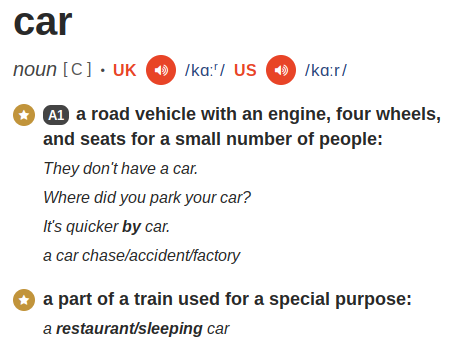
\includegraphics[width=0.37\textwidth]{ch05-cambridge-definition}
      \caption{Example of an HTML page from the Cambridge dictionary.}
      \label{fig:cambrige}
    \end{figure}

    \noindent \texttt{dict2vec} does not focus on learning a vector for each
    sense of polysemous words so the definitions of all the senses of a word are
    concatenated and considered as a single definition. For each word, its
    definitions from all the dictionaries are also concatenated. Stop words and
    punctuation are removed, words are lowercased and a pre-processing step is
    applied to transform plural words to singular ones. For the word ``car'',
    the definition obtained is:

    \begin{quote}
      \small
      \textbf{car}: road vehicle engine wheel seat small number people part
      train special purpose separate part train passenger sit part train
      carrying good animal road vehicle engine wheel seating people car part
      train abbreviation capital adequacy ratio automobile vehicle running rail
      streetcar railroad car part elevator balloon modern airship carries
      passenger freight british wheeled vehicle farm cart wagon
      literary chariot war triumph archaic cart carriage selfpropelled road
      vehicle designed carry passenger wheel powered engine modifier
      conveyance passenger freight cable car carrier airship balloon railway
      vehicle passenger sleeping car buffet car railway carriage van enclosed
      platform lift
    \end{quote}

    \noindent Among the 2.2M unique words, only 200K have a definition. Strong
    and weak pairs are generated from the downloaded definitions according to
    the rules described in~\autoref{ch05:subsec:strong-weak-pairs}, leading to
    417K strong pairs (when the number of close neighbors used to extend strong
    pairs is set to 5) and 3.9M weak pairs.

  \subsection{Training settings}
    \label{ch05:subsec:training-settings}
    \subsubsection{Training corpora}
      \label{ch05:subsubsec:training-corpora}
      \texttt{dict2vec} model is trained with the generated strong and weak
      pairs and the November 2016 English dump from Wikipedia. After removing
      all XML tags found in the Wikipedia dump and converting all words to
      lowercase (with the help of Mahoney's
      script\footnote{\url{http://mattmahoney.net/dc/textdata.html\#appendixa}}),
      the corpus is separated into 3 training files containing respectively the
      first 50M tokens, the first 200M tokens, and the full dump.
      \texttt{dict2vec} uses additional knowledge during training so it would
      not be fair to compare \texttt{dict2vec} to other common models which only
      train word embeddings with a text corpus and no additional knowledge. To
      overcome this shortcoming and have a fair comparison against other models,
      the additional information extracted from definitions is also incorporated
      into the text corpora and two versions of each text training file are
      created: one containing only text from Wikipedia (noted as ``Wikipedia''
      in~\autoref{ch05:sec:results}) and another one with text from Wikipedia
      concatenated to the extracted definitions (noted as ``Wikipedia \texttt{+}
      definitions'' in~\autoref{ch05:sec:results}).

    \subsubsection{Hyperparameters of \texttt{dict2vec}}
      \label{ch05:subsubsec:hyperparameters}
      Hyperparameters for the general settings of \texttt{dict2vec} are set to
      the ones usually found in the literature, that is: $5$ negatives samples,
      $5$ training epochs, a context window composed of $5$ words, a vector size
      of $100$ dimensions (resp. $200$ and $300$) for the 50M tokens
      training file (resp. the 200M tokens and the full dump training files) and
      words with less than $5$ occurrences are removed from the corpus. For the
      specific hyperparameters of \texttt{dict2vec}, the same tuning protocol as
      in the \texttt{word2vec} and \texttt{fasttext} papers is followed to
      provide the fairest comparison against other competitors, so every other
      hyperparameters ($\beta_{s}$, $\beta_{w}$, $n_s$, $n_w$) are tuned with a
      grid search to maximize the weighted average score on a word semantic
      similarity task. For $n_s$ and $n_w$, values from 0 to 10 with a step of 1
      have been tested. For $\beta_{s}$ and $\beta_{w}$, values from 0 to 2 with
      a step of 0.05 have been tested. The optimal hyperparameters for the
      \texttt{dict2vec} model are: $n_s = 4$, $n_w = 5$, $\beta_{s} = 0.8$ and
      $\beta_{w} = 0.45$.

  \subsection{Evaluation protocol}
    \label{ch05:subsec:evaluation-protocol}
    \subsubsection{Evaluation tasks}
      \begin{itemize}
        \item \textbf{Word semantic similarity evaluation.} \texttt{dict2vec}
          follows the standard method for this evaluation task by computing the
          Spearman's rank correlation coefficient \citep{spearman1904proof}
          between human similarity evaluation of pairs of words and the cosine
          similarity of the corresponding word vectors. This task has been
          explained in more details in
          \autoref{ch01:subsubsec:semantic-similarity} of
          \autoref{chap:preliminaries}. The following classic datasets are used:
          \begin{itemize}
            \item MC-30 \citep{miller1991contextual}
            \item MEN \citep{bruni2014multimodal}
            \item MTurk-287 \citep{radinsky2011word}
            \item MTurk-771 \citep{halawi2012large}
            \item RG-65 \citep{rubenstein1965contextual}
            \item RW \citep{luong2013better}
            \item SimVerb-3500 \citep{gerz2016simverb}
            \item WordSim-353 \citep{finkelstein2001placing}
            \item YP-130 \citep{yang2006verb}
          \end{itemize}
          The same protocol as the one used by \texttt{word2vec} and
          \texttt{fasttext} is followed: pairs containing a word which does not
          occur in the training text corpus are discarded. Since
          \texttt{dict2vec} and the competitor models are all trained on the
          same corpora, they all have the same out-of-vocabulary (OOV) rate (the
          ratio of pairs not used to compute the Spearman's rank correlation
          coefficient). Each training is repeated 3 times
          and~\autoref{ch05:tab:results-semantic} reports the average score of
          the 3 training, to minimize the effect of the neural network random
          initialization. The weighted average score (\textit{W.Average}) on all
          datasets is computed by weighting each dataset score by the number of
          pairs that are evaluated in it, in the same way
          as~\citeauthor{iacobacci2016embeddings}~\citep{iacobacci2016embeddings}.

        \item \textbf{Text classification evaluation.} This task (described in
          more details in \autoref{ch01:subsubsec:text-classification-task} in
          \autoref{chap:preliminaries}) follows the same setup as in the
          \texttt{fasttext} paper~\citep{joulin2016bag}. A neural network
          composed of a single hidden layer is trained, where the input layer
          corresponds to the Bag-of-Words of a document and the output layer is
          the probability to belong to each possible class. Weights between the
          input and the hidden layer are initialized with the learned word
          embeddings and are freezed during the neural network training so that
          the evaluation score solely depends on the word embeddings used for
          the initialization. The weights of the neural network are learned with
          the stochastic gradient descent technique to minimize the number of
          prediction errors. The datasets used for this classification task are:
          AG-News\footnote{\url{https://www.di.unipi.it/~gulli/AG_corpus_of_news_articles.html}},
          DBpedia~\citep{auer2007dbpedia} and Yelp
          reviews\footnote{\url{https://www.yelp.com/dataset}} (polarity and
          full). Each dataset is split into a training and a test file. The
          same training and test files are used for all models. The
          classification accuracy obtained on the test file is reported
          in~\autoref{ch05:tab:results-classification}.
      \end{itemize}

    \subsubsection{Baselines}
      Two other models are used to compare the performances of \texttt{dict2vec}
      against competitors:
      \texttt{word2vec}\footnote{\url{https://github.com/tmikolov/word2vec}} and
      \texttt{fasttext}\footnote{\url{https://github.com/facebookresearch/fastText}}.
      Both competitors have been trained on the same 3 corpora as
      \texttt{dict2vec} (50M tokens, 200M tokens and full Wikipedia dump) and
      their 2 respective versions (``Wikipedia'' and ``Wikipedia \texttt{+}
      definitions'' ) described in~\autoref{ch05:subsubsec:training-corpora}.
      They use the same general hyperparameters as \texttt{dict2vec}, which are
      detailed in~\autoref{ch05:subsubsec:hyperparameters} and commonly used in
      the literature. \texttt{word2vec} is trained with its Skip-gram
      architecture because the \texttt{dict2vec} method is based on the
      Skip-gram model. \texttt{GloVe} has also been trained on the same corpora
      with its respective hyperparameters described
      in~\citep{pennington2014glove} but their results are lower than all the
      other baselines (weighted averages on the word semantic similarity task
      are $0.350$ for the 50M file, $0.389$ for the 200M file and $0.454$ for
      the full dump) so the results of \texttt{GloVe} are not reported
      in~\autoref{ch05:tab:results-semantic}.\medskip

      To compare \texttt{dict2vec} against another method which uses additional
      information, word embeddings learned on the ``Wikipedia'' corpus are
      retrofitted with the method of ~\cite{faruqui2015retrofitting}.
      \texttt{retrofitting} introduces external knowledge from the WordNet
      semantic lexicon~\citep{miller1995wordnet}. Word embeddings learned with
      \texttt{dict2vec} and the other competitors are all
      retrofitted\footnote{\url{https://github.com/mfaruqui/retrofitting}} with
      the $\text{WN}_{all}$ semantic lexicon from WordNet and $10$ iterations,
      as advised in the paper of~\citeauthor{faruqui2015retrofitting}. Another
      comparison is made by evaluating the performances of \texttt{dict2vec}
      using WordNet as an additional resource instead of dictionaries.

\section{Results and model analysis}
  \label{ch05:sec:results}
  This section presents the results obtained by the word embeddings learned with
  the \texttt{dict2vec} model on two different tasks: a word semantic similarity
  task (\autoref{ch05:subsec:results-semantic}) and a text classification task
  (\autoref{ch05:subsec:results-classification}). In addition to comparing
  \texttt{dict2vec} to other common methods used to learn word vectors, a
  comparison to a method which improves the captured semantic information with
  additional external knowledge is presented
  in~\autoref{ch05:subsec:dict2vec-vs-retrofitting}. Moreover, a comparison
  between the use of dictionaries and the use of WordNet in the
  \texttt{dict2vec} architecture is presented in
  \autoref{ch05:subsec:dictionaries-vs-wordnet}. Finally,
  \autoref{ch05:subsec:d2v-hyperparameters} analyzes the influence of the
  different hyperparameters of \texttt{dict2vec}.

  \subsection{Word semantic similarity}
    \label{ch05:subsec:results-semantic}

    \autoref{ch05:tab:results-semantic} reports the Spearman's rank correlation
    scores obtained on several datasets and following the protocol described
    in~\autoref{ch05:subsec:evaluation-protocol} for the word semantic
    similarity task. Each model (\texttt{word2vec}, \texttt{fasttext} and
    \texttt{dict2vec}) have been trained on 3 different corpora sizes: 50M
    tokens, 200M tokens and the full Wikipedia dump (which contains around 4.1B
    tokens). Since all the models are trained on the same corpora, the
    percentage of out-of-vocabulary (OOV) pairs (a pair of words in a similarity
    dataset where one of the word is not in the training corpus) is the same for
    all the models. The ratio of OOV pairs for each dataset is reported
    in~\autoref{ch05:tab:oov}. All the pairs have words within the training
    corpora except for the RW dataset, which is expected because this dataset
    contains many Rare Words (RW) which are only found in large corpora (like
    the full Wikipedia dump).

    % table to compare OOV rates with different corpus sizes
    \begin{table}[h]
      \centering
      \begin{tabular}{lccc}
                    & 50M & 200M & full\\
        \toprule[0.1em]
          MC-30     & 0\% & 0\%  & 0\% \\
          MEN-TR-3k & 0\% & 0\%  & 0\% \\
          MTurk-287 & 0\% & 0\%  & 0\% \\
          MTurk-771 & 0\% & 0\%  & 0\% \\
          RG-65     & 0\% & 0\%  & 0\% \\
          RW        & 36\%& 16\% & 2\% \\
          SimVerb   & 3\% & 0\%  & 0\% \\
          WS353-ALL & 0\% & 0\%  & 0\% \\
          WS353-REL & 0\% & 0\%  & 0\% \\
          WS353-SIM & 0\% & 0\%  & 0\% \\
          YP-130    & 3\% & 0\%  & 0\% \\
        \bottomrule[0.1em]
      \end{tabular}
      \caption[Percentage of pairs of words not evaluated in the semantic
      similary task.]{Percentage of pairs of words not used for evaluation in
      the semantic similarity task for different sizes of corpus files and
      datasets. When a pair contains a word not in the vocabulary of the corpus,
      it is discarded for the evaluation.}
      \label{ch05:tab:oov}
    \end{table}

    % Table of word semantic similarity scores
    \begin{table}
      \begin{subtable}{\textwidth} % 50M corpus
        \centering
        % 8 columns (1 + 3 + 1 + 3):
        %   - dataset
        %   - 3 models on Wikipedia
        %   - 1 blank column
        %   - 3 models on Wikipedia+definitions
        \resizebox{0.88\textwidth}{!}{
        \begin{tabular}{@{}lccccccc@{}}
          & \multicolumn{3}{c}{Wikipedia} &&
            \multicolumn{3}{c}{Wikipedia \texttt{+} definitions}\\
          % \cmidrule command of booktabs allows for an optional argument using
          % parentheses ( ) to specify on which side it should be reduced.
          \cmidrule(lr){2-4} \cmidrule(l){6-8}
          & \texttt{word2vec} & \texttt{fasttext} & \texttt{dict2vec} &
          & \texttt{word2vec} & \texttt{fasttext} & \texttt{dict2vec}\\
          \midrule[0.1em]
            %                     w2v     FT       our
            MC-30              & 0.697 & 0.722 & 0.840 &
                               & 0.847 & 0.823 & \bf{0.859}\\
            MEN-TR-3k          & 0.692 & 0.697 & 0.733 &
                               & 0.753 & \bf{0.767} & 0.762\\
            MTurk-287          & 0.657 & 0.657 & 0.665 &
                               & \bf{0.688} & 0.685 & 0.682\\
            MTurk-771          & 0.596 & 0.597 & 0.685 &
                               & 0.677 & 0.692 & \bf{0.713}\\
            RG-65              & 0.714 & 0.671 & 0.824 &
                               & 0.865 & 0.842 & \bf{0.875}\\
            RW                 & 0.375 & 0.442 & 0.475 &
                               & 0.420 & \bf{0.512} & 0.489\\
            SimVerb            & 0.165 & 0.179 & 0.363 &
                               & 0.371 & 0.374 & \bf{0.432}\\
            WS353-ALL          & 0.660 & 0.657 & 0.738 &
                               & 0.739 & 0.739 & \bf{0.753}\\
            WS353-REL          & 0.619 & 0.623 & 0.679 &
                               & \bf{0.700} & 0.696 & 0.688\\
            WS353-SIM          & 0.714 & 0.714 & 0.774 &
                               & \bf{0.797} & 0.790 & 0.784\\
            YP-130             & 0.458 & 0.415 & 0.666 &
                               & 0.679 & 0.674 & \bf{0.696}\\
            \cmidrule(l){2-8}
            \textit{W.Average} & 0.453 & 0.467 & 0.564 &
                               & 0.562 & 0.582 & \bf{0.599}\\
          \bottomrule[0.1em]
        \end{tabular}}
        \caption{Trained with a Wikipedia corpus file of 50M tokens.}
        \vspace*{1em} % to add vertical space between subtables
      \end{subtable}
      \begin{subtable}{\textwidth} % 200M corpus
        \centering
        \resizebox{0.88\textwidth}{!}{
        \begin{tabular}{@{}lccccccc@{}}
          & \multicolumn{3}{c}{Wikipedia} &&
            \multicolumn{3}{c}{Wikipedia \texttt{+} definitions}\\
          \cmidrule(lr){2-4} \cmidrule(l){6-8}
          & \texttt{word2vec} & \texttt{fasttext} & \texttt{dict2vec} &
          & \texttt{word2vec} & \texttt{fasttext} & \texttt{dict2vec}\\
          \midrule[0.1em]
            %                     w2v     FT         our
            MC-30              & 0.742 & 0.795 & \bf{0.854} &
                               & 0.830 & 0.814 & 0.827\\
            MEN-TR-3k          & 0.734 & 0.754 & 0.752 &
                               & 0.758 & \bf{0.772} & 0.768\\
            MTurk-287          & 0.642 & 0.671 & 0.667 &
                               & \bf{0.671} & 0.661 & 0.666\\
            MTurk-771          & 0.628 & 0.632 & 0.682 &
                               & 0.669 & 0.675 & \bf{0.704}\\
            RG-65              & 0.771 & 0.755 & 0.857 &
                               & 0.842 & 0.829 & \bf{0.877}\\
            RW                 & 0.377 & 0.475 & 0.467 &
                               & 0.408 & \bf{0.507} & 0.478\\
            SimVerb            & 0.183 & 0.206 & 0.377 &
                               & 0.306 & 0.329 & \bf{0.424}\\
            WS353-ALL          & 0.694 & 0.701 & \bf{0.762} &
                               & 0.734 & 0.735 & 0.758\\
            WS353-REL          & 0.665 & 0.644 & \bf{0.710} &
                               & 0.706 & 0.685 & 0.699\\
            WS353-SIM          & 0.743 & 0.758 & 0.784 &
                               & \bf{0.792} & 0.792 & 0.787\\
            YP-130             & 0.449 & 0.509 & 0.616 &
                               & 0.592 & 0.639 & \bf{0.665}\\
            \cmidrule{2-8}
            \textit{W.Average} & 0.471 & 0.503 & 0.569 &
                               & 0.533 & 0.563 & \bf{0.592}\\
          \bottomrule[0.1em]
        \end{tabular}}
        \caption{Trained with a Wikipedia corpus file of 200M tokens.}
        \vspace*{1em}
      \end{subtable}
      \begin{subtable}{\textwidth} % full dump
        \centering
        \resizebox{0.88\textwidth}{!}{
        \begin{tabular}{@{}lccccccc@{}}
          & \multicolumn{3}{c}{Wikipedia} &&
            \multicolumn{3}{c}{Wikipedia \texttt{+} definitions}\\
          \cmidrule(lr){2-4} \cmidrule(l){6-8}
          & \texttt{word2vec} & \texttt{fasttext} & \texttt{dict2vec} &
          & \texttt{word2vec} & \texttt{fasttext} & \texttt{dict2vec}\\
          \midrule[0.1em]
            %                     w2v     FT         our
            MC-30              & 0.809 & 0.831 & \bf{0.860} &
                               & 0.826 & 0.815 & 0.847 \\
            MEN-TR-3k          & 0.733 & 0.752 & \bf{0.756} &
                               & 0.728 & 0.751 & 0.755 \\
            MTurk-287          & 0.660 & \bf{0.672} & 0.661 &
                               & 0.656 & 0.671 & 0.660 \\
            MTurk-771          & 0.623 & 0.631 & \bf{0.696} &
                               & 0.620 & 0.638 & 0.694 \\
            RG-65              & 0.787 & 0.817 & \bf{0.875} &
                               & 0.802 & 0.820 & 0.867 \\
            RW                 & 0.407 & 0.464 & \bf{0.482} &
                               & 0.427 & 0.468 & 0.476 \\
            SimVerb            & 0.186 & 0.222 & \bf{0.384} &
                               & 0.214 & 0.233 & 0.379 \\
            WS353-ALL          & 0.705 & 0.729 & 0.756 &
                               & 0.721 & 0.723 & \bf{0.758} \\
            WS353-REL          & 0.664 & 0.687 & 0.702 &
                               & 0.681 & 0.686 & \bf{0.703} \\
            WS353-SIM          & 0.757 & 0.775 & 0.781 &
                               & 0.767 & 0.779 & \bf{0.781} \\
            YP-130             & 0.502 & 0.533 & \bf{0.646} &
                               & 0.475 & 0.553 & 0.607 \\
            \cmidrule{2-8}
            \textit{W.Average} & 0.476 & 0.508 & \bf{0.573} &
                               & 0.488 & 0.512 & 0.570 \\
          \bottomrule[0.1em]
        \end{tabular}}
        \caption{Trained with the full Wikipedia corpus file.}
      \end{subtable}
      \caption[Evaluation of \texttt{dict2vec} and other models on a semantic
      similarity task.]{Semantic similarity scores on several datasets and
      different sizes of corpora for \texttt{word2vec}, \texttt{fasttext} and
      \texttt{dict2vec}. Each model is trained and evaluated 3 times; the mean
      score of the 3 runs is reported in the table. \textit{W.average} is the
      weighted average for all word similarity datasets.}
      \label{ch05:tab:results-semantic}
    \end{table}

    \paragraph{\texttt{dict2vec} vs. others.}
      The \texttt{dict2vec} model outperforms other approaches on most of the
      datasets for the 50M and the 200M tokens files, and on all datasets
      (excepted one) for the full Wikipedia dump (this is significant according
      to a two-sided Wilcoxon signed-rank test with $\alpha=0.05$). On the
      weighted average score, the \texttt{dict2vec} model improves
      \texttt{fasttext} performances on the ``Wikipedia'' corpus by $20.8\%$ for
      the 50M tokens file, by $13.1\%$ for the 200M tokens file and by $12.8\%$
      for the full dump. Even when \texttt{fasttext} has access to additional
      knowledge during training (scores in the column ``Wikipedia \texttt{+}
      definitions''), the \texttt{dict2vec} model still has better performances
      with an increase of $2.9\%$ for the 50M tokens file, $5.2\%$ for the 200M
      tokens file and $11.3\%$ for the full dump.

      Models based on external knowledge sources presented
      in~\autoref{ch03:sec:external-resources} of~\autoref{chap:methods-we} do
      not provide word semantic similarity scores for all the datasets used in
      this evaluation. However, for the reported scores, \texttt{dict2vec}
      outperforms these
      models:~\citeauthor{kiela2015specializing}~\citep{kiela2015specializing}
      reach a score of $0.72$ on the MEN dataset ($0.756$ for
      \texttt{dict2vec});~\citeauthor{xu2014rc}~\citep{xu2014rc} obtain $0.683$
      on the WS353-ALL dataset ($0.758$ for \texttt{dict2vec}).

    \paragraph{Adding definitions to the corpus.}
      The column ``Wikipedia \texttt{+} definitions''
      in~\autoref{ch05:tab:results-semantic}, which represents the case where
      training corpora are composed of Wikipedia and word definitions
      concatenated to them, has better results than the column ``Wikipedia''
      which represents training corpora only composed of Wikipedia: $+18.3\%$ on
      average for the 50M tokens file, $+9.7\%$ for the 200M tokens file. This
      demonstrates the strong semantic relations one can find in definitions and
      that simply incorporating definitions into small training corpora can
      boost the performances of the word embeddings trained on them. This is
      significant because the training time is largely decreased when the corpus
      file is smaller (training with the 50M tokens corpus file is 150 times
      faster than training on the full Wikipedia corpus) so adding definitions
      is a better option than extending the corpus with content from Wikipedia.
      However, when the training file is large (full dump), the supervision
      brought by strong and weak pairs is more efficient to improve the word
      semantic similarity scores than adding word definitions to the corpus as
      the boost brought by the concatenation of definitions is not significant
      for the full dump ($+0.9\%$ on average). It is also important to observe
      that, although the \texttt{dict2vec} model is superior for each corpus
      size, its word embeddings trained on the ``Wikipedia'' corpus of 50M
      tokens outperforms the word embeddings of other models trained on the
      ``Wikipedia'' full dump (an improvement of $11\%$ compared to the results
      of \texttt{fasttext} vectors, its best competitor, trained on the full
      dump). This means that considering strong and weak pairs in a model is
      more efficient than increasing the training corpus size and that using
      dictionaries is a good way to improve the quality of the embeddings when
      the training file is small.

  \subsection{Text classification accuracy}
    \label{ch05:subsec:results-classification}

    % Table of text classification scores
    \begin{table}[!t]
      \begin{subtable}{\textwidth}
        \centering
        \resizebox{0.85\textwidth}{!}{
        \begin{tabular}{@{}lccccccc@{}}
          & \multicolumn{3}{c}{Wikipedia} &&
            \multicolumn{3}{c}{Wikipedia \texttt{+} definitions}\\
          \cmidrule(lr){2-4} \cmidrule(l){6-8}
          & \texttt{word2vec} & \texttt{fasttext} & \texttt{dict2vec} &
          & \texttt{word2vec} & \texttt{fasttext} & \texttt{dict2vec}\\
          \midrule[0.1em]
            %            w2v     FT         our
            AG-News   & \bf{87.4} & 86.8 & 87.1 &
                      & 87.1 & 87.1 & 86.6\\
            DBPedia   & 93.5 & 94.2 & \bf{94.4} &
                      & 94.2 & 94.4 & 94.4\\
            Yelp Pol. & 80.8 & 82.1 & 83.2 &
                      & 83.5 & \bf{84.2} & 83.4\\
            Yelp Full & 45.1 & 46.0 & 47.1 &
                      & 46.9 & \bf{47.3} & 47.2\\
          \bottomrule[0.1em]
        \end{tabular}}
        \caption{Trained with a Wikipedia corpus file of 50M tokens.}
        \vspace*{1em}
      \end{subtable}
      \begin{subtable}{\textwidth}
        \centering
        \resizebox{0.85\textwidth}{!}{
        \begin{tabular}{@{}lccccccc@{}}
          & \multicolumn{3}{c}{Wikipedia} &&
            \multicolumn{3}{c}{Wikipedia \texttt{+} definitions}\\
          \cmidrule(lr){2-4} \cmidrule(l){6-8}
          & \texttt{word2vec} & \texttt{fasttext} & \texttt{dict2vec} &
          & \texttt{word2vec} & \texttt{fasttext} & \texttt{dict2vec}\\
          \midrule[0.1em]
            %            w2v     FT         our
            AG-News   & \bf{88.6} & 88.0 & 88.0 &
                      & 88.2 & 88.1 & 88.0\\
            DBPedia   & 95.2 & 95.7 & \bf{96.0} &
                      & 95.6 & 95.8 & 95.9\\
            Yelp Pol. & 83.7 & 85.2 & 85.6 &
                      & 85.5 & 85.9 & \bf{85.9}\\
            Yelp Full & 47.7 & 48.8 & 49.9 &
                      & 49.1 & 49.5 &\bf{50.1}\\
          \bottomrule[0.1em]
        \end{tabular}}
        \caption{Trained with a Wikipedia corpus file of 200M tokens.}
        \vspace*{1em}
      \end{subtable}
      \begin{subtable}{\textwidth}
        \centering
        \resizebox{0.85\textwidth}{!}{
        \begin{tabular}{@{}lccccccc@{}}
          & \multicolumn{3}{c}{Wikipedia} &&
            \multicolumn{3}{c}{Wikipedia \texttt{+} definitions}\\
          \cmidrule(lr){2-4} \cmidrule(l){6-8}
          & \texttt{word2vec} & \texttt{fasttext} & \texttt{dict2vec} &
          & \texttt{word2vec} & \texttt{fasttext} & \texttt{dict2vec}\\
          \midrule[0.1em]
            %            w2v     FT         our
            AG-News   & 88.5 & \bf{88.7} & 88.1 &
                      & 88.5 & 88.7 & 88.4\\
            DBPedia   & 96.6 & 96.7 & 96.8 &
                      & 96.6 & 96.7 & \bf{96.9}\\
            Yelp Pol. & 86.5 & 87.2 & \bf{87.6} &
                      & 86.7 & 87.4 & 87.5\\
            Yelp Full & 50.6 & 51.2 & 51.6 &
                      & 50.6 & 51.4 & \bf{51.8}\\
          \bottomrule[0.1em]
        \end{tabular}}
        \caption{Trained with the full Wikipedia corpus file.}
      \end{subtable}
      \caption[Evaluation of \texttt{dict2vec} and other models on a text
      classification task.]{Accuracies on a text classification task (percentage
      of correctly classified documents). Each model is trained and evaluated 3
      times; the mean score of the 3 runs is reported.}
      \label{ch05:tab:results-classification}
    \end{table}

    \autoref{ch05:tab:results-classification} reports the classification
    accuracies (percentage of correctly classified documents) obtained for
    \texttt{word2vec}, \texttt{fasttext} and \texttt{dict2vec} on the datasets
    listed in~\autoref{ch05:subsec:evaluation-protocol}. The \texttt{dict2vec}
    model achieves similar level of performances as \texttt{word2vec} and
    \texttt{fasttext} when trained on the 50M tokens file and slightly better
    results when trained on the 200M tokens file and on the full dump. Using
    strong and weak pairs as a supervision during training does not make the
    \texttt{dict2vec} model specialized for the word semantic similarity task,
    which demonstrates that the learned embeddings can also be used in
    downstream models for extrinsic tasks. In this classification evaluation,
    values of the embeddings are not updated during the training
    phase (only the parameters of the classifier are learned)
    since the objective is to evaluate the capacity of the embeddings to be used
    in another task rather than obtaining the best possible classification
    model. It is however possible to obtain better results than those presented
    in~\autoref{ch05:tab:results-classification} by updating the embeddings
    values during training with the supervised information of labeled documents
    in order to adapt the embeddings for this classification task, as done
    by~\citeauthor{joulin2016bag}~\citep{joulin2016bag}.

  \subsection{\texttt{dict2vec} vs. \texttt{retrofitting}}
    \label{ch05:subsec:dict2vec-vs-retrofitting}

    % Table to compare the score of retrofitted vectors and original d2v vectors
    \begin{table}[h]
      \centering
      \resizebox{\textwidth}{!}{
        \begin{tabular}{@{}lcccccccccccc@{}} % all 13 columns are centered,
                                             % except 1st one that left aligned
        &
        & \multicolumn{3}{c}{50M} & \phantom{}
        & \multicolumn{3}{c}{200M} & \phantom{}
        & \multicolumn{3}{c}{full}\\
        \cmidrule{3-5} \cmidrule{7-9} \cmidrule{11-13}
          && \texttt{w2v}\indic{rf} & \texttt{ft}\indic{rf} & \texttt{d2v}\indic{rf}
          && \texttt{w2v}\indic{rf} & \texttt{ft}\indic{rf} & \texttt{d2v}\indic{rf}
          && \texttt{w2v}\indic{rf} & \texttt{ft}\indic{rf} & \texttt{d2v}\indic{rf}\\
        \midrule[0.1em]
        %    w2v           FT         d2v
        \multirow{2}{*}{MC-30}
          &vs. self (not \teal{rf}) &
                +13.9\% &      +9.2\% & +1.3\% &&
                 +5.8\% &      +4.8\% & +3.0\% &&
                 +5.2\% &      +2.9\% & +1.2\% \\
          &vs. \texttt{d2v} (not \teal{rf}) &
            \bf{-7.3\%} & \bf{-4.4\%} &    $-$ &&
            \bf{-3.6\%} & \bf{-2.4\%} &    $-$ &&
            \bf{-1.0\%} & \bf{-0.6\%} &    $-$ \\
        \cmidrule{2-13}
        \multirow{2}{*}{MEN-TR-3k}
          &vs. self (not \teal{rf}) &
                 +0.9\% &      -0.7\% & -0.1\% &&
                 +0.7\% &      -1.9\% & +0.4\% &&
                 +1.4\% &      -2.8\% & +1.6\% \\
          &vs. \texttt{d2v} (not \teal{rf}) &
            \bf{-4.2\%} & \bf{-7.4\%} &    $-$ &&
            \bf{-1.3\%} & \bf{-1.6\%} &    $-$ &&
            \bf{-1.7\%} & \bf{-3.3\%} &    $-$ \\
        \cmidrule{2-13}
        \multirow{2}{*}{MTurk-287}
          &vs. self (not \teal{rf}) &
                 +1.4\% &      +0.2\% & +3.5\% &&
                 -2.9\% &      -3.3\% & +3.0\% &&
                 -0.9\% &      -5.7\% & +1.1\% \\
          &vs. \texttt{d2v} (not \teal{rf}) &
            \bf{-1.2\%} & \bf{-4.0\%} &    $-$ &&
            \bf{-4.3\%} & \bf{-2.7\%} &    $-$ &&
            \bf{-1.1\%} & \bf{-4.1\%} &    $-$ \\
        \cmidrule{2-13}
        \multirow{2}{*}{MTurk-771}
          &vs. self (not \teal{rf}) &
                 +8.2\% &      +4.9\% & +1.6\% &&
                 +6.3\% &      +4.3\% & +1.5\% &&
                 +4.5\% &      +1.6\% & +0.6\% \\
          &vs. \texttt{d2v} (not \teal{rf}) &
            \bf{-7.3\%} & \bf{-8.8\%} &    $-$ &&
            \bf{-3.8\%} & \bf{-3.4\%} &    $-$ &&
            \bf{-6.5\%} & \bf{-7.9\%} &    $-$ \\
        \cmidrule{2-13}
        \multirow{2}{*}{RG-65}
          &vs. self (not \teal{rf}) &
                +10.9\% &     +17.1\% & +4.0\% &&
                 +6.6\% &      +8.5\% & +3.0\% &&
                 +7.0\% &      +5.0\% & +2.4\% \\
          &vs. \texttt{d2v} (not \teal{rf}) &
            \bf{-2.1\%} & \bf{-4.9\%} &    $-$ &&
            \bf{-2.2\%} & \bf{-4.4\%} &    $-$ &&
            \bf{-3.8\%} & \bf{-1.9\%} &    $-$ \\
        \cmidrule{2-13}
        \multirow{2}{*}{RW}
          &vs. self (not \teal{rf}) &
                 -20.3\% &    -24.4\% & -14.3\% &&
                 -24.4\% &    -25.9\% & -20.3\% &&
                 -18.7\% &    -25.4\% & -19.1\% \\
          &vs. \texttt{d2v} (not \teal{rf}) &
            \bf{-37.4\%} & \bf{-26.9\%} &   $-$ &&
            \bf{-37.7\%} & \bf{-24.6\%} &   $-$ &&
            \bf{-31.3\%} & \bf{-28.2\%} &   $-$ \\
        \cmidrule{2-13}
        \multirow{2}{*}{Simverb}
          &vs. self (not \teal{rf}) &
                 +46.0\% &      +34.0\% & +19.8\% &&
                 +49.7\% &      +39.8\% & +19.9\% &&
                 +44.6\% &      +38.7\% & +16.7\% \\
          &vs. \texttt{d2v} (not \teal{rf}) &
            \bf{-34.4\%} & \bf{-28.4\%} &     $-$ &&
            \bf{-30.5\%} & \bf{-23.6\%} &     $-$ &&
            \bf{-29.9\%} & \bf{-19.8\%} &     $-$ \\
        \cmidrule{2-13}
        \multirow{2}{*}{WS353-ALL}
          &vs. self (not \teal{rf}) &
                  -4.2\% &     -10.8\% & -1.1\% &&
                  -3.2\% &      -8.0\% & -1.3\% &&
                  -4.4\% &     -10.7\% & -2.0\% \\
          &vs. \texttt{d2v} (not \teal{rf}) &
            \bf{-13.8\%} &\bf{-19.2\%} &    $-$ &&
            \bf{-11.9\%} &\bf{-15.4\%} &    $-$ &&
            \bf{-10.8\%} &\bf{-13.9\%} &    $-$ \\
        \cmidrule{2-13}
        \multirow{2}{*}{WS353-REL}
          &vs. self (not \teal{rf}) &
                 -16.1\% &     -22.7\% & -4.9\% &&
                 -10.4\% &     -17.9\% & -4.5\% &&
                 -10.7\% &     -19.7\% & -6.0\% \\
          &vs. \texttt{d2v} (not \teal{rf}) &
            \bf{-20.9\%} &\bf{-27.2\%} &    $-$ &&
            \bf{-17.7\%} &\bf{-25.5\%} &    $-$ &&
            \bf{-15.5\%} &\bf{-21.4\%} &    $-$ \\
        \cmidrule{2-13}
        \multirow{2}{*}{WS353-SIM}
          &vs. self (not \teal{rf}) &
                 +4.3\% &      +0.8\% & +3.2\% &&
                 +2.6\% &      +0.0\% & +3.2\% &&
                 +0.0\% &      -3.6\% & +2.4\% \\
          &vs. \texttt{d2v} (not \teal{rf}) &
            \bf{-3.9\%} & \bf{-6.7\%} &    $-$ &&
            \bf{-2.9\%} & \bf{-3.3\%} &    $-$ &&
            \bf{-3.0\%} & \bf{-4.4\%} &    $-$ \\
        \cmidrule{2-13}
        \multirow{2}{*}{YP-130}
          &vs. self (not \teal{rf}) &
                 +17.8\% &      +3.2\% & +3.3\% &&
                 +13.0\% &      +6.9\% & +8.0\% &&
                 +11.1\% &      +8.3\% & +5.0\% \\
          &vs. \texttt{d2v} (not \teal{rf}) &
            \bf{-23.6\%} &\bf{-28.2\%} &    $-$ &&
            \bf{-16.6\%} &\bf{-11.7\%} &    $-$ &&
            \bf{-13.6\%} &\bf{-10.7\%} &    $-$ \\
        \bottomrule[0.15em]
      \end{tabular}}
      \caption[Semantic similarity scores differences between
      \texttt{retrofitting} and \texttt{dict2vec}.]{(\teal{rf} = retrofitted).
      Percentage differences of word semantic similarity scores between
      retrofitted vectors (\texttt{X}\indic{rf}) and non-retrofitted vectors
      (not \teal{rf}).  Each model is compared to their own non-retrofitted
      version (vs. self) and \texttt{dict2vec} non-retrofitted version (vs.
      \texttt{d2v}). A positive (resp.  negative) percentage indicates that
      \texttt{retrofitting} improves (resp.  deteriorates) the semantic score
      compared to non-retrofitted vectors.  As an illustration: the top left
      value $+13.9\%$ means that \texttt{word2vec} retrofitted vectors improves
      the initial \texttt{word2vec} vectors performance by $13.9\%$, while the
      value $-7.3\%$ right below it means that their performance is
      $7.3\%$ lower than the non-retrofitted vectors of \texttt{dict2vec}.}
      \label{ch05:tab:results-faruqui}
    \end{table}

    \texttt{retrofitting} \citep{faruqui2015retrofitting} is a method to improve
    the semantic information encoded into word embeddings \textbf{after} they
    have been trained on a corpus (this method is described in more details
    in~\autoref{ch03:sec:external-resources} of~\autoref{chap:methods-we}).
    \citeauthor{faruqui2015retrofitting} method has been applied on each of the
    word embeddings trained on ``Wikipedia'' corpora with pairs of related words
    extracted from WordNet to produce retrofitted vectors of the
    \texttt{word2vec}, \texttt{fasttext} and \texttt{dict2vec} models.
    Retrofitted vectors have been evaluated on the word semantic similarity task
    on all the datatsets and scores of retrofitted vectors are compared to
    either: (i) the score of non-retrofitted vectors for the same model and the
    same corpus size (vs. self (not \teal{rf})); (ii) the score of
    non-retrofitted vectors of \texttt{dict2vec} for the same corpus size (vs.
    \texttt{d2v} (not \teal{rf})). The percentages of score differences are
    reported in~\autoref{ch05:tab:results-faruqui}.\smallskip
    % using a \medskip here fucks up the formatting

    The \texttt{retrofitting} method improves the word semantic similarity
    scores for all models on almost all datasets because the percentages
    differences are almost always positive when retrofitted vectors are compared
    to their non-retrofitted version (``vs. self (not \teal{rf})''
    in~\autoref{ch05:tab:results-faruqui}). However, for the datasets RW,
    WS353-ALL and WS353-REL, the percentages are negative, which indicates that
    \texttt{retrofitting} deteriorates the semantic linguistic information
    encoded into the word embeddings which is needed to evaluate that pairs from
    those datasets are related. While \texttt{retrofitting} can improve the
    quality of information encoded into word embeddings and thus increase the
    scores on the semantic similarity task, it cannot reach the performance
    increase that \texttt{dict2vec} brings. Indeed, even when \texttt{word2vec}
    and \texttt{fasttext} vectors are retrofitted (columns
    \texttt{w2v}\indic{rf} and \texttt{ft}\indic{rf}
    in~\autoref{ch05:tab:results-faruqui}), their scores are still lower than
    the scores of non-retrofitted \texttt{dict2vec} vectors (every percentages
    in the ``vs. \texttt{d2v} (not \teal{rf})'' rows are negative). It can also
    be noticed that \texttt{dict2vec} model is compatible with a retrofitting
    improvement method as its scores are also increased with
    the~\citeauthor{faruqui2015retrofitting} method. \texttt{dict2vec} uses
    additional information from dictionaries while \texttt{retrofitting} uses
    information from WordNet. This demonstrates that the two external sources of
    kwowledge are not overlapping nor exclusive and that a model using both have
    better performances than a model which uses only one of the two.

  \subsection{Dictionaries vs. WordNet}
    \label{ch05:subsec:dictionaries-vs-wordnet}
    \autoref{tab:retrofit-wordnet-dict} reports the weighted average of semantic
    similarity scores of vectors obtained after training (not retrofitted) and
    vectors retrofitted with either pairs from WordNet or pairs generated from
    dictionaries.  Retrofitting with dictionaries pairs outperforms retrofitting
    with WordNet pairs, meaning that information from dictionaries is better
    suited to improve word embeddings towards semantic similarities when
    retrofitting.

    % table to compare retrofitting w/ wordnet vs retrofitting w/ dictionaries
    \begin{table}[h!]
      \centering
      %\small
      \begin{tabular}{ccccc}
        & & not retrofitted & $\text{retrofitted}_{\text{WordNet}}$
                            & $\text{retrofitted}_{\text{dictionaries}}$ \\
        \toprule
        \multirow{3}{*}{50M}
          & \texttt{word2vec} & 0.453 & 0.474 & \bf{0.479} \\
          & \texttt{fasttext} & 0.467 & 0.476 & \bf{0.489} \\
          & \texttt{dict2vec} & 0.569 & 0.582 & \bf{0.582} \\
        \midrule
        \multirow{3}{*}{200M}
          & \texttt{word2vec} & 0.471 & 0.488 & \bf{0.494} \\
          & \texttt{fasttext} & 0.503 & 0.504 & \bf{0.524} \\
          & \texttt{dict2vec} & 0.569 & 0.581 & \bf{0.587} \\
        \midrule
        \multirow{3}{*}{full}
          & \texttt{word2vec} & 0.488 & 0.507 & \bf{0.512} \\
          & \texttt{fasttext} & 0.508 & 0.503 & \bf{0.529} \\
          & \texttt{dict2vec} & 0.571 & 0.583 & \bf{0.592} \\
        \bottomrule
      \end{tabular}
      \caption[Semantic similarity scores when retrofitting with WordNet or
      dictionaries.]{Weighted average of word semantic similarity scores for
      non-retrofitted vectors and after retrofitting vectors with
      WordNet pairs or with dictionary pairs.}
      \label{tab:retrofit-wordnet-dict}
    \end{table}

    To compare the linguistic information one can found in WordNet or in
    dictionaries, the \texttt{dict2vec} model has also been trained without
    using any strong nor weaks pairs during training or by using WordNet pairs
    as strong pairs. When no pairs are used, the \texttt{dict2vec} model is
    equivalent to the \texttt{word2vec} Skip-gram model. Weighted average of
    word semantic scores are reported
    in~\autoref{ch05:tab:training-wordnet-dict}. Training with WordNet pairs
    used as strong pairs increases the scores compared to a model that does not
    use any pairs at all, showing that the supervision brought by the positive
    sampling of \texttt{dict2vec} is beneficial to the model. But it is not as
    good as when the model uses dictionary pairs, demonstrating once again that
    dictionaries contain more semantic information than WordNet.

    % table to compare dict2vec using wordnet pairs vs. dictionary pairs
    \begin{table}[htb]
      \centering
      \begin{tabular}{cccc}
                              &  50M  &  200M & full \\
        \toprule
        No pairs              & 0.453 & 0.471 & 0.488 \\
        With WordNet pairs    & 0.564 & 0.566 & 0.559 \\
        With dictionary pairs & \bf{0.569} & \bf{0.569} & \bf{0.571} \\
        \bottomrule
      \end{tabular}
      \caption[Semantic similarity scores when using pairs from WordNet or
      dictionaries.]{Weighted average semantic similarity scores of
      \texttt{dict2vec} models when trained without pairs and with WordNet or
      dictionary pairs.}
      \label{ch05:tab:training-wordnet-dict}
    \end{table}

  \subsection{Influence of \texttt{dict2vec} hyperparameters}
    \label{ch05:subsec:d2v-hyperparameters}
    \paragraph{Number of strong and weak pairs.}
      The different experiments carried out when training the \texttt{dict2vec}
      model has shown one thing: the number of strong and weak pairs (resp.
      $n_s$ and $n_w$) drawn for each word must be set accordingly to the size
      of the training file. For the 50M and the 200M tokens files, the
      \texttt{dict2vec} model is set with the hyperparameters $n_s = 4$ and $n_w
      = 5$. When training on the full dump (which is 20 times larger than the
      200M tokens file because it contains about 4.1B tokens), the number of
      context windows in the corpus is largely increased, so is the number of
      ($target,~context$) pairs and thus the number of times the positive
      sampling is used for the most frequent words. Therefore, the influence of
      strong and weak pairs needs to be adjusted and decreased because frequent
      words would be learned mainly from their strong and weak pairs not from
      the context windows in which they occur. When trained on the full dump,
      the number of strong and weak pairs used to learn word embeddings are set
      to $n_s = 2$ and $n_w = 3$.

    \paragraph{Weight of strong and weak pairs.}
      For the hyperparameters of the positive sampling, an empirical grid search
      shows that a $\frac{1}{2}$ ratio between $\beta_s$ and $\beta_w$ is a good
      rule-of-thumb for tuning these hyperparameters. It has also been noticed
      that when these coefficients are too low ($\beta_s \leq 0.5$ and $\beta_w
      \leq 0.2$), results get worse because the model does not take into account
      the information from the strong and weak pairs. On the other side, when
      they are too high ($\beta_s \geq 1.2$ and $\beta_w \geq 0.6$), the model
      discards too much information from the context in favor of the information
      from the pairs. This behavior is similar when the number of strong and
      weak pairs is too low or too high ($n_s, n_w \leq 2$ or $n_s, n_w \geq
      5$).

    \paragraph{Number of negative samples.}
      The controlled negative sampling of \texttt{dict2vec} (see
      \autoref{ch05:subsec:controlled-negative-sampling}), which prevents the
      vectors of words forming a strong or a weak pair to be moved apart when
      words are randomly chosen during the negative sampling, increases the
      weighted average semantic similarity scores of learned word embeddings by
      $0.7\%$ compared to the non-controlled version. Increasing the number of
      negative samples used during the training phase does not significantly
      improve the results except on the RW dataset where using 25 negative
      samples can boost the scores by $10\%$, as shown
      in~\autoref{ch05:fig:negative-sampling}. Indeed, this dataset is mostly
      composed of rare words so word embeddings must learn to differentiate
      unrelated words rather than learning which vectors should be moved closer.

      % figure to show evolution of score when number of negative samples change
      \begin{figure}[h]
        \centering
          \begin{tikzpicture}
          \begin{axis}[
              xlabel=Number of negative samples,
              ylabel=Semantic similarity score,
              legend style={at={(0.8,0.5)}, anchor=east, font=\footnotesize}]
            \addplot[color=blue, mark=o] coordinates { % RW-STANFORD
              (1,0.442)
              (3,0.455)
              (5,0.454)
              (7,0.470)
              (9,0.472)
              (11,0.468)
              (13,0.485)
              (15,0.486)
              (17,0.483)
              (19,0.485)
              (21,0.485)
              (23,0.491)
              (25,0.486)
            };
            \addplot[color=red, mark=triangle] coordinates { % WS-353-ALL
              (1,0.731)
              (3,0.746)
              (5,0.750)
              (7,0.751)
              (9,0.747)
              (11,0.746)
              (13,0.744)
              (15,0.737)
              (17,0.741)
              (19,0.744)
              (21,0.739)
              (23,0.743)
              (25,0.736)
            };
            \addplot[color=orange, mark=x] coordinates { % MEN
              (1,0.722)
              (3,0.735)
              (5,0.739)
              (7,0.741)
              (9,0.745)
              (11,0.743)
              (13,0.746)
              (15,0.745)
              (17,0.745)
              (19,0.746)
              (21,0.743)
              (23,0.742)
              (25,0.744)
            };
            \legend{RW, WS353-ALL, MEN-TR-3k}
          \end{axis}
        \end{tikzpicture}
        \caption[Evolution of semantic similarity according to the number of
        negative samples.]{Semantic similarity scores on several datasets (RW,
        WS353-ALL and MEN-TR-3k) when the \texttt{dict2vec} model is trained
        with different numbers of negative samples.}
        \label{ch05:fig:negative-sampling}
      \end{figure}

    \paragraph{Dimensions of word embeddings.}
      Word embeddings with different numbers of dimensions have been trained
      with the \texttt{fasttext} and \texttt{dict2vec} models on the
      ``Wikipedia'' corpus of 50M tokens. Their semantic similarity scores on RW
      and WS353-ALL datasets are reported
      in~\autoref{ch05:fig:dimensions-embeddings}. It can be observed that
      \texttt{dict2vec} is still able to outperform the competitor approach when
      the number of dimensions of vectors is reduced to $20$ or $40$. Moreover,
      increasing the number of dimensions does increase the scores but only up
      to a certain point. When the number of dimensions is higher than 100, no
      significant improvements in semantic similarity scores are observed, which
      supports the fact that other common approaches choose vectors of dimension
      100 when the training corpus is small.

      \begin{figure}[h]
        \centering
          \begin{tikzpicture}
          \begin{axis}[
              xlabel=Number of dimensions of word vectors,
              ylabel=Semantic similarity score,
              legend style={at={(0.96,0.53)}, anchor=east, font=\footnotesize}]
            % fasttext in BLUE, dict2vec in RED
            % RW in circle, WSALL in triangle
            \addplot[color=red, mark=triangle] coordinates { % WS353-ALL - our
              (20,0.680)
              (40,0.736)
              (60,0.746)
              (80,0.740)
              (100,0.731)
              (120,0.750)
              (140,0.739)
              (160,0.744)
              (180,0.743)
              (200,0.749)
            };
            \addplot[color=red, mark=o] coordinates { % RW - our
              (20,0.420)
              (40,0.451)
              (60,0.470)
              (80,0.467)
              (100,0.469)
              (120,0.476)
              (140,0.476)
              (160,0.478)
              (180,0.485)
              (200,0.484)
            };
            \addplot[color=blue, mark=triangle] coordinates { % WS353-ALL - FT
              (20,0.569)
              (40,0.628)
              (60,0.647)
              (80,0.649)
              (100,0.667)
              (120,0.678)
              (140,0.670)
              (160,0.681)
              (180,0.678)
              (200,0.669)
            };
            \addplot[color=blue, mark=o] coordinates { % RW - FT
              (20,0.379)
              (40,0.422)
              (60,0.446)
              (80,0.456)
              (100,0.465)
              (120,0.475)
              (140,0.482)
              (160,0.485)
              (180,0.492)
              (200,0.489)
            };
            \legend{\texttt{dict2vec} - WS353, \texttt{dict2vec} - RW~~~~~,
                    \texttt{fasttext} - WS353, \texttt{fasttext} - RW~~~~~}
          \end{axis}
        \end{tikzpicture}
        \caption[Evolution of semantic similarity according to the size of word
        vectors.]{Semantic similarity scores on the RW and the WS353-ALL datasets
        for \texttt{fasttext} and \texttt{dict2vec} word embeddings trained with
        different numbers of dimensions on the ``Wikipedia'' corpus of 50M
        tokens.}
        \label{ch05:fig:dimensions-embeddings}
      \end{figure}

    \paragraph{Training time.}
      The source code of the \texttt{dict2vec} model is based on the source code
      of the \texttt{word2vec} model, but the majority of the code has been
      rewritten and optimized for a faster training of word embeddings. The
      training times of different models on different corpora sizes are reported
      in~\autoref{ch05:tab:training-times} (all experiments were run on a Intel
      E3-1246 v3 processor). Although \texttt{dict2vec} performs more operations
      during training than the \texttt{word2vec} Skip-gram model (because of the
      additional positive sampling and the controlled negative sampling), it is
      $4$ times faster due to its code optimizations for
      word embeddings learned from the full Wikipedia dump, and almost $3$ times
      as fast as \texttt{fasttext}.

      \begin{table}[h]
        \centering
        \begin{tabular}{lccc}
                            &  50M  & 200M & full \\
        \midrule
          \texttt{word2vec} & 15m30 & 86m  & 2600m \\
          \texttt{fasttext} & 8m44  & 66m  & 1870m \\
          \texttt{dict2vec} & 4m09  & 26m  & 642m \\
        \bottomrule
        \end{tabular}
        \caption[Training time of the \texttt{word2vec}, \texttt{fasttext} and
        \texttt{dict2vec} models.]{Training time (in minutes) of the
        \texttt{word2vec}, \texttt{fasttext} and \texttt{dict2vec} models for
        several corpora sizes.}
        \label{ch05:tab:training-times}
      \end{table}

\section{Conclusion}
  % description rapide de dict2vec modele
  This chapter presented the first contribution of this thesis. As pointed out
  in~\autoref{chap:methods-we}, most of the existing methods to learn word
  embeddings only use generic text corpora like Wikipedia. The model presented
  here, named \texttt{dict2vec}, uses additional information from lexical
  dictionaries during training to encode more linguistic and semantic
  information into word embeddings. It generates pairs of related words (and in
  some cases, pairs of strongly related words) based on the cooccurrences of
  terms in dictionary definitions and uses this additional information in a
  novel positive sampling to extend the \texttt{word2vec} model.\medskip

  % rappel des principaux resultats
  Word embeddings learned with \texttt{dict2vec} have largely improved results
  on a word semantic similarity task and are slightly better on a text
  classification task compared to other common methods used to learn word
  embeddings like \texttt{word2vec} or \texttt{fasttext}. Moreover,
  \texttt{dict2vec} is better than other methods which use external information
  to learn word embeddings like \texttt{retrofitting} or than methods which use
  WordNet as an additional source of knowledge because dictionaries contain
  stronger semantic information about words than WordNet. Further experiments
  have also demonstrated that simply adding definitions of words to a small
  training corpus is better than extending this small corpus with Wikipedia
  content: small but specific corpora are superior than large and generic ones,
  as the information contained in dictionaries is more refined and less
  noisy.\medskip

  % simplicity of dict2Vec + code used by people and on github
  One thing that has not been mentionned so far is the simplicity of the
  \texttt{dict2vec} model. Whether for creating strong and weak pairs or for
  learning word embeddings, all the computations and experiments of
  \texttt{dict2vec} have been able to run on the CPU of desktop computers. It
  was also possible to replicate the experiments from scratch on laptops, mainly
  due to the numerous code optimizations made from the original
  \texttt{word2vec} source code, leading to a faster and more efficient
  training. Source code to fetch dictionary definitions, generate related pairs
  of words, train the \texttt{dict2vec} model and evaluate the learned word
  embeddings on several datasets have been made publicly
  availabe\footnote{\url{https://github.com/tca19/dict2vec}}.\medskip

  % parler des gens qui nous etendent + piste amelioration
  Several works have extended the \texttt{dict2vec} model or the idea of using
  dictionaries to learn word embeddings.
  \citeauthor{bosc2018auto}~\citep{bosc2018auto} have proposed an architecture
  based on an autoencoder to learn a latent vector representation for each
  dictionary definition and reconstruct the definition from the latent vector.
  More recently, I participated in the development of an extension of the
  \texttt{dict2vec} model for the specific use case of anorexia detection. This
  system use pairs of words related to the semantic field of anorexia and update
  the word embeddings of these words to have more specific semantic information
  encoded into them. With the semantically-improved embeddings, a classifier
  system has better performances in a classification task which consists in
  detecting anorexia messages in social media posts. This work has been accepted
  and will appear in the proceedings of the IDA 2020
  conference~\citep{ramirez2020anorexia}. Another possible way to extend the
  \texttt{dict2vec} model is to consider the polysemy information. Indeed, when
  definitions are extracted from online dictionaries, all the definitions of a
  word are concatenated together without considering that a word can have
  different senses and therefore different definitions. By separating the
  definitions of different senses, it would be possible to learn one embedding
  per sense like in~\citep{iacobacci2015sensembed} to help downstream models to
  solve word sense disambiguation tasks~\citep{iacobacci2016embeddings}.
  \medskip

  % evoque la seconde contrib = reduire la taille en memoire
  Finally, although the \texttt{dict2vec} model is simple, the learned word
  embedding matrix can have a size in memory in the order of gigabytes, which is
  a problem for using vectors on low-resource devices. This raises a new
  question: how can we learn word vectors with the benefits of the additional
  knowledge of dictionaries captured by \texttt{dict2vec} but with a smaller
  memory size? \autoref{chap:methods-reduction} presented methods to reduce the
  size of representations and explained how changing the representation space to
  use integer vector values also has the advantage of speeding up vector
  operations. But most of the presented methods were not targeted at word
  embeddings for use in downstream models. The next chapter presents the second
  contribution of this thesis, which addresses the problem of reducing the memory
  size of word embeddings and making vector operations faster, especially for
  the computation of semantic similarities between word vectors in downstream
  models.

      \chapter{Binarization of Word Embeddings}
      \label{chap:nlb}
      {\centering
  \small
  \textbf{This chapter is based on the following publication}
  \begin{quote}
    {Julien Tissier, Christophe Gravier, and Amaury Habrard. ``Near-lossless
    binarization of word embeddings''. In \textit{Proceedings of the AAAI
    Conference on Artificial Intelligence (AAAI 2019)}, volume 33, pages
    7104–7111, 2019.}
  \end{quote}
  \noindent\rule{\textwidth}{1pt}
}

\section{Introduction}
  \label{ch06:sec:introduction}
  Word embeddings are usually computed for a large vocabulary size and with
  vectors of many dimensions. In the literature, it is common to see a
  vocabulary of millions of words and vectors of hundreds of dimensions. With
  such characteristics, storing word embeddings require several gigabytes of
  memory space. For example, with a vocabulary of 2 million words and
  300-dimensional vectors, storing word embeddings require 2.4 gigabytes of
  memory space with real values encoded as \texttt{float}\footnote{A
  \texttt{float} commonly requires $32$ bits (= $4$ bytes) in memory.}. While
  learning and running models with word embeddings is not a problem for large
  computing servers, it becomes a concern to store word embeddings and run
  models which use them on embedded devices such as cell phones. Due to their
  limited memory and low computing power for floating-point arithmetic, it is
  hardly feasible in practice to do so. To overcome the problem of not being
  able to store word embeddings on memory-limited devices, NLP applications
  running on those devices usually send the data to process to large computing
  servers. The servers, which are able to store word embeddings and run the
  downstream model used for the task, handle the computations and return the
  results to the devices. This raises two concerns: (i) devices need an online
  connection to send data to computing servers; (ii) the privacy of device
  users is not preserved as their data are sent to computing servers and
  possibly stored server-side for other purposes. Reducing the size of word
  embeddings so downstream models could run on mobile devices would solve these
  two concerns as the computations would be done locally on the devices without
  needing to send data to a server, and therefore would allow one to run
  applications offline. \autoref{chap:methods-reduction} presented different
  methods to reduce the size of vector represensations like word embeddings.
  \medskip

  Making word embeddings consuming less space in memory is not the only
  condition to be able to run models on low-resource devices. Indeed, such
  devices are not efficient for floating-point computations, which prevents fast
  operations between real-valued vectors. To overcome this problem, a solution
  is to use binary operations. One can either \textit{binarize} the learning
  parameters of the model~\citep{hubara2016binarized} or \textit{binarize}
  vector representations (see~\autoref{ch04:sec:integer-vectors}
  in~\autoref{chap:methods-reduction} for a review of such methods). The
  contribution described in this chapter stands in the second category. As
  explained in~\autoref{ch04:sec:integer-vectors}
  of~\autoref{chap:methods-reduction}, vector operations are much faster with
  binary representations as they can be computed with bitwise operators instead
  of floating-point arithmetic. However, binary representations need to be
  aligned with CPU registers to fully take advantage of fast binary operations,
  which imposes the binary vectors to have a length of 64, 128 or 256 bits.
  Nevertheless, mapping words to binary codes is not enough as the vectors are
  then used in NLP applications. They also need to encode semantic and syntactic
  information; the objective then becomes to find binary vectors which preserve
  the linguistic properties and are small enough to fit in CPU registers. Note
  here that there is a difference between learning binary word embeddings from
  scratch (\textit{i.e.} directly from text corpora or from external linguistic
  resources) and transforming pre-trained real-valued word embeddings. Most
  common models used to learn word embeddings propose to download pre-trained
  word vectors~\citep{mikolov2013distributed, pennington2014glove,
  bojanowski2016enriching, tissier2017dict2vec}, each one with its own specific
  encoded linguistic information due to its learning scheme. Finding a method
  which can binarize pre-trained word embeddings is more useful than learning
  binary vectors from scratch because they would direcly encode the specific
  linguistic information of the original pre-trained word vectors instead of
  having to re-train the binary vectors with the appropriate learning
  scheme.\medskip

  This chapter presents the second contribution of this thesis: a novel model to
  solve the problem of producing binary word vectors from pre-trained
  real-valued embeddings while preserving their linguistic and semantic
  information so they can be used in downstream models, requiring less memory
  space and speeding up vector operations. This model is based on an autoencoder
  architecture. The main results of this contribution are:

  \begin{itemize}
    \item The model architecture can transform any real-valued vectors to
      binary vectors of any size (\textit{e.g.} 64, 128 or 256 bits to be in
      adequacy with CPU register sizes).
    \item The architecture has the ability to reconstruct original real-valued
      word vectors from the binary ones with high accuracy.
    \item Binary vectors \textbf{use 97\% less memory space} than the original
      real-valued vectors with only a loss of $\sim$2\% in accuracy on word
      semantic similarity, text classification and sentiment analysis tasks.
    \item A top-K query is \textbf{30 times faster} with binary vectors than
      with real-valued vectors.
  \end{itemize}

  \noindent This model is named \texttt{NLB} for
  ``\textbf{N}ear-\textbf{L}ossless \textbf{B}inarization of word embeddings''
  in the rest of this chapter. In the following,
  \autoref{ch06:sec:nlb-autoencoder} describes the autoencoder architecture used
  to \textit{binarize} real-valued word embeddings into binary vectors while
  \autoref{ch06:sec:experiments} presents the training settings and the
  evaluation protocol. Finally,~\autoref{ch06:sec:nlb-results} analyzes the
  performances of binary vectors on different downstream NLP task, as well as
  their semantic properties and their influence on the speed of vector
  operations. Entire source code to generate and evaluate binary vectors is
  publicly available
  online\footnote{\url{https://github.com/tca19/near-lossless-binarization}}.

\section{Binarizing word vectors with an autoencoder}
  \label{ch06:sec:nlb-autoencoder}
  As explained in the introduction of this chapter, transforming real-valued
  embeddings to binary vectors has the dual benefit of reducing the memory space
  of word embeddings and making vector operations faster. A naive approach to
  produce binary vectors is to map each value $\mathbf{x}_{[i]}$ of a
  pre-trained real-valued word vector $\mathbf{x}$ to $0$ if $\mathbf{x}_{[i]} <
  0$ and to $1$ otherwise. This method does not require any training but suffers
  from an important drawback: binary vectors \emph{have the same number of
  dimensions} as the original ones. Available pre-trained word embeddings
  typically have lengths of $100$, $200$ or $300$ dimensions so to produce
  binary vectors of $64$, $128$ or $256$ bits (to be aligned with CPU registers
  size), one has to train from scratch real-valued embeddings with those
  dimensions and then apply the naive binarization. Results
  in~\autoref{ch06:subsec:performances-naive} show that it is slower and less
  efficient than the proposed method which directly transforms vectors with the
  appropriate binary size.

  \subsection{Autoencoder architecture}
    Let $\mathcal{V}$ be a vocabulary of words and $\mathbf{M} \in
    \mathbb{R}^{|\mathcal{V}| \times d}$ the embedding matrix whose rows are
    $d$-dimensional real-valued vectors representing the embedding of each word
    of $\mathcal{V}$. The main objective is to transform each word vector
    $\mathbf{x}_i$ (\textit{i.e} each row of the matrix $\mathbf{M}$) into a
    binary vector $\mathbf{b}_i$ of $n$ dimensions with $n \ll (d \times k)$
    where $k$ corresponds to the encoding size of real-valued numbers in memory
    (\textit{e.g.} 32 bits for standard single-precision floating-point numbers)
    while preserving the semantic information contained in $\mathbf{x}_i$. The
    proposed method achieves this objective by using an autoencoder model
    composed of two parts: an encoder which binarizes a word vector $\mathbf{x}$
    to $\Phi(\mathbf{x})$ and a decoder which reconstructs a real-valued vector
    $\hat{\mathbf{y}}$ from $\Phi(\mathbf{x})$. The binarized vector is
    therefore the latent representation $\Phi(\mathbf{x})$ of the
    autoencoder.~\autoref{ch06:img:nlb-autoencoder} summarizes this model
    architecture.

    \begin{figure}[h]
      \begin{center}
        \centerline{\includegraphics[width=0.6\linewidth]{binary-autoencoder}}
        \caption[Autoencoder architecture used to binarize word vectors.]
        {Autoencoder architecture used to binarize word vectors and reconstruct
        a real-valued representation. The model can learn $\Phi(\mathbf{x})$
        vectors of any arbitrary size. To be aligned with CPU registers, the
        length of $\Phi(\mathbf{x})$ is suggested to be 64, 128 or 256 bits.}
        \label{ch06:img:nlb-autoencoder}
      \end{center}
    \end{figure}

    \subsubsection{Encoding to binary vectors}
      Let $\mathbf{W} \in \mathbb{R}^{n \times d}$ be a $n \times d$ matrix and
      $\mathbf{x}_i \in \mathbb{R}^d$ a $d$-dimensional word embedding. The
      binarized vector $\mathbf{b}_i$ of $\mathbf{x}_i$ is defined as:

      \begin{equation}
        \mathbf{b}_i = \Phi(\mathbf{x}_i)
                     = h(\mathbf{W} \cdot \mathbf{x}_i{}^\top)
      \end{equation}
      where $h(.)$ is an element-wise function which outputs a bit given a real
      value, such as the Heaviside step function. The dimension of $\mathbf{W}$
      is $(n \times d)$ \textit{i.e.} the desired size $n$ of binary vectors and
      the size $d$ of the original real-valued vector $\mathbf{x}_i$. Therefore
      this model can be used to generate binary vectors of any size by choosing
      the appropriate value for $n$, independently of the size of the original
      real-valued vectors.

    \subsubsection{Reconstructing a real-valued vector}
      The latent representation $\Phi(\mathbf{x}_i)$ is then used to compute a
      reconstructed vector $\hat{\mathbf{y}}_i$ as:

      \begin{equation}
        \hat{\mathbf{y}}_i = f(\mathbf{W}{}^\top \cdot \Phi(\mathbf{x}_i)
                             + \mathbf{c})
      \end{equation}
      where $\mathbf{c}$ is a $d$-dimensional real-valued bias vector and $f$ is
      an element-wise non-linear function. The $f$ function must be chosen such
      that its output domain is the same as the range of values in the input
      real-valued embedding $\mathbf{x}_i$ of the autoencoder. Indeed, if for
      example input embeddings all have negative values and $f$ is a function
      whose output domain is $\mathbb{R}^{+}$, values of vectors
      $\hat{\mathbf{y}}_i$ would be positive. Since autoencoders are trained so
      their outputs are close to their inputs, it would not be possible to train
      it correctly in this case (inputs are negative, outputs would be
      positive).\medskip

      The proposed model is trained to be able to reconstruct word embeddings.
      Most of the existing pre-trained word embeddings have values which are
      within the $[-1, 1]$ range. Following the imposed condition on $f$, the
      hyperbolic tangent function is used as $f$ in the proposed model because
      its output domain is also the $[-1, 1]$ range. For the few word vectors
      having values outside this range, their values are clipped to be in $[-1,
      1]$ before being used as inputs in the autoencoder model. Our experiments
      showed that the clipping step does not alter the quality of the
      pre-trained vectors (word semantic similarity scores stay the same for
      \texttt{GloVe} vectors) as most of the vector values are already within
      this range.

  \subsection{Objective function}
    \label{ch06:subsec:objective-function}
    The reconstruction loss $\ell_{rec}$ for a vector $\mathbf{x}_i$ is defined
    as the mean squared error between this original vector $\mathbf{x}_i$ and
    the reconstructed output vector $\hat{\mathbf{y}}_i$ of the autoencoder:
    \begin{equation}
      \ell_{rec}(\mathbf{x}_i) = \frac{1}{d} \left\lVert
        \mathbf{x}_i - \hat{\mathbf{y}}_i \right\rVert^2
                               = \frac{1}{d} \sum_{j=1}^d
        (\mathbf{x}_{i_{[j]}} - \hat{\mathbf{y}}_{i_{[j]}})^2
    \end{equation}
    where $\mathbf{x}_{i_{[j]}}$ (resp. $\hat{\mathbf{y}}_{i_{[j]}}$) is the
    $j$-th value of the vector $\mathbf{x}_i$ (resp. $\hat{\mathbf{y}}_{i}$).
    The autoencoder is trained to minimize this loss for all word vectors
    $\mathbf{x}_i$ in the embedding matrix $\mathbf{M}$. Learning the optimal
    parameters $\mathbf{W}$ and $\mathbf{c}$ of the autoencoder by minimizing
    this loss function produces good reconstructed vectors but the latent binary
    representations of words learned by the model are not preserving the
    semantic properties of original real-valued vectors. Indeed, since the model
    is trained to only minimize the reconstruction loss, the learned matrix
    $\mathbf{W}$ used in the encoding step discards too much similarity
    information between related word vectors from the original vector space in
    favor of the reconstruction (this behavior has been observed in practice in
    the experiments). To solve this problem, a regularization term has been
    added into the objective function of the model, defined as:
    \begin{equation}
      \ell_{reg} = \frac{1}{2} \left\lVert \mathbf{W}{}^\top \mathbf{W}
                                            - \mathbf{I} \right\rVert^2
    \end{equation}
    This term aims to minimize the correlation between the dimensions of latent
    binary vectors. Since the model aims to produce small-sized binary
    embeddings which preserve linguistic information, it needs to encode as much
    linguistic information as possible across all the dimensions of binary
    vectors. Therefore, minimizing the correlation between the dimensions of
    binary vectors is crucial to avoid duplicate information. This
    regularization has the effect of preserving the information contained in the
    real-valued embeddings, so vectors that are close in the original vector
    space are also close in the binary vector space. The balance between the
    influence of the reconstruction loss and the regularization loss is achieved
    with the $\lambda_{reg}$ parameter. The global objective function
    $\mathcal{L}$ of the models is:
    \begin{equation}
      \mathcal{L} = \sum_{\mathbf{x}_i \in \mathbf{M}}
                    \ell_{rec}(\mathbf{x}_i) + \lambda_{reg} \; \ell_{reg}
    \end{equation}

    \medskip
    \textbf{Note here that the same parameter matrix $\mathbf{W}$ is used both
    for the encoder and for the decoder part in the \texttt{NLB} autoencoder
    model}. This is actually motivated by the fact that the function $h(\cdot)$
    involved during the encoding step to tranform real-valued vectors with
    $\Phi(\cdot)$ is non-differentiable so it is not possible to compute a
    gradient to update the parameters of the encoder with the gradient descent
    technique. It is assumed that:
    \begin{equation}
      \frac{\partial \Phi(\mathbf{x}_i)}{\partial \mathbf{W}} = 0
    \end{equation}
    However, the values of the $\mathbf{W}$ matrix used during the encoding step
    can still be updated thanks to the information provided by the decoder and
    its gradient, which is:
    \begin{equation}
      \frac
        {\partial \left\lVert \mathbf{x}_i - \hat{\mathbf{y}}_i \right\rVert^2}
        {\partial \mathbf{W}{}^\top}
    \end{equation}
    Since the matrices $\mathbf{W}$ and $\mathbf{W}{}^\top$ have the same values,
    the derivative of the global loss $\mathcal{L}$ with respect to
    $\mathbf{W}{}^\top$ is used to update the values of $\mathbf{W}$. The
    autoencoder is then trained with the stochastic gradient descent technique
    (SGD) to solve the optimization problem of minimizing the global loss.  The
    objective function of the \texttt{NLB} autoencoder model is both non-convex
    and non-smooth due to the non-differentiable function $h(\cdot)$. Despite
    the fact that proving a general convergence is a hard problem, it has been
    observed in practice that the regularization term plays an important role
    and allows the model to converge to a local optimum (without the
    regularization term, the model oscillates and the bits in  binary vectors
    keep flipping values at each iteration of the SGD optimization).

\section{Experimental setup}
  \label{ch06:sec:experiments}
  This section presents the settings and the hyperparameters used to train the
  \texttt{NLB} autoencoder model (\autoref{ch06:subsec:training-settings}). It
  also describes the evaluation protocol followed to measure the performances of
  the binary and reconstructed vectors on several tasks, which are commonly used
  to evaluate word representations
  (see~\autoref{ch01:sec:word-embeddings-evaluation}
  in~\autoref{chap:preliminaries}): intrinsic tasks with a word semantic
  similarity and a word analogy task
  (\autoref{ch06:subsec:protocol-intrinsic-tasks}); and extrinsic tasks with a
  document classification, a question classification and a sentiment analysis
  task (\autoref{ch06:subsec:protocol-extrinsic-tasks}). Another task (top-K
  queries) has been run to evaluate the computation efficiency of binary vectors
  (\autoref{ch06:subsec:protocol-speed-task}).

  \subsection{Training settings}
    \label{ch06:subsec:training-settings}
    \subsubsection{Pre-trained word embeddings}
      The \texttt{NLB} model produces binary vectors from pre-trained word
      embeddings. The model has been trained to binarize several different
      pre-trained word embeddings:

      \begin{itemize}
        \item \texttt{dict2vec}~\citep{tissier2017dict2vec} which contains 2.3M
          word vectors and has been trained on the full English Wikipedia
          corpus.
        \item \texttt{fasttext}~\citep{bojanowski2016enriching} which contains
          1M word vectors and has also been trained on the full English
          Wikipedia corpus.
        \item \texttt{GloVe}~\citep{pennington2014glove} which contains 400K
          word vectors and has been trained on the English Wikipedia and the
          Gigaword 5 corpora.
      \end{itemize}
      All word vectors have 300 dimensions. The learning hyperparameters used
      are the ones from their respective paper. Since the three word embeddings
      are based on different learning methods (derivation of the Skip-gram model
      for \texttt{dict2vec} and \texttt{fasttext}, matrix factorization for
      \texttt{GloVe}), this demonstrates that the \texttt{NLB} model is general
      and works for all kinds of pre-trained real-valued vectors, independently
      of the method used to learn them.

    \subsubsection{Hyperparameters of the \texttt{NLB} autoencoder model}
      The size $n$ of the latent representation of the autoencoder (which
      corresponds to the length of binary vectors) has been consecutively set to
      $64$, $128$, $256$ and $512$ to produce binary vectors with the same
      number of bits. The optimal other hyperparameters are found by using a
      grid search and are selected to minimize the reconstruction loss and the
      regularization loss described in \autoref{ch06:subsec:objective-function}.
      The model uses a batch size of $75$ real-valued vectors for the stochastic
      gradient descent, 10 training epochs for \texttt{dict2vec} and
      \texttt{fasttext} (\textit{i.e.} each vector of the embedding matrix
      $\mathbf{M}$ is seen 10 times) and 5 epochs for \texttt{GloVe} (the
      autoencoder converges faster due to the smaller number of word vectors in
      \texttt{GloVe}) and a learning rate of $0.001$. The regularization
      hyperparameter $\lambda_{reg}$ depends on the pre-trained vectors used and
      the binary vector size. It varies from $1$ to $4$ in the experiments but
      its influence on the performance is small ($\sim$2\% variation).
      %The training and performance benchmarks have been run on an Intel Xeon
      %1246 v3. Source code is written in C and compiled with GCC 7.3 and the
      %highest level of optimization available (\verb+-O3 -march=native+).

  \subsection{Intrinsic evaluation tasks}
    \label{ch06:subsec:protocol-intrinsic-tasks}
    \subsubsection{Word semantic similarity}
      Both binary and reconstructed vectors are evaluated with the standard
      method of the word semantic similarity task, explained in details
      in~\autoref{ch01:subsubsec:semantic-similarity}
      of~\autoref{chap:preliminaries}. This task consists in computing the
      Spearman's rank correlation coefficient between the similarity scores
      attributed by humans to pairs of words and the similarity scores computed
      with the vectors of the words. The similarity score for real-valued vectors
      is computed with their cosine similarity while the similarity score of
      two binary vectors ($\mathbf{b}_1, \mathbf{b}_2$) is computed with the
      Sokal \& Michener similarity function~\citep{sokal1958statistical} defined
      as:

      \begin{equation}
        \text{sim}(\mathbf{b}_1, \mathbf{b}_2) = {n_{11} + n_{00} \over {n}}
      \end{equation}
      where $n_{11}$ (resp. $n_{00}$) is the number of bits in $\mathbf{b}_1$
      and $\mathbf{b}_2$ that are both set to 1 (resp. 0) simultaneously and $n$
      is the size of binary vectors. The datasets used for this task are:
      \begin{itemize}
        \item MEN~\citep{bruni2014multimodal}
        \item RW~\citep{luong2013better}
        \item SimLex~\citep{hill2015simlex}
        \item SimVerb-3500~\citep{gerz2016simverb}
        \item WordSim-353~\citep{finkelstein2001placing}
      \end{itemize}

    \subsubsection{Word analogy}
      Binary and reconstructed vectors are also evaluated on the word analogy
      task, described in more details in~\autoref{ch01:subsubsec:word-analogy}
      of~\autoref{chap:preliminaries}. This evaluation follows the standard
      protocol used by~\citet{mikolov2013distributed}. The task consists in
      finding the word $d$ in questions like ``$a$ is to $b$ as $c$ is to $d$''
      given the words $a$, $b$ and $c$. First, the vector $\mathbf{v} =
      \mathbf{v}_b - \mathbf{v}_a + \mathbf{v}_c$ is computed with the
      respective word vectors of $a$, $b$ and $c$. Then, if the closest vector
      of $\mathbf{v}$ in the embedding matrix is the vector associated to the
      word $d$, the analogy is correct. The score on the task reports the
      fraction of correctly guessed analogies among all analogies. For binary
      vectors, the vector addition is replaced by the \texttt{OR} bitwise
      operator and the vector subtraction by the \texttt{AND NOT} operator
      because adding or subtracting bits does not really make sense in the
      binary vecor space (\textit{e.g.} subtracting the bit 1 to the bit 0). The
      closest vector of $\mathbf{v}$ is found by selecting the vector with the
      highest cosine (resp. Sokal \& Michener) similarity among all the
      real-valued (resp. binary) vectors of the embedding matrix $\mathbf{M}$.
      The evaluation dataset of word analogies is separated into two parts: one
      consists of analogies about countries and currencies (semantic analogies),
      the other one about English grammar (syntactic analogies), as done
      in~\citep{mikolov2013distributed}.

  \subsection{Extrinsic evaluation tasks}
    \label{ch06:subsec:protocol-extrinsic-tasks}
    The two intrinsic tasks measure how well the semantic and syntactic
    information from the original real-valued vectors has been preserved in the
    binary and reconstructed vectors, but they do not evaluate how well those
    vectors perform in downstream tasks. To evaluate the quality of binary and
    reconstructed vectors when they are used in downstream models, several
    additional evaluations have been performed on:
    \begin{itemize}
      \item document classification;
      \item question classification;
      \item sentiment analysis.
    \end{itemize}
    A detailed description of those tasks has been presented
    in~\autoref{ch01:subsec:extrinsic-evaluation}
    of~\autoref{chap:preliminaries}. The evaluation follows the same protocol as
    described in the literature~\citep{zhang2015character, joulin2016bag} which
    consists in predicting the correct label given the Bag-of-Words
    representation of a text. A single hidden layer neural network where the
    input weights have been initialized with the binary or reconstructed vectors
    is used. The input weights are freezed during training so that the
    classification accuracy solely depends on the vectors used to initialize the
    neural network weights. The datasets used for the three tasks are:
    \begin{itemize}
      \item AG-News and DBpedia for the document classification task;
      \item Yahoo Answers for the question classification;
      \item Amazon and Yelp reviews (both polarity and full) for the sentiment
        analysis task.
    \end{itemize}
    Each dataset is split into a training and a test file and the same training
    and test files are used for all the models evaluating the binary and
    reconstructed vectors. Accuracy results are
    reported in~\autoref{ch06:tab:results-binary-classification} for binary
    vectors and in~\autoref{ch06:tab:results-reconstructed-classification} for
    reconstructed vectors.

  \subsection{Computation speed evaluation}
    \label{ch06:subsec:protocol-speed-task}
    Evaluation tasks presented in~\autoref{ch06:subsec:protocol-intrinsic-tasks}
    or in~\autoref{ch06:subsec:protocol-extrinsic-tasks} only evaluate the
    quality of binary word embeddings from a linguistic point of view, based on
    their encoded information or on how useful the binary vectors are when they
    are used in downstream models. However, as explained
    in~\autoref{ch06:sec:introduction} of this chapter or
    in~\autoref{chap:methods-reduction}, binary vectors have the advantage of
    speeding up vector operations because they can be done with bitwise
    operators. To measure how much faster the computations are, a top-K queries
    evaluation is performed. It consists in finding the \textit{K} closest
    vectors given a single word vector query. The closest vectors are the ones
    with the highest similarity to the query vector (Sokal \& Michener
    similarity for binary vectors, cosine similarity for real-valued ones) and
    are found by performing a linear scan across all vectors. Two execution
    times are measured for both binary and real-valued vectors: the time it
    takes to get the results once the vectors are loaded in memory and the time
    it takes to load the vectors and perform the query.\medskip

\section{Results and binary vectors analysis}
  \label{ch06:sec:nlb-results}
  This section presents the performances of binary and reconstructed vectors
  produced by the \texttt{NLB} autoencoder model on different evaluation tasks,
  respectively in~\autoref{ch06:subsec:performances-binary} and in
  \autoref{ch06:subsec:performances-reconstructed}. The computational speed
  benefits of binary vectors are detailed in
  \autoref{ch06:subsec:performances-speed}. Comparisons with other binarization
  methods are made in~\autoref{ch06:subsec:performances-naive} and
  in~\autoref{ch06:subsec:performances-others}.
  Lastly,~\autoref{ch06:subsec:qualitative-analysis} carries out an analysis of
  the semantic properties encoded into binary vectors.

  \subsection{Binary word embeddings performances}
    \label{ch06:subsec:performances-binary}
    \subsubsection{Word semantic similarity}
      \autoref{ch06:tab:results-binary-semantic} reports the Spearman's rank
      correlation scores obtained by the binarized vectors learned by the
      \texttt{NLB} autoencoder model (\texttt{NLB} row) and the scores of the
      original real-valued vectors ($\mathbb{R}$ column) whose size is 9,600
      bits per vector (300 dimensions, 32 bits per \texttt{float} value) for
      different pre-trained word embeddings (\texttt{dict2vec},
      \texttt{fasttext} and \texttt{GloVe}). The best scores of binarized
      vectors are reached with 256 or 512 bits. For \texttt{fasttext} and
      \texttt{GloVe}, the results of binary vectors are very close to the scores
      obtained by the original real-valued vectors (average absolute difference
      is smaller than $0.01$). For \texttt{dict2vec}, the deviation is larger
      (between $0.03$ and $0.05$) but still in the same order of magnitude.
      Binarizing word vectors can lead to better scores compared to the original
      ones ($\mathbb{R}$ column), for example the 512-bit binary vectors of
      \texttt{fasttext} on WordSim ($0.703$ against $0.697$) or the 256-bit binary
      vectors of \texttt{GloVe} on SimVerb ($0.229$ against $0.227$). Moreover,
      the 64-bit binary vectors of \texttt{dict2vec} are better than the
      real-valued \texttt{GloVe} embeddings (which uses 9,600 bits of
      information per vector so binary codes are 150 times smaller) on SimVerb
      ($0.253$ against $0.227$) and WordSim ($0.637$ against $0.609$). This
      demonstrates that the method can produce rich semantically-related small
      binary codes but also more generally, that \textit{binary vectors can
      encode the same semantic information as real-valued vectors}.\bigskip

      % Table with scores of binary vectors on word semantic similarity task.
      \begin{table}[b!]
        \centering
        \resizebox{\linewidth}{!}{
          \begin{tabular}{@{}lcccccrcccccrccccc@{}}
          \toprule[0.15em]
            & \multicolumn{5}{c}{\texttt{dict2vec}} & \phantom{}
            & \multicolumn{5}{c}{\texttt{fasttext}} & \phantom{}
            & \multicolumn{5}{c}{\texttt{GloVe}}\\

            \cmidrule(lr){2-6} \cmidrule(lr){8-12} \cmidrule(lr){14-18}
            & $\mathbb{R}$ & 64 & 128 & 256 & 512 &
            & $\mathbb{R}$ & 64 & 128 & 256 & 512 &
            & $\mathbb{R}$ & 64 & 128 & 256 & 512 \\
            \midrule
              % raw  64     128         256       512
            MEN & 0.746 &&&&&& 0.807 &&&&&& 0.737\\
              \multicolumn{1}{c}{\texttt{NLB}}
                &-& 0.661 & \textbf{0.713} & 0.703 & 0.713 &
                &-& 0.579 & 0.720 & 0.759 & \textbf{0.763} &
                &-& 0.461 & 0.633 & 0.694 & \textbf{0.727}\\
              \multicolumn{1}{c}{\texttt{LSH}}
                &-& 0.477 & 0.562 & 0.626 & 0.678 &
                &-& 0.477 & 0.607 & 0.700 & 0.750 &
                &-& 0.508 & 0.620 & 0.649 & 0.710\\\\

            RW & 0.505 &&&&&& 0.538 &&&&&& 0.412\\
              \multicolumn{1}{c}{\texttt{NLB}}
                &-& 0.365 & 0.420 & 0.456 & 0.456 &
                &-& 0.368 & 0.447 & \textbf{0.527} & 0.527 &
                &-& 0.251 & 0.343 & \textbf{0.407} & 0.402\\
              \multicolumn{1}{c}{\texttt{LSH}}
                &-& 0.264 & 0.372 & 0.417 & \textbf{0.462} &
                &-& 0.345 & 0.403 & 0.475 & 0.465 &
                &-& 0.263 & 0.330 & 0.358 & 0.383\\\\

            SimLex & 0.452 &&&&&& 0.441 &&&&&& 0.371\\
              \multicolumn{1}{c}{\texttt{NLB}}
                &-& 0.320 & 0.381 & \textbf{0.448} & 0.429 &
                &-& 0.251 & 0.380 & \textbf{0.446} & 0.430 &
                &-& 0.205 & 0.314 & \textbf{0.372} & 0.368\\
              \multicolumn{1}{c}{\texttt{LSH}}
                &-& 0.296 & 0.359 & 0.402 & 0.395 &
                &-& 0.287 & 0.320 & 0.386 & 0.411 &
                &-& 0.247 & 0.305 & 0.331 & 0.346\\\\

            SimVerb & 0.417 &&&&&& 0.356 &&&&&& 0.227\\
              \multicolumn{1}{c}{\texttt{NLB}}
                &-& 0.253 & 0.366 & \textbf{0.384} & 0.355 &
                &-& 0.192 & 0.267 & 0.337 & \textbf{0.351} &
                &-& 0.078 & 0.187 & 0.229 & \textbf{0.230}\\
              \multicolumn{1}{c}{\texttt{LSH}}
                &-& 0.220 & 0.275 & 0.316 & 0.369 &
                &-& 0.205 & 0.233 & 0.307 & 0.302 &
                &-& 0.146 & 0.174 & 0.188 & 0.207\\\\

            WordSim & 0.725 &&&&&& 0.697 &&&&&& 0.609\\
              \multicolumn{1}{c}{\texttt{NLB}}
                &-& 0.637 & \textbf{0.716} & 0.696 & 0.666 &
                &-& 0.503 & 0.691 & 0.700 & \textbf{0.703} &
                &-& 0.301 & 0.449 & 0.566 & \textbf{0.603}\\
              \multicolumn{1}{c}{\texttt{LSH}}
                &-& 0.455 & 0.569 & 0.649 & 0.655 &
                &-& 0.467 & 0.532 & 0.586 & 0.638 &
                &-& 0.411 & 0.444 & 0.505 & 0.578\\
          \bottomrule[0.15em]
        \end{tabular}}
        \caption[Evaluation of binary and real-valued vectors on a semantic
        similarity task.]{Semantic similarity scores on several datasets for
        binary vectors produced with the proposed method (\texttt{NLB} row) or
        produced with the Local Sensitive Hashing method (\texttt{LSH} row) with
        different vector sizes: 64, 128, 256 and 512 bits. Several pre-trained
        word embeddings have been binarized (\texttt{dict2vec},
        \texttt{fasttext} and \texttt{GloVe}). For each dataset, scores of
        original real-valued vectors are also reported ($\mathbb{R}$ column).}
        \label{ch06:tab:results-binary-semantic}
      \end{table}

      \noindent The average of word semantic similarity scores of all datasets
      (computed with the Fisher's transformation) for binary and original word
      embeddings (whose size is 9,600 bits per vector) are plotted
      in~\autoref{ch06:img:plot-binary-vectors}. The 512-bit binary vectors of
      \texttt{GloVe} are on par with the real-valued vectors. However the
      performance loss is greater for \texttt{fasttext} and \texttt{dict2vec}. A
      possible explanation is that those word embeddings contain more vectors to
      binarize (1M vectors for \texttt{fasttext} and 2.3M for
      \texttt{dict2vec} whereas \texttt{GloVe} only has 400K vectors). Since the
      binary vector space has a finite size depending on the binary vector size,
      it becomes harder for the autoencoder to find a distribution of the binary
      vectors which preserves the semantic similarity between vectors when the
      number of vectors is larger.

      \begin{figure}[b!]
        \centering
        % if the size is larger than 0.75 \linewidth, it completely fucks up the
        % formatting of the rest of the chapter
        \includegraphics[width=0.75\linewidth]{plots-binary-vectors}
        \caption[Scores of binary vectors on a word semantic similarity task.]
        {Average of the semantic similarity scores of all the datasets (computed
        with Fisher's transformation) for binary vectors of different sizes on a
        word semantic similarity task with different kinds of pre-trained
        vectors. The \textit{original} baseline indicates the average scores
        obtained with the pre-trained real-valued embeddings.}
        \label{ch06:img:plot-binary-vectors}
      \end{figure}

    \subsubsection{Word analogy}
      \autoref{ch06:tab:results-binary-analogies} reports the scores of binary
      vectors on a word analogy task for semantic and syntactic analogies.
      Although the best scores are also obtained with larger binary codes (512
      bits) like in the word semantic similarity task, the scores of binary
      vectors are lower than for real-valued vectors. This can be explained by
      the fact that the word analogy task is not suited to evaluate binary
      vectors. With real-valued vectors, analogies are found with vector
      additions and subtractions in the $\mathbb{R}^d$ space. In the binary
      space (where each value is either 0 or 1), adding or subtracting vectors
      does not make sense (like subtracting the bit 1 from the bit 0), resulting
      in lower scores of binary vectors on this analogy task.

      % Table with scores of binary vectors on word analogy task.
      \begin{table}[h]
        \centering
        \resizebox{\linewidth}{!}{
          \begin{tabular}{@{}lcccccrcccccrccccc@{}}
          \toprule[0.15em]
            & \multicolumn{5}{c}{\texttt{dict2vec}} & \phantom{}
            & \multicolumn{5}{c}{\texttt{fasttext}} & \phantom{}
            & \multicolumn{5}{c}{\texttt{GloVe}}\\

            \cmidrule(lr){2-6} \cmidrule(lr){8-12} \cmidrule(lr){14-18}
            & $\mathbb{R}$ & 64 & 128 & 256 & 512 &
            & $\mathbb{R}$ & 64 & 128 & 256 & 512 &
            & $\mathbb{R}$ & 64 & 128 & 256 & 512 \\
            \midrule
              % raw  64     128         256       512
            Semantic & 59.6 &&&&&& 37.6 &&&&&& 77.4\\
              \multicolumn{1}{c}{\texttt{NLB}}
                &-& 2.6 & 12.0 & 26.7 & \textbf{30.1} &
                &-& 2.3 & 7.5  & 18.0 & \textbf{25.0} &
                &-& 8.5 & 26.7 & 53.4 & \textbf{65.3}\\
              \multicolumn{1}{c}{\texttt{LSH}}
                &-& 0.8 &  4.6 & 14.9 & 29.9 &
                &-& 0.8 &  6.4 & 13.0 & 20.4 &
                &-& 6.1 & 25.9 & 47.9 & 59.3\\\\

            Syntactic & 54.0 &&&&&& 87.4 &&&&&& 67.0\\
              \multicolumn{1}{c}{\texttt{NLB}}
                &-& 3.5 & 16.7 & 34.8 & \textbf{36.2} &
                &-& 8.0 & 34.5 & 57.3 & 64.7 &
                &-& 7.3 & 23.9 & 46.3 & \textbf{52.4}\\
              \multicolumn{1}{c}{\texttt{LSH}}
                &-& 1.7 &  7.8 & 23.4 & 35.8 &
                &-& 4.0 & 21.5 & 46.2 & \textbf{65.7} &
                &-& 5.6 & 21.6 & 39.1 & 52.3\\
          \bottomrule[0.15em]
        \end{tabular}}
        \caption[Evaluation of binary and real-valued vectors on a word analogy
        task.] {Percentage of correctly predicted word analogies on several
        datasets (semantic and syntactic analogies) for binary vectors produced
        with the proposed method (\texttt{NLB} row) or produced with the Local
        Sensitive Hashing method (\texttt{LSH} row) with different vector sizes:
        64, 128, 256 and 512 bits. Several pre-trained word embeddings have been
        binarized (\texttt{dict2vec}, \texttt{fasttext} and \texttt{GloVe}). For
        each dataset, scores of original real-valued vectors are also reported
        ($\mathbb{R}$ column).}
        \label{ch06:tab:results-binary-analogies}
      \end{table}

    \subsubsection{Text classification}
      \autoref{ch06:tab:results-binary-classification} reports the accuracy
      scores obtained on different datasets in the text classification tasks for
      binary vectors learned by the \texttt{NLB} autoencoder model (\texttt{NLB}
      row) and original real-valued vectors ($\mathbb{R}$ column). In all the
      text classification tasks, binary vectors achieve their best scores with
      512 bits in general. Like for the word semantic similarity task, binary
      vectors are sometimes better than real-valued vectors. This is especially
      true for the 512-bit \texttt{fasttext} binarized vectors where the
      accuracy goes from $95.0$ to $97.3$ on DBpedia or from $49.0$ to $49.8$ on
      Amazon Full reviews. Using binarized vectors of less than 512 bits leads
      to better compression rates (because fewer bits are needed to encode each
      vector) but it causes a slight decrease in performances. The 256-bit
      binary vectors of \texttt{GloVe} are 37.5 times smaller than the original
      real-valued word embeddings (whose size is 9,600 bits per vector) but the
      accuracy drops between $0.4\%$ and $2.5\%$ depending on the dataset. The
      64-bit binary vectors of \texttt{dict2vec} (compression rate of 150) have
      a loss of accuracy of about $4\%$ on AG-News and DBpedia, about $11\%$ on
      Yahoo Answers and about $16\%$ on Amazon Full reviews compared to the
      scores obtained by real-valued vectors. The two latter datasets (Yahoo
      Answers and Amazon Full reviews) are the biggest ones, with respectively
      1.4M and 3M training samples while AG-News and DBpedia respectively
      contain 120k and 560k training samples. As the dataset becomes larger, the
      amount of information required to correctly classify documents also
      increases, so is the accuracy loss on those datasets when small binary
      vectors are used. Overall, these experiments show once again that binary
      embeddings are competitive with real-valued ones.

      % Table with scores of binary vectors on text classification tasks
      \begin{table}[h]
        \centering
        \resizebox{\linewidth}{!}{
          \begin{tabular}{@{}lcccccrcccccrccccc@{}}
          \toprule[0.15em]
            & \multicolumn{5}{c}{\texttt{dict2vec}} & \phantom{}
            & \multicolumn{5}{c}{\texttt{fasttext}} & \phantom{}
            & \multicolumn{5}{c}{\texttt{GloVe}}\\

            \cmidrule(lr){2-6} \cmidrule(lr){8-12} \cmidrule(lr){14-18}
            & $\mathbb{R}$ & 64 & 128 & 256 & 512 &
            & $\mathbb{R}$ & 64 & 128 & 256 & 512 &
            & $\mathbb{R}$ & 64 & 128 & 256 & 512 \\
            \midrule
              % raw  64     128         256       512
            AG-News & 89.0 &&&&&& 86.9 &&&&&& 89.5\\
              \multicolumn{1}{c}{\texttt{NLB}}
                &-& 85.3 & 85.9 & 87.7 & 87.8 &
                &-& 84.5 & 85.9 & 87.3 & 87.7 &
                &-& 84.0 & 87.2 & 88.5 & 88.5\\
              \multicolumn{1}{c}{\texttt{LSH}}
                &-& 78.8 & 82.6 & 86.1 & \textbf{88.1} &
                &-& 77.5 & 83.3 & 86.1 & \textbf{88.8} &
                &-& 83.5 & 86.6 & 88.4 & \textbf{88.6}\\\\

            DBpedia & 97.6 &&&&&& 95.0 &&&&&& 97.2\\
              \multicolumn{1}{c}{\texttt{NLB}}
                &-& 94.1 & 96.1 & 97.0 & 97.3 &
                &-& 91.7 & 95.1 & 96.6 & \textbf{97.3} &
                &-& 90.9 & 95.0 & 96.8 & \textbf{97.2}\\
              \multicolumn{1}{c}{\texttt{LSH}}
                &-& 89.6 & 94.2 & 96.5 & \textbf{97.4} &
                &-& 87.4 & 93.8 & 96.2 & 97.2 &
                &-& 90.4 & 94.2 & 96.3 & 97.2\\

            \midrule
            Yahoo Ans. & 68.1 &&&&&& 67.2 &&&&&& 68.1\\
              \multicolumn{1}{c}{\texttt{NLB}}
                &-& 60.7 & 63.8 & 66.0 & 66.8 &
                &-& 60.4 & 63.9 & 66.4 & \textbf{67.8} &
                &-& 57.5 & 62.5 & 66.4 & 66.1\\
              \multicolumn{1}{c}{\texttt{LSH}}
                &-& 52.3 & 59.9 & 64.5 & \textbf{67.1} &
                &-& 52.2 & 59.5 & 64.9 & 66.9 &
                &-& 56.8 & 62.0 & 65.3 & \textbf{67.0}\\
            \midrule

            Amazon Full & 47.5 &&&&&& 49.0 &&&&&& 47.1\\
              \multicolumn{1}{c}{\texttt{NLB}}
                &-& 39.9 & 43.9 & 46.8 & 47.7 &
                &-& 39.0 & 43.9 & 47.9 & \textbf{49.8} &
                &-& 37.4 & 42.6 & 46.7 & 47.8\\
              \multicolumn{1}{c}{\texttt{LSH}}
                &-& 38.3 & 42.5 & 45.6 & \textbf{48.1} &
                &-& 38.6 & 42.7 & 47.3 & 49.5 &
                &-& 37.9 & 43.0 & 45.9 & \textbf{48.6}\\\\

            Amazon Pol. & 84.2 &&&&&& 85.6 &&&&&& 83.8\\
              \multicolumn{1}{c}{\texttt{NLB}}
                &-& 76.3 & 80.7 & 83.2 & 83.8 &
                &-& 75.1 & 80.2 & 84.5 & \textbf{85.8} &
                &-& 73.1 & 78.9 & 83.2 & 84.4\\
              \multicolumn{1}{c}{\texttt{LSH}}
                &-& 74.3 & 79.0 & 81.9 & \textbf{84.5} &
                &-& 73.8 & 78.5 & 83.4 & 85.7 &
                &-& 74.7 & 79.1 & 82.1 & \textbf{85.0}\\\\

            Yelp Full & 52.5 &&&&&& 52.1 &&&&&& 52.7\\
              \multicolumn{1}{c}{\texttt{NLB}}
                &-& 45.1 & 48.7 & 51.6 & 52.0 &
                &-& 44.2 & 49.7 & 53.0 & \textbf{54.6} &
                &-& 42.7 & 48.4 & 51.8 & 53.2\\
              \multicolumn{1}{c}{\texttt{LSH}}
                &-& 43.0 & 47.7 & 51.0 & \textbf{53.1} &
                &-& 44.3 & 47.6 & 52.4 & 54.3 &
                &-& 43.6 & 48.2 & 51.5 & \textbf{53.4}\\\\
            Yelp Pol. & 87.8 &&&&&& 88.0 &&&&&& 87.9\\
              \multicolumn{1}{c}{\texttt{NLB}}
                &-& 80.8 & 84.5 & 86.6 & 87.6 &
                &-& 80.1 & 84.5 & 88.1 & 89.5 &
                &-& 77.8 & 84.2 & 86.9 & \textbf{88.7}\\
              \multicolumn{1}{c}{\texttt{LSH}}
                &-& 77.9 & 82.8 & 86.1 & \textbf{88.0} &
                &-& 80.3 & 82.2 & 87.2 & \textbf{89.8} &
                &-& 79.0 & 83.1 & 86.6 & 88.6\\
          \bottomrule[0.15em]
        \end{tabular}}
        \caption[Evaluation of binary and real-valued vectors on text
        classification tasks.] {Accuracy of correctly predicted labels in
        document classification (top), question classification (middle) and
        sentiment analysis (bottom) on several datasets for binary vectors
        produced with the proposed method (\texttt{NLB} row) or produced with
        the Local Sensitive Hashing methods (\texttt{LSH} row) with different
        vector sizes: 64, 128, 256 and 512 bits. For each dataset, scores of
        original real-valued vectors are also reported ($\mathbb{R}$ column).}
        \label{ch06:tab:results-binary-classification}
      \end{table}

  \subsection{Reconstructed word embeddings performances}
    \label{ch06:subsec:performances-reconstructed}
    \subsubsection{Word semantic similarity and word analogy}
      \label{ch06:subsubsec:results-reconstructed-intrinsic}
      \autoref{ch06:tab:results-reconstructed-semantic-analogies} reports the
      scores obtained on a word semantic similarity and on a word analogy tasks
      using the reconstructed real-valued vectors (\textit{recons.} row).
      Reconstructed vectors are computed with the decoder part of the
      \texttt{NLB} autoencoder and the learned latent binary vectors of the
      model, which explains why there are as many different reconstructed
      vectors as there are different sizes of binary vectors. \medskip

      For the word semantic similarity task (results in the top part
      in~\autoref{ch06:tab:results-reconstructed-semantic-analogies}),
      \texttt{fasttext} and \texttt{dict2vec} work best in most cases using
      256-bit binary vectors while \texttt{GloVe} requires larger binary vectors
      (512 bits) to reconstruct good real-valued vectors. On most datasets,
      vectors reconstructed from the 512-bit \texttt{GloVe} binary vectors
      outperforms the original real-valued vectors: $0.382$ against $0.371$ on
      SimLex, $0.247$ against $0.227$ on SimVerb and $0.620$ against $0.609$ on
      WordSim. For \texttt{dict2vec} and \texttt{fasttext}, binarizing and then
      reconstructing real-valued vectors from the binary vectors causes a loss
      of performances compared to the scores of original word vectors: between
      $-4.8\%$ (on WordSim) and $-11.7\%$ (on RW) for \texttt{dict2vec}; between
      $-8.2\%$ (on WordSim) and $-28.1\%$ (on SimVerb) for \texttt{fasttext}.
      The performance loss of reconstructed vectors is larger for
      \texttt{fasttext} than for \texttt{dict2vec} due to their different word
      embedding learning method. \texttt{fasttext} also encodes additional
      morphological information into word vectors by considering that a word is
      the sum of its subwords, which is harder to reconstruct after a dimension
      reduction (the binarization). \bigskip % so next paragraph is on next page

      \noindent For the word analogy task (results in the bottom part
      in~\autoref{ch06:tab:results-reconstructed-semantic-analogies}), scores of
      reconstructed vectors are far from the original ones: $-39\%$ for
      \texttt{dict2vec}, $-49\%$ for \texttt{fasttext} and $-19\%$ for
      \texttt{GloVe} (average loss of semantic and syntactic scores).
      \texttt{GloVe} reconstructed vectors have a smaller loss of performances
      compared to \texttt{dict2vec} and \texttt{fasttext}: since the number of
      vectors to binarize is smaller for \texttt{GloVe} embeddings, the model
      can preserve the arithmetic relations between vectors more easily. The low
      performances of reconstructed vectors is also a consequence of the low
      performances of binary vectors on this task: if analogy relations have not
      been preserved in the binary vector space during the binarization, then
      the model cannot recreate them from the binary word vectors.

      % Table with scores of reconstructed vectors on intrinsic tasks.
      \begin{table}[h]
        \centering
        \resizebox{\linewidth}{!}{
          \begin{tabular}{@{}lcccccrcccccrccccc@{}}
          \toprule[0.15em]
            & \multicolumn{5}{c}{\texttt{dict2vec}} & \phantom{}
            & \multicolumn{5}{c}{\texttt{fasttext}} & \phantom{}
            & \multicolumn{5}{c}{\texttt{GloVe}}\\

            \cmidrule(lr){2-6} \cmidrule(lr){8-12} \cmidrule(lr){14-18}
            & $\mathbb{R}$ & 64 & 128 & 256 & 512 &
            & $\mathbb{R}$ & 64 & 128 & 256 & 512 &
            & $\mathbb{R}$ & 64 & 128 & 256 & 512 \\
            \midrule
              % raw  64     128         256       512
            MEN & 0.746 &&&&&& 0.807 &&&&&& 0.737\\
              \multicolumn{1}{c}{\textit{recons.}}
                &-& 0.645 & \textbf{0.696} & 0.678 & 0.647 &
                &-& 0.458 & 0.562 & \textbf{0.623} & 0.593 &
                &-& 0.436 & 0.505 & 0.685 & \textbf{0.722}\\\\

            RW & 0.505 &&&&&& 0.538 &&&&&& 0.412\\
              \multicolumn{1}{c}{\textit{recons.}}
                &-& 0.357 & 0.416 & \textbf{0.446} & 0.393 &
                &-& 0.289 & 0.316 & \textbf{0.457} & 0.441 &
                &-& 0.248 & 0.292 & 0.364 & \textbf{0.405}\\\\

            SimLex & 0.452 &&&&&& 0.441 &&&&&& 0.371\\
              \multicolumn{1}{c}{\textit{recons.}}
                &-& 0.304 & 0.379 & \textbf{0.424} & 0.393 &
                &-& 0.192 & 0.300 & \textbf{0.405} & 0.340 &
                &-& 0.196 & 0.191 & 0.342 & \textbf{0.382}\\\\

            SimVerb & 0.417 &&&&&& 0.356 &&&&&& 0.227\\
              \multicolumn{1}{c}{\textit{recons.}}
                &-& 0.237 & 0.354 & \textbf{0.375} & 0.294 &
                &-& 0.128 & 0.182 & \textbf{0.256} & 0.253 &
                &-& 0.080 & 0.124 & 0.221 & \textbf{0.247}\\\\

            WordSim & 0.725 &&&&&& 0.697 &&&&&& 0.609\\
              \multicolumn{1}{c}{\textit{recons.}}
                &-& 0.614 & \textbf{0.690} & 0.674 & 0.588 &
                &-& 0.365 & 0.536 & \textbf{0.640} & 0.536 &
                &-& 0.265 & 0.422 & 0.565 & \textbf{0.620}\\
            \midrule
            Semantic & 59.6 &&&&&& 37.6 &&&&&& 77.4\\
              \multicolumn{1}{c}{\textit{recons.}}
                &-& 2.6 & 10.2 & 22.8 & \textbf{30.9} &
                &-& 1.8 &  5.0 & 14.6 & \textbf{15.2} &
                &-& 7.7 & 23.0 & 49.1 & \textbf{62.8}\\\\

            Syntactic & 54.0 &&&&&& 87.4 &&&&&& 67.0\\
              \multicolumn{1}{c}{\textit{recons.}}
                &-& 3.6 & 16.1 & 31.2 & \textbf{37.5} &
                &-& 4.6 & 14.6 & 50.8 & \textbf{53.1} &
                &-& 7.3 & 21.7 & 44.6 & \textbf{54.0}\\
          \bottomrule[0.15em]
        \end{tabular}}
        \caption[Evaluation of vectors reconstructed from binary codes on
        intrinsic tasks.]{Scores of real-valued vectors reconstructed by the
        \texttt{NLB} autoencoder model (\textit{recons.} row) from learned
        binary vectors (of 64, 128, 256 and 512 bits) on a word semantic
        similarity task (top) and a word analogy task (bottom) for several
        datasets. For each dataset, scores of original real-valued vectors are
        also reported ($\mathbb{R}$ column).}
        \label{ch06:tab:results-reconstructed-semantic-analogies}
      \end{table}

    \subsubsection{Text classification}
      \autoref{ch06:tab:results-reconstructed-classification} reports the
      accuracy scores obtained on several extrinsic evaluation tasks (document
      classification, question classification and sentiment analysis) using the
      reconstructed real-valued vectors (\textit{recons.} row). As explained at
      the beginning of~\autoref{ch06:subsubsec:results-reconstructed-intrinsic},
      reconstructed vectors are computed with the decoder part of the
      \texttt{NLB} autoencoder and the learned latent binary vectors of the
      model. On downstream NLP tasks like document classification or sentiment
      analysis, the results of reconstructed vectors are very consistent: they
      exhibit close performances to binary word vectors, which in turn exhibit
      almost equal performances to the original vectors, independently of the
      initial pre-trained vectors used (\textit{e.g.} $51.6$ against $52.5$ for
      the 256-bit binary vectors of \texttt{dict2vec} on Yelp Full; $96.4$
      against $95.0$ for the 256-bit binary vectors of \texttt{fasttext} on
      DBpedia; $47.3$ against $47.1$ for the 512-bit binary vectors of
      \texttt{GloVe} on Amazon Full). Although the pairwise word semantic
      similarities are not perfectly preserved in the reconstructed vectors,
      text classification tasks only need vectors close enough for those of the
      same category but not necessarily very accurate within a category. This
      makes binary or reconstructed vectors good for real use case
      downstream tasks. The optimal number of bits required to reconstruct
      real-valued vectors with good performances in text classification tasks is
      the same as for the word semantic similarity task (256 bits for
      \texttt{dict2vec} and \texttt{fasttext}, 512 bits for \texttt{GloVe}).

      % Table with scores of reconstructed vectors on extrinsic tasks.
      \begin{table}[h]
        \centering
        \resizebox{\linewidth}{!}{
          \begin{tabular}{@{}lcccccrcccccrccccc@{}}
          \toprule[0.15em]
            & \multicolumn{5}{c}{\texttt{dict2vec}} & \phantom{}
            & \multicolumn{5}{c}{\texttt{fasttext}} & \phantom{}
            & \multicolumn{5}{c}{\texttt{GloVe}}\\

            \cmidrule(lr){2-6} \cmidrule(lr){8-12} \cmidrule(lr){14-18}
            & $\mathbb{R}$ & 64 & 128 & 256 & 512 &
            & $\mathbb{R}$ & 64 & 128 & 256 & 512 &
            & $\mathbb{R}$ & 64 & 128 & 256 & 512 \\
            \midrule
              % raw  64     128         256       512
            AG-News & 89.0 &&&&&& 86.9 &&&&&& 89.5\\
              \multicolumn{1}{c}{\textit{recons.}}
                &-& 85.2 & 86.3 & \textbf{87.9} & 87.2 &
                &-& 82.8 & 84.3 & \textbf{87.7} & 87.3 &
                &-& 83.9 & 87.7 & 88.6 & \textbf{89.2}\\\\

            DBpedia & 97.6 &&&&&& 95.0 &&&&&& 97.2\\
              \multicolumn{1}{c}{\textit{recons.}}
                &-& 94.0 & 95.9 & \textbf{96.8} & 96.6 &
                &-& 89.5 & 92.6 & \textbf{96.4} & 96.0 &
                &-& 91.2 & 95.2 & 96.8 & \textbf{97.0}\\
            \midrule
            Yahoo Ans. & 68.1 &&&&&& 67.2 &&&&&& 68.1\\
              \multicolumn{1}{c}{\textit{recons.}}
                &-& 60.8 & 63.8 & 65.9 & \textbf{66.0} &
                &-& 60.0 & 62.9 & 66.3 & \textbf{66.8} &
                &-& 58.4 & 64.3 & 66.7 & \textbf{67.0}\\
            \midrule
            Amazon Full & 47.5 &&&&&& 49.0 &&&&&& 47.1\\
              \multicolumn{1}{c}{\textit{recons.}}
                &-& 40.1 & 44.0 & \textbf{46.8} & 46.2 &
                &-& 39.1 & 43.8 & 48.1 & \textbf{48.5} &
                &-& 39.8 & 45.3 & 47.1 & \textbf{47.3}\\\\

            Amazon Pol. & 84.2 &&&&&& 85.6 &&&&&& 83.8\\
              \multicolumn{1}{c}{\textit{recons.}}
                &-& 76.6 & 80.8 & \textbf{83.2} & 82.4 &
                &-& 75.1 & 80.2 & 84.7 & \textbf{84.8} &
                &-& 76.6 & 80.2 & 83.6 & \textbf{83.7}\\\\

            Yelp Full & 52.5 &&&&&& 52.1 &&&&&& 52.7\\
              \multicolumn{1}{c}{\textit{recons.}}
                &-& 45.3 & 48.8 & \textbf{51.6} & 50.9 &
                &-& 43.5 & 47.8 & 53.0 & \textbf{53.1} &
                &-& 43.4 & 50.3 & 52.3 & \textbf{52.8}\\\\

            Yelp Pol. & 87.8 &&&&&& 88.0 &&&&&& 87.9\\
              \multicolumn{1}{c}{\textit{recons.}}
                &-& 80.9 & 84.5 & \textbf{86.6} & 86.1 &
                &-& 79.6 & 84.0 & 88.2 & \textbf{88.5} &
                &-& 78.6 & 85.7 & 87.5 & \textbf{87.7}\\
          \bottomrule[0.15em]
        \end{tabular}}
        \caption[Evaluation of vectors reconstructed from binary codes on
        classification tasks.]{Accuracy of correctly predicted labels in
        document classification (top), question classification (middle) and
        sentiment analysis (bottom) on several datasets for real-valued vectors
        reconstructed by the \texttt{NLB} autoencoder model (\textit{recons.}
        row) from learned binary vectors of 64, 128, 256 and 512 bits. For each
        dataset, scores of original real-valued vectors are also reported
        ($\mathbb{R}$ column).}
        \label{ch06:tab:results-reconstructed-classification}
      \end{table}

  \subsection{Speed improvements in top-K queries}
    \label{ch06:subsec:performances-speed}
    The execution time (in milliseconds) of top-K queries benchmarks for
    binarized and original real-valued \texttt{GloVe} vectors are reported
    in~\autoref{ch06:tab:results-topk}. The first three rows (Top 1, Top 10 and
    Top 50) indicate the time used by the program to perform the query
    \textit{after} the vectors are loaded into the memory \textit{i.e.} the time
    needed to linearly scan all the vectors, compute the similarity with the
    query vector and select the $K$ highest values. For binary vectors, the
    Sokal \& Michener similarity is used while real-valued vectors use the
    cosine similarity. Finding the 10 closest vectors of a query vector is
    \textbf{30 times faster} with 256-bit binarized \texttt{GloVe} vectors than
    with the real-valued vectors and it can be up to 36 times faster with 64-bit
    binary vectors. Having faster computations of vector similarities is not the
    only interest of binary vectors. Since they take less space in memory, they
    are also much faster to load. The last row
    in~\autoref{ch06:tab:results-topk} indicates the time needed to load the
    vectors from a file (stored on a SSD) into the memory (stored in RAM) and
    perform a top-10 query. It takes 23.5 seconds to load the real-valued
    vectors and run the query whereas it only takes 310 milliseconds to do it
    with 256-bit binary vectors, which is \textbf{75 times faster}.

    \begin{table}[h]
      \centering
      \begin{tabular}{cccccc}
        \toprule[0.15em]
        Top-K query      & 64-bit & 128-bit & 256-bit & 512-bit & Real-valued\\
        \midrule
        Top 1            &  2.71  &   2.87  &   3.23  &   4.28  &   97.89    \\
        Top 10           &  2.72  &   2.89  &   3.25  &   4.29  &   98.08    \\
        Top 50           &  2.75  &   2.91  &   3.27  &   4.32  &   98.44    \\
        Loading + Top 10 &  160   &   213   &   310   &   500   &   23500    \\
        \bottomrule[0.15em]
      \end{tabular}
      \caption[Execution time to run a top-K query on binary and real-valued
      vectors.]{Execution time (in milliseconds) to run a top-K query on binary
      and real-valued vectors. For the first three rows (Top 1, Top 10 and Top
      50), the time needed to read and load the vectors into the memory is not
      taken into account. The loading time of vectors from the disk into the
      memory is only counted in the last row.}
      \label{ch06:tab:results-topk}
    \end{table}

  \subsection{Comparison with the naive approach}
    \label{ch06:subsec:performances-naive}
    A naive approach to produce binary vectors from pre-trained word embeddings
    is to map negative values of vectors to 0 and positive values to 1.
    Unfortunately, binary vectors produced with this method have the same number
    of bits as the the number of dimensions of original real-valued vectors.
    Since most pre-trained word vectors are not available in 64, 128 or 256
    dimensions, binarized vectors are not aligned with CPU registers by using
    the naive binarization method, which is an important requirement to achieve
    fast vector operations (see \autoref{ch06:sec:introduction} for a detailed
    explanation about the motivations to have binary vectors aligned with CPU
    registers). To produce aligned vectors with the naive method, one has first
    to train real-valued embeddings with 64, 128 or 256 dimensions and then
    apply the naive binarization approach to all vector values. First, this
    process is slower than using the \texttt{NLB} autoencoder model. It requires
    8 hours while the \texttt{NLB} autoencoder only needs 13 minutes to produce
    256-bit binary vectors from pre-trained \texttt{dict2vec} vectors. Second,
    binary vectors produced with the naive binarization have worse results than
    those produced with the \texttt{NLB} autoencoder model. For
    \texttt{dict2vec}, the average word semantic similarity scores are $0.447$
    and $0.496$ for the naive 64-bit and 128-bit binary vectors while the 64-bit
    and 128-bit \texttt{NLB} binary vectors achieve respectively $0.465$ and
    $0.541$.

  \subsection{Comparison with other binarization methods}
    \label{ch06:subsec:performances-others}
    The \textit{Locality Sensitive Hashing} method (\texttt{LSH}) is used to
    produce binary vectors of 64, 128, 256 and 512 bits from the same
    real-valued vectors as the \texttt{NLB} autoencoder model. They are
    evaluated on the same tasks as the \texttt{NLB} method and their scores are
    reported in~\autoref{ch06:tab:results-binary-semantic} for the word semantic
    similarity task, in~\autoref{ch06:tab:results-binary-analogies} for the word
    analogy task and in~\autoref{ch06:tab:results-binary-classification} for the
    text classification tasks. On the word semantic similarity and the word
    analogy tasks, \texttt{NLB} binary vectors are always better than the
    \texttt{LSH} ones (\textit{e.g.} $0.703$ against $0.638$ for the 512-bit
    binary vectors of \texttt{fasttext} on WordSim; $34.8$ against $23.4$ for
    the 256-bit binary vectors of \texttt{dict2vec} on Syntactic analogies),
    except for the 64-bit binary vectors of \texttt{GloVe} and some 64-bit
    binary vectors of \texttt{fasttext}. On the classification tasks, 512-bit
    binary vectors of \texttt{NLB} are on par with the \texttt{LSH} ones, but
    the 128-bit and 256-bit binary vectors of \texttt{NLB} have better
    performances than the respective \texttt{LSH} vectors. The \texttt{NLB}
    model gives the best size to performance ratio for small binary vectors.
    \medskip

    \texttt{NLB} binary vectors have also been compared to the binary vectors
    produced by~\citep{faruqui2015sparse}.~\citeauthor{faruqui2015sparse} binary
    vectors are mostly sparse ($90\%$ of bits are set to the value $0$) and
    therefore are too large to be computationally interesting: the number of
    bits is set to $3,000$ in their method so they do not fit in CPU registers.
    They also have lower performances than the \texttt{NLB} binary vectors:
    $0.560$ for their average word semantic similarity score while the
    \texttt{NLB} model achieves $0.575$ with 256-bit binary vectors.

  \subsection{Qualitative analysis of binary embeddings}
    \label{ch06:subsec:qualitative-analysis}
    \subsubsection{Visualization of activated dimensions in binary vectors}
      In~\autoref{ch06:img:bits-visualization}, the 50 most similar (top) and
      the 50 least similar (bottom) vectors to the 512-bit vectors of 4 words
      (``queen'', ``automobile'', ``jupiter'' and ``man'') are plotted with red
      (resp. white) pixels for bits set to 1 (resp. 0). Some vertical stripes
      are clearly visible in top areas: similar binary vectors have common bits
      on many dimensions and therefore have the same pixel color for those
      dimensions. In bottom areas, no vertical patterns are visible because
      non-similar binary vectors do not have a lot of bits in common and
      therefore do not have the same pixel color on many dimensions. This
      visualization shows that binarized vectors have similar semantic
      properties as real-valued embeddings, which are known to encode common
      semantic features on common sets of dimensions.

      \begin{figure}[h]
        \centering
          % 0.94\textwidth is the max size the image can have before pushing the
          % next subssubsection on the next page and fucking up the formatting
          \includegraphics[width=0.94\textwidth]{bits-visualization.png}
          \caption[Visualization of the activated bits in some binary
          vectors.]{Visualization of the activated bits (red pixels for 1,
          white pixels for 0) in the binary vectors of the 50 closest
          (top) and the 50 furthest (bottom) neighbors of vectors.}
          \label{ch06:img:bits-visualization}
      \end{figure}

    \subsubsection{Evolution of word vector similarity}
      The word semantic similarity task is based on datasets containing pairs of
      words associated to a value which represents the semantic similarity
      (evaluated by human annotators) between the words. For some pairs
      (reported in~\autoref{ch06:tab:evolution-semantic-similarity}), the
      similarity of the pre-trained real-valued vectors of the corresponding
      words is far from the human assigned value, but the similarity of the
      binarized version of the vectors is closer to the human assigned value,
      making the binary embeddings closer to the human semantic representation
      of words.
      % Table of evolution of similarity between pairs of words after binarized
      \begin{table}[h!]
        \centering
        \begin{tabular}{cccc}
          \toprule[0.15em]
          Words              & Human judgment & Binary similarity & Real-valued similarity   \\
          \midrule
          dollar -- buck     &    0.92        &  0.56             &  0.13 \\
          seafood -- sea     &    0.75        &  0.62             &  0.24 \\
          money -- salary    &    0.79        &  0.58             &  0.41 \\
          car -- automobile  &    0.98        &  0.69             &  0.60 \\
          \bottomrule[0.15em]
        \end{tabular}
        \caption[Evolution of semantic similarity of pairs of words after the
        binarization.]{Semantic similarity for some pairs of words, evaluated by
        human or computed with binary and real-valued vectors.}
        \label{ch06:tab:evolution-semantic-similarity}
      \end{table}

\section{Conclusion}
  Methods to learn word embeddings commonly associate a numerical vector to each
  word of a vocabulary. As the vocabulary gets bigger over the time because the
  size of training corpora is also largely increasing over the years, it is not
  uncommon to see word embeddings requiring several gigabytes in memory for
  storage. With new learning methods like contextual representations, the memory
  and computational power requirements are even bigger due to the huge number of
  parameters in the deep learning architectures involved. \medskip

  Although most of the word embeddings learning methods are trained on large
  computing servers without any problems, their important requirements of
  computing resources prevents their use on low-resource devices like
  smartphones because of their limited memory capacity and their small computing
  power. This shortcoming of such methods motivated the emergence of new
  approaches (presented in~\autoref{chap:methods-reduction}) to reduce the size
  of vector representations and to find new solutions to minimize the amount of
  computing power needed to perform vector operations, with methods such as
  vector quantization which takes advantage of CPU-optimized functions on
  integer or binary vectors to speed up vector computations. However, most of
  the existing methods to reduce the size of vectors or to accelerate vector
  computations are for fast similarity searches (\textit{i.e.} for vector
  retrieval tasks) not for using the size-reduced vectors in downstream NLP
  models. \medskip

  This chapter presented the second contribution of this thesis, to address the
  problem of finding word embeddings with small size in memory and which allow
  fast vector operations while preserving the linguistic properties of words so
  they can be used in downstream NLP models. It details a new autoencoder
  architecture with a binary latent representation to transform pre-trained
  real-valued word vectors into binary vectors of any size. This is particularly
  suitable when the size of binary vectors is the same as the CPU registers size
  because it allows a significant increase in vector operations computing speed.
  This method, named \texttt{NLB}, has the advantage of being simple yet
  powerful and allows to preserve the semantic information of the original
  pre-trained vectors into the binary word embeddings.\medskip

  Binary word embeddings produced with the \texttt{NLB} model exhibit almost the
  same performances as the original real-valued vectors on both word semantic
  similarity and text classification tasks. Furthermore, since the binary
  representations require less space in memory (a 256-bit binary vector is
  $97\%$ smaller than a traditional 300-dimensional real-valued word vector), it
  allows one to run a top-K query 30 times faster than with real-valued vectors
  since the binary similarity is much faster to compute than a regular cosine
  similarity. Additionally, it is possible to reconstruct real-valued vectors
  from the binary representations using the decoder part of the \texttt{NLB}
  autoencoder. Vectors reconstructed from the binary vectors exhibit similar
  performances on downstream tasks like document classification or sentiment
  analysis compared to the original pre-trained word vectors.

%% raw score of semantic similarity scores (Spearman)
%%
%%   dict2vec | naive | 64bits | 128bits | 256bits | 300bits | 512bits | real
%% ============================================================================
%%     MEN    | 0.679 |  0.661 |  0.713  |  0.703  |  0.686  |  0.713  | 0.746
%%     RW     | 0.455 |  0.365 |  0.420  |  0.456  |  0.456  |  0.456  | 0.505
%%  SimLex999 | 0.434 |  0.320 |  0.381  |  0.448  |  0.421  |  0.429  | 0.452
%%   SimVerb  | 0.366 |  0.253 |  0.366  |  0.384  |  0.371  |  0.355  | 0.417
%%    WS353   | 0.658 |  0.637 |  0.716  |  0.696  |  0.658  |  0.666  | 0.725
%% ---------------------------------------------------------------------------
%%    W.avg   | 0.497 |  0.421 |  0.497  |  0.513  |  0.500  |  0.503  | 0.550
%% Fisher.avg | 0.531 |  0.465 |  0.541  |  0.553  |  0.531  |  0.540  | 0.588
%%
%%
%%   fasttext | naive | 64bits | 128bits | 256bits | 300bits | 512bits | real
%% ============================================================================
%%     MEN    | 0.762 |  0.579 |  0.720  |  0.759  |  0.764  |  0.763  | 0.807
%%     RW     | 0.522 |  0.368 |  0.447  |  0.527  |  0.522  |  0.527  | 0.538
%%  SimLex999 | 0.434 |  0.251 |  0.380  |  0.446  |  0.443  |  0.430  | 0.441
%%   SimVerb  | 0.347 |  0.192 |  0.267  |  0.337  |  0.352  |  0.351  | 0.356
%%    WS353   | 0.720 |  0.503 |  0.691  |  0.700  |  0.696  |  0.703  | 0.697
%% ---------------------------------------------------------------------------
%%    W.avg   | 0.531 |  0.363 |  0.468  |  0.528  |  0.534  |  0.533  | 0.551
%% Fisher.avg | 0.580 |  0.389 |  0.524  |  0.575  |  0.577  |  0.577  | 0.595
%%
%%
%%    GloVe   | naive | 64bits | 128bits | 256bits | 300bits | 512bits | real
%% ============================================================================
%%     MEN    | 0.715 |  0.460 |  0.632  |  0.694  |  0.710  |  0.727  | 0.737
%%     RW     | 0.381 |  0.250 |  0.344  |  0.406  |  0.385  |  0.402  | 0.412
%%  SimLex999 | 0.393 |  0.204 |  0.313  |  0.372  |  0.388  |  0.367  | 0.371
%%   SimVerb  | 0.242 |  0.076 |  0.186  |  0.229  |  0.225  |  0.229  | 0.227
%%    WS353   | 0.603 |  0.299 |  0.448  |  0.563  |  0.580  |  0.602  | 0.609
%% ---------------------------------------------------------------------------
%%    W.avg   | 0.444 |  0.249 |  0.377  |  0.433  |  0.436  |  0.444  | 0.449
%% Fisher.avg | 0.486 |  0.263 |  0.397  |  0.470  |  0.477  |  0.487  | 0.494


  % Conclusion and Perspectives
    % No chapter number for Conclusion, so need to place it manually in Table of
    % Content with \addcontentsline
    \bookmarksetup{startatroot}   % so it is not INSIDE part III
    \addtocontents{toc}{\bigskip} % empty space after PART III in TOC
    \setcounter{footnote}{0} % so footnote start at 1 (not reset with chapter*)
    \chapter*{Conclusion and Perspectives}
    \addcontentsline{toc}{chapter}{Conclusion and Perspectives}
    \fancyhead[LE]{\textbf{\thepage}}
\fancyhead[RE]{\textit{Conclusion and Perspectives}}
\fancyhead[LO]{\textit{Conclusion and Perspectives}}
\fancyhead[RO]{\textbf{\thepage}}

In this thesis, we have considered to address an important problem to
automatically solve linguistic tasks, like translating a whole document without
the need of a human translator or processing a large number of online comments
to find relevant information. Most of the algorithms used to solve those tasks
are based on numerical representations of the language, and more specifically on
representations of words. These word representations should encode the
linguistic properties of words, as the algorithms need to have information about
the language to perform well in aforementioned tasks. This thesis focuses on
learning these representations and solves the problem of improving them along
two complementary axes. The first axis is to improve the quality and amount of
linguistic information encoded into word representations so that the algorithms
using them have access to a greater knowledge of the language to solve NLP
tasks. The second axis is to improve the word representations to be more
computationally efficient, \textit{i.e.} requiring less computing resources such
as memory and computing power so that the word representations can be used on
low-resource devices and not only on large computing servers as it is commonly
the case.

% need to be SUBSUBsection otherwise there is a section number at beginning of
% line (and possiibly also in the ToC)
\subsubsection{Summary of contributions}
  To learn word representations (or word embeddings) which encode linguistic
  properties, most common methods rely on the distributional hypothesis that
  words appearing frequently together have the same meaning. Those methods use
  the cooccurrence information of words to assess the similarity of words and
  they learn word representations which reflect these similarities between
  words. However, they use generic text corpora to count the cooccurrences,
  which causes word representations to lack specific semantic information that
  are not present in those corpora. The first contribution of this thesis
  addresses the problem of incorporating more semantic information into word
  embeddings. The proposed model, named \texttt{dict2vec}
  \citep{tissier2017dict2vec}, leverages the linguistic information one can find
  in lexical dictionaries to improve the semantic knowledge encoded into word
  embeddings. It builds pairs of related words based on their cooccurrences in
  dictionary definitions, which are then used in addition to the cooccurrence
  information of a generic corpus to learn word embeddings. The vectors learned
  by \texttt{dict2vec} provide significant improvements in word semantic
  similarity tasks compared to other common methods used for learning word
  embeddings. This contribution also shows that the additional linguistic
  information found in dictionaries is richer than the one found in other
  lexical resources.\medskip

  As training corpora get bigger over time, the size of the vocabulary needed to
  solve linguistic tasks also increases and so is the number of word embeddings
  to learn. Many methods, including \texttt{dict2vec}, require several gigabytes
  of memory to store word embeddings. Moreover, word embeddings are encoded as
  real-valued vectors, which are not suitable for low-resource devices because
  they have small computing power for floating-point operations, in addition to
  a limited memory capacity. Therefore, using word embeddings on such devices is
  not feasible in practice. The second contribution of this thesis addresses the
  problem of reducing the memory size of word embeddings as well as making
  vector operations on word embeddings faster. The proposed method
  \textit{binarizes} word embeddings \textit{i.e.} it transforms pre-trained
  real-valued vectors, like the \texttt{dict2vec} vectors, into binary vectors.
  The method, named \texttt{NLB} \citep{tissier2019near}, uses an autoencoder
  architecture where the latent representation is binary. The contribution
  proposes an original scheme to update the parameters of this autoencoder
  although its objective function is non-differentiable. The \texttt{NLB} model
  can transform real-valued vectors to binary vectors of any size but in
  practice, sizes of 64, 128 or 256 bits are the most suited ones because they
  allow binary word embeddings to be aligned with CPU registers and benefit from
  the fast optimized binary operations of processors. Binary word vectors of 256
  bits learned by the \texttt{NLB} model are $97\%$ smaller than their
  respective pre-trained real-valued vectors while their performances on tasks
  like word semantic similarity or document classification only decrease by
  $2\%$ on average. Moreover, this contribution shows that performing a top-K
  query with the produced binary vectors is 30 times faster than with real-valed
  vectors. \medskip

  Both contributions of this thesis deal with a specific (but complementary)
  problem of word embeddings. \texttt{dict2vec} is a novel method to extract
  semantic knowledge from lexical dictionaries in an unsupervised way and then
  incoporate this information into word embeddings to produce
  semantically-richer word vectors. \texttt{NLB} is a new architecture used to
  reduce the size of word embeddings by transforming them into binary vectors,
  which also has the benefit of making vector operations faster. With
  memory-reduced word embeddings, one can run models on low-resource devices
  which is of growing interest with the democratization of NLP applications on
  smartphones. Furthermore, all the source code to replicate the contributions
  as well as the pre-trained \texttt{dict2vec} vectors have been made publicly
  available\footnote{A complete description of the released source code is in
  the chapter~\textit{\nameref{chap:software}}.}, to foster their use by the
  community for other future models.

% need to be SUBSUBsection otherwise there is a section number at beginning of
% line (and possiibly also in the ToC)
\subsubsection{Perspectives and ideas for future works}
  Since both contributions are quite different in their approaches because they
  focus on different angles to improve word embeddings, their perspectives are
  also distinct. Several ideas to enhance proposed models have been presented in
  their respective chapters (\autoref{chap:dict2vec} for \texttt{dict2vec},
  \autoref{chap:nlb} for \texttt{NLB}), but this section aims to present more
  general concepts and directions of improvement. \medskip

  As detailed in~\autoref{chap:dict2vec} and reminded in the summary of
  contributions, \texttt{dict2vec} uses dictionaries to extract semantic
  knowledge. However, \texttt{dict2vec} does not consider the possible polysemy
  of words (when a word has multiple meanings which depend on the context in
  which it is used). Therefore, \texttt{dict2vec} considers the different sense
  definitions of polysemous words as a single entity, not separately. This
  results in learning a single embedding for each word, even for polysemous
  words whereas it would be more appropriate to learn one embedding for each
  sense in the case of polysemous words. New word embeddings learning methods
  released after \texttt{dict2vec} (\citeyear{tissier2017dict2vec}) like
  \texttt{ELMO}~\citep{peters2018elmo} or \texttt{BERT}~\citep{devlin2019bert}
  model the idea that different meanings should have different word
  representations. One direction to improve \texttt{dict2vec} is to consider
  separately the definitions of different meanings when learning word embeddings
  or when using them as additional source of information in downstream NLP
  tasks. During this thesis, I had the opportunity to be a visiting scientist at
  the \textit{Sapienza University of Roma} in Italy for a stay of two months and
  start to work on this idea with Pr. Roberto Navigli, specialist in word sense
  disambiguation (two ERC grants on this topic of research). The first results
  of the polysemic improved version of \texttt{dict2vec} were not as good as for
  the methods which consider polysemy information from other sources of
  knowledge in their learning architecture. The main reason is that other
  methods learn one vector per sense according to a standard index of senses
  (word senses from WordNet) but the senses in dictionaries are not always
  aligned with this index (\textit{i.e.} the first sense of a polysemous word in
  WordNet is not always the same as its first sense in the dictionary). Since
  the polysemous evaluation tasks expect to have sense vectors labeled with the
  sense index of WordNet, an alignment step is required between the definitions
  of WordNet and those of dictionaries. This alignment process is difficult
  because the different senses of words have small definitions in WordNet. For
  this reason, this direction of improvement remains a work in progress.
  \medskip

  Another way to improve \texttt{dict2vec} is to extend it to other languages.
  Indeed, \texttt{dict2vec} only learns embeddings for English words, and
  therefore only uses English dictionaries. Since dictionaries exist in all
  common languages, \texttt{dict2vec} can easily be ported to improve the
  semantic knowledge of word embeddings in different languages. Translation
  dictionaries can also be a possible source of semantic knowledge to learn
  aligned word embeddings of two languages, mainly to use them thereafter in
  downstream translation models. \bigskip


  Concerning the binarization of representations, an interesting perspective for
  future work is to see how to apply the \texttt{NLB} method to other kinds of
  representations like sentence embeddings or document embeddings in order to
  use them in different types of NLP applications. For example, below is a table
  indicating the number of articles among the respective version of Wikipedia of
  the ten languages with the most articles\footnote{These numbers come from
  \url{https://stats.wikimedia.org/}.}:

  \begin{table}[h]
    \centering
    \begin{tabular}{lccc}
      \toprule[0.15em]
          &    & Language      &  Number of articles\\
      \midrule
        1 & EN & English       &          6,024,168 \\
        2 & DE & German        &          2,403,129 \\
        3 & FR & French        &          2,184,995 \\
        4 & RU & Russian       &          1,601,114 \\
        5 & IT & Italian       &          1,586,063 \\
        6 & ES & Spanish       &          1,579,838 \\
        7 & JA & Japanese      &          1,192,418 \\
        8 & ZH & Chinese       &          1,099,305 \\
        9 & PT & Portuguese    &          1,022,673 \\
        10& FA & Persian/Farsi &            712,160 \\
      \bottomrule[0.15em]
    \end{tabular}
    \captionsetup[table]{list=no}
    \caption*{Number of different articles in ten language specific versions of
    Wikipedia (February 2020).}
  \end{table}

  \noindent The number of articles in the different language versions of
  Wikipedia is in the order of millions (about the same number, if not more,
  than the number of vectors in common word embedding matrices). Learning and
  storing the real-valued vector representation of each article (\textit{e.g.}
  for tasks like finding the closest article given a query word) is expensive.
  Learning a \textit{binary representation} for each article would allow one to
  perform queries faster. The binarization process can also be applied to each
  individual sentence of each article, which would speed up the retrieval of a
  specific piece of information to answer a query like a question. During this
  thesis, I also had the opportunity to be a visiting scientist at the
  \textit{RIKEN Center for Advanced Intelligence Project} in Japan for another
  stay of five months to work on the task of classifying each article among a
  hierarchical tree of 200 classes for the thirty language versions of Wikipedia
  with the highest number of articles. Several problems occurred during the
  development of a model to solve this task. First, the distribution of classes
  is unbalanced. In Wikipedia, $30\%$ of all articles are about a person whereas
  some other classes represent less than $0.001\%$ of all articles. The binary
  representations learned by the model were not able to differentiate the
  different classes as the representations of articles of less frequent classes
  were too similar to the representations of articles of persons, and therefore
  misclassified by the model. Second, some articles are very long and contain
  many information (\textit{e.g.} the Wikipedia article of ``France'' talks
  about its economy, its history, its landscapes, etc.). To learn a binary
  representation for this article which can be used to correctly classify it as
  a ``Country'', only the relevant information must be encoded into the binary
  vector, the rest of the information has to be discarded so the model will not
  classify it as a ``Person'' (because the page contain many names of former
  presidents and kings) or as a ``Mountain'' (because the page also countains
  many names of french mountains). For these reasons, this classification task
  is difficult and is still a work in progress.

  \medskip
  \texttt{NLB} and other methods like hashing or quantization only focus on
  transforming data representations. However, internal representations of
  machine learning models like the different layers in a neural network are not
  very different. Another interesting perspective of binarization, which is also
  valid for other methods like quantization, is to transform the internal
  representations of models. The benefits of size reduction and faster
  computations would therefore also be applicable to entire models, which is of
  major interest for replicability on low-resource devices given the exponential
  growth of the number of parameters in the most recent NLP models like
  \texttt{BERT}~\citep{devlin2019bert} or
  \texttt{RoBERTa}~\citep{liu2019roberta}.


  % List of publications
    \chapter*{List of Publications}
    \addcontentsline{toc}{chapter}{List of Publications}
    \fancyhead[RE]{\textit{List of Publications}}
\fancyhead[LO]{\textit{List of Publications}}

\section*{Publications in International Conferences}

\bigskip
Julien Tissier, Christophe Gravier, and Amaury Habrard. ``Dict2vec: Learning
word embeddings using lexical dictionaries''. In \textit{Conference
Methods in Natural Language Processing (EMNLP 2017)}, pages 254–263, 2017.

\bigskip
\bigskip
\noindent Julien Tissier, Christophe Gravier, and Amaury Habrard. ``Near-lossless
binarization of word embeddings''. In \textit{Proceedings of the Thirty-Third AAAI
Conference on Artificial Intelligence (AAAI 2019)}, volume 33, pages 7104–7111,
2019.


  % List of released softwares
    \chapter*{List of Released Softwares}
    \addcontentsline{toc}{chapter}{List of Released Softwares}
    \label{chap:software}
    \fancyhead[RE]{\textit{List of Released Softwares}}
\fancyhead[LO]{\textit{List of Released Softwares}}

\section*{Software released with the \texttt{dict2vec} publication:}
  \url{https://github.com/tca19/dict2vec}

  \begin{figure}[h]
    \includegraphics[width=0.5\textwidth]{d2v-stats}
  \end{figure}

  \noindent This repository contains:

  \begin{itemize}
    \item scripts to automatically download the webpages of 4 different English
      dictionaries (Cambridge, Oxford, Collins and dictionary.com), parse their
      content and extract word definitions;
    \item scripts to generate strong and weak pairs from the downloaded
      definitions;
    \item script to download the latest Wikipedia dump and generate the 50M
      tokens, the 200M tokens and the full Wikipedia training corpora;
    \item source code to train the \texttt{dict2vec} model and learn word
      embeddings using the pairs generated from the definitions of dictionaries;
    \item source code to evaluate word embeddings (learned with
      \texttt{dict2vec} or with any other common method) on a word semantic
      similarity task on thirteen evaluation datasets;
    \item links to download pre-trained vectors learned with the
      \texttt{dict2vec} model on a 50M tokens, a 200M tokens and a full
      Wikipedia corpora.
  \end{itemize}

\section*{Software released with the \texttt{NLB} publication:}
  \url{https://github.com/tca19/near-lossless-binarization}

  \begin{figure}[h]
    \includegraphics[width=0.5\textwidth]{nlb-stats}
  \end{figure}

  \noindent This repository contains:

  \begin{itemize}
    \item source code to train the \texttt{NLB} autoencoder to transform any
      pre-trained real-valued word embeddings into binary vectors;
    \item source code to evaluate binary word vectors on a word semantic
      similarity task on five evaluation datasets;
    \item source code to find the $K$ closest words of a query word from the
      binary word vectors.
  \end{itemize}


  % List of figures
    \listoffigures
    \addcontentsline{toc}{chapter}{List of Figures}
    \fancyhead[RE]{\textit{List of Figures}}
    \fancyhead[LO]{\textit{List of Figures}}

  % List of tables
    \listoftables
    \addcontentsline{toc}{chapter}{List of Tables}
    \fancyhead[RE]{\textit{List of Tables}}
    \fancyhead[LO]{\textit{List of Tables}}

  % Bibliography
    % Name of the .bib file (bibliography.bib) + style chosen to have full name
    % of authors (no abbreviation) in refs
    \cleardoublepage
    \fancyhead[RE]{\textit{Bibliography}}
    \fancyhead[LO]{\textit{Bibliography}}
    \phantomsection
    \addcontentsline{toc}{chapter}{Bibliography}
    \bibliography{bibliography}
    \bibliographystyle{plainnat}

\end{document}
